% Options for packages loaded elsewhere
\PassOptionsToPackage{unicode}{hyperref}
\PassOptionsToPackage{hyphens}{url}
%
\documentclass[
]{book}
\usepackage{amsmath,amssymb}
\usepackage{iftex}
\ifPDFTeX
  \usepackage[T1]{fontenc}
  \usepackage[utf8]{inputenc}
  \usepackage{textcomp} % provide euro and other symbols
\else % if luatex or xetex
  \usepackage{unicode-math} % this also loads fontspec
  \defaultfontfeatures{Scale=MatchLowercase}
  \defaultfontfeatures[\rmfamily]{Ligatures=TeX,Scale=1}
\fi
\usepackage{lmodern}
\ifPDFTeX\else
  % xetex/luatex font selection
\fi
% Use upquote if available, for straight quotes in verbatim environments
\IfFileExists{upquote.sty}{\usepackage{upquote}}{}
\IfFileExists{microtype.sty}{% use microtype if available
  \usepackage[]{microtype}
  \UseMicrotypeSet[protrusion]{basicmath} % disable protrusion for tt fonts
}{}
\makeatletter
\@ifundefined{KOMAClassName}{% if non-KOMA class
  \IfFileExists{parskip.sty}{%
    \usepackage{parskip}
  }{% else
    \setlength{\parindent}{0pt}
    \setlength{\parskip}{6pt plus 2pt minus 1pt}}
}{% if KOMA class
  \KOMAoptions{parskip=half}}
\makeatother
\usepackage{xcolor}
\usepackage{listings}
\newcommand{\passthrough}[1]{#1}
\lstset{defaultdialect=[5.3]Lua}
\lstset{defaultdialect=[x86masm]Assembler}
\usepackage{longtable,booktabs,array}
\usepackage{calc} % for calculating minipage widths
% Correct order of tables after \paragraph or \subparagraph
\usepackage{etoolbox}
\makeatletter
\patchcmd\longtable{\par}{\if@noskipsec\mbox{}\fi\par}{}{}
\makeatother
% Allow footnotes in longtable head/foot
\IfFileExists{footnotehyper.sty}{\usepackage{footnotehyper}}{\usepackage{footnote}}
\makesavenoteenv{longtable}
\usepackage{graphicx}
\makeatletter
\def\maxwidth{\ifdim\Gin@nat@width>\linewidth\linewidth\else\Gin@nat@width\fi}
\def\maxheight{\ifdim\Gin@nat@height>\textheight\textheight\else\Gin@nat@height\fi}
\makeatother
% Scale images if necessary, so that they will not overflow the page
% margins by default, and it is still possible to overwrite the defaults
% using explicit options in \includegraphics[width, height, ...]{}
\setkeys{Gin}{width=\maxwidth,height=\maxheight,keepaspectratio}
% Set default figure placement to htbp
\makeatletter
\def\fps@figure{htbp}
\makeatother
\setlength{\emergencystretch}{3em} % prevent overfull lines
\providecommand{\tightlist}{%
  \setlength{\itemsep}{0pt}\setlength{\parskip}{0pt}}
\setcounter{secnumdepth}{5}
\usepackage{booktabs}
\usepackage{amsthm}
\usepackage{fontspec}
\setmainfont{Helvetica}
\makeatletter
\def\thm@space@setup{%
  \thm@preskip=8pt plus 2pt minus 4pt
  \thm@postskip=\thm@preskip
}
\makeatother
\renewcommand{\topfraction}{.85}
\renewcommand{\bottomfraction}{.7}
\renewcommand{\textfraction}{.15}
\renewcommand{\floatpagefraction}{.66}
\setcounter{topnumber}{3}
\setcounter{bottomnumber}{3}
\setcounter{totalnumber}{4}
\usepackage{float}
\usepackage{booktabs}
\usepackage{longtable}
\usepackage{array}
\usepackage{multirow}
\usepackage{wrapfig}
\usepackage{colortbl}
\usepackage{pdflscape}
\usepackage{tabu}
\usepackage{threeparttable}
\usepackage{threeparttablex}
\usepackage[normalem]{ulem}
\usepackage{makecell}
\usepackage{xcolor}
\usepackage{fontspec}
\usepackage{multicol}
\usepackage{hhline}
\newlength\Oldarrayrulewidth
\newlength\Oldtabcolsep
\usepackage{hyperref}
\ifLuaTeX
  \usepackage{selnolig}  % disable illegal ligatures
\fi
\usepackage[]{natbib}
\bibliographystyle{apalike}
\IfFileExists{bookmark.sty}{\usepackage{bookmark}}{\usepackage{hyperref}}
\IfFileExists{xurl.sty}{\usepackage{xurl}}{} % add URL line breaks if available
\urlstyle{same}
\hypersetup{
  pdftitle={A Practical Primer in Human Complex Genetics},
  pdfauthor={dr. Sander W. van der Laan  },
  hidelinks,
  pdfcreator={LaTeX via pandoc}}

\title{A Practical Primer in Human Complex Genetics}
\usepackage{etoolbox}
\makeatletter
\providecommand{\subtitle}[1]{% add subtitle to \maketitle
  \apptocmd{\@title}{\par {\large #1 \par}}{}{}
}
\makeatother
\subtitle{with a use-case in cardiovascular disease}
\author{\href{https://vanderlaanand.science}{dr. Sander W. van der Laan} \href{https://www.twitter.com/swvanderlaan}{
\includegraphics[width=0.02\textwidth,height=\textheight]{./img/_logo/twitter_circle_blue.png}} \href{mailto:s.w.vanderlaan@gmail.com}{
\includegraphics[width=0.02\textwidth,height=\textheight]{./img/_logo/email_circle_blue.png}}}
\date{Version 2.0.2 (2024-03-27)}

\begin{document}
\maketitle

{
\setcounter{tocdepth}{1}
\tableofcontents
}
\hypertarget{about-this-primer}{%
\chapter{About this primer}\label{about-this-primer}}

Ever since the first genome-wide association study (GWAS) on \href{https://doi.org/10.1126/science.1109557}{age-related macular degeneration}, and the promise of personalized medicine in the wake of the Human Genome Project, large-scale genetic association studies hold significant sway in contemporary health research and \href{http://dx.doi.org/10.1038/nrd.2017.262}{drive drug-development pipelines}. In the past 2 decades, researchers delved into GWAS, aiming to unveil genetic variations linked to both human traits, such as the color of your eyes, and rare and common complex diseases. These findings serve as crucial keys to unravel the intricate mechanisms underlying diseases, shedding light on whether the correlations identified in observational studies between risk factors and diseases are truly causal.

These studies have ushered in an exciting era where many researchers thrive on developing new methods and bioinformatic tools to parse ever-growing large datasets collected large population-based biobanks. However, the analyses of these data are challenging and it can be daunting to see the forest for tree among the many tools and their various functions. Enter \emph{A Practical Primer in Human Complex Genetics}. This \href{https://cjvanlissa.github.io/gitbook-demo/}{GitBook} was originally written back in 2022 for the \textbf{Genetic Epidemiology} course organized by the \href{https://epidemiology-education.nl}{Master Epidemiology} of Utrecht University. This practical guide will teach you how to design a GWAS, perform quality control (QC), execute the actual analyses, annotate the GWAS results, and perform further downstream post-GWAS analyses. Throughout the book you'll work with `dummy', that is fake, data, but in the end, we will use real-world data from the first release of the \href{https://www.wtccc.org.uk/ccc1/overview.html}{\emph{Welcome Trust Case-Control Consortium (WTCCC)}} focusing on coronary artery disease (CAD).

A major component of modern-day GWAS is \href{https://www.nature.com/articles/nrg2796}{genetic imputation}, but for practical reasons it is not part of this book. However, I will provide some pointers as to how to go about do this with minimal coding or scripting experience. Likewise, the courses does not cover the aspects of meta-analyses of GWAS, but some excellent resources exist to which I will direct. As this practical primer evolves, these and other topics may find their place in this book.
I should also point out that emphasis of this book is on it being a \emph{practical primer}. It is intended to provide some practical guidance to doing GWAS, and while theory is important, I will not cover this. Again, some very useful and excellent work exists to which I will point you, but I really want you to learn - and understand the theory - by \emph{doing}.

So, although originally crafted as a companion for the course, this practical guide stands on its own as a comprehensive resource for diving into all facets of doing a GWAS --- save for experimental follow-up, of course 😉.

I can imagine this seems overwhelming, but trust me, you'll be okay. Just follow this practical. You'll learn by doing and at the end of the day, you can execute a GWAS independently.

\textbf{Ready to start?}

\hypertarget{somebackgroundreading}{%
\chapter{Some background reading}\label{somebackgroundreading}}

Standing on the shoulders of giants, that's what this book and I do. I want to acknowledge some great work that has helped me tremendously and, really, this book wouldn't exist without this awesome work. So, I do want to give you some background reading. Is it a prerequisite? No, not really. For starters, the course covers most and you'll learn as you go. And if you didn't come here through the course, you'll be fine just the same. That said, it's a always good idea to get familiar with these works as you move forward on your path towards your first GWAS - in fact, I had these printed out with markings and writings all over them as I executed my first GWAS, and they've been great as a reference many times after.

Large parts of this work are based on four awesome Nature Protocols from the \href{https://www.well.ox.ac.uk/research/research-groups/zondervan-group}{Zondervan group} at the Wellcome Center Human Genetics.

\begin{enumerate}
\def\labelenumi{\arabic{enumi}.}
\tightlist
\item
  \href{https://www.ncbi.nlm.nih.gov/pubmed/17947991}{Zondervan KT \emph{et al.} \emph{Designing candidate gene and genome-wide case-control association studies.} Nat Protoc 2007.}
\item
  \href{https://www.ncbi.nlm.nih.gov/pubmed/19390530}{Pettersson FH \emph{et al.} \emph{Marker selection for genetic case-control association studies.} Nat Protoc 2009.}
\item
  \href{https://www.ncbi.nlm.nih.gov/pubmed/21085122}{Anderson CA \emph{et al.} \emph{Data QC in genetic case-control association studies.} Nat Protoc 2010.}
\item
  \href{https://www.ncbi.nlm.nih.gov/pubmed/21293453}{Clarke GM \emph{et al.} \emph{Basic statistical analysis in genetic case-control studies.} Nat Protoc 2011.}
\end{enumerate}

An update on the community standards of QC for GWAS can be found here:

\begin{enumerate}
\def\labelenumi{\arabic{enumi}.}
\tightlist
\item
  \href{https://www.ncbi.nlm.nih.gov/pubmed/20718045}{Laurie CC \emph{et al.} \emph{Quality control and quality assurance in genotypic data for genome-wide association studies.} Genet Epidemiol 2010.}
\end{enumerate}

With respect to imputation and meta-analyses of GWAS you should also get familiar with the following two works:

\begin{enumerate}
\def\labelenumi{\arabic{enumi}.}
\tightlist
\item
  \href{https://doi.org/10.1038/nrg2796}{Marchini, J. and Howie, B. \emph{Genotype imputation for genome-wide association studies.} Nat Rev Genet 2010}
\item
  \href{https://www.ncbi.nlm.nih.gov/pubmed/18852200}{de Bakker PIW \emph{et al.} \emph{Practical aspects of imputation-driven meta-analysis of genome-wide association studies.} Hum Mol Genet 2008.}
\item
  \href{https://www.ncbi.nlm.nih.gov/pubmed/24762786}{Winkler TW \emph{et al.} \emph{Quality control and conduct of genome-wide association meta-analyses.} Nat Protoc 2014.}
\end{enumerate}

\textbf{Are you ready?}

Are you ready? Did you bring coffee and a good dose of energy? Let's start! Your first point of action is to prepare your system for this course in Chapter \ref{getting-started}.

\hypertarget{getting-started}{%
\chapter{Getting started}\label{getting-started}}

\begin{quote}
{[}THIS CHAPTER NEEDS WORK{]}

\begin{itemize}
\tightlist
\item
  introduction
\item
  briefly touch on operating system
\item
  split CoCalc vs standalone

  \begin{itemize}
  \tightlist
  \item
    CoCalc: everything is installed
  \item
    standalone:

    \begin{itemize}
    \tightlist
    \item
      focus on macOS
    \item
      what to install
    \item
      show how to navigate on macOS Terminal
      {[}Some introductory text{]}
    \end{itemize}
  \end{itemize}
\end{itemize}
\end{quote}

\hypertarget{your-computer}{%
\section{Your computer}\label{your-computer}}

Before getting started, we need to discuss your computer. Most programs made to execute genetic epidemiology studies are developed for the Unix environment, for example Linux and macOS. So, they may not work as intended in a Windows environment. Windows does allow users to install a linux subsystem within Windows 10+ and you can find the detail \href{https://docs.microsoft.com/en-us/windows/wsl/about}{guide} here.

However, I highly recommend one of two options.

\begin{itemize}
\tightlist
\item
  One, install a linux subsystem on your Windows computer (for example \href{https://blog.storagecraft.com/the-dead-simple-guide-to-installing-a-linux-virtual-machine-on-windows/}{a virtual machine with Ubuntu could work}).
\item
  Two, switch to macOS in combination with \href{https://brew.sh}{homebrew}. This will give you all the flexibility to use Unix-based programs for your genetic epidemiology work and at the same time you'll keep the advantage of a powerful computer with a user-friendly interface.
\end{itemize}

I chose the latter.

\begin{quote}
For this practical every command is intended for Linux/macOS, in other words Unix-systems.
\end{quote}

\hypertarget{cocalc-vs.-standalone}{%
\section{CoCalc vs.~Standalone}\label{cocalc-vs.-standalone}}

For the purpose of this practical primer there are one of two steps you need to take to get started. When you are following the course, you will want to read the section \textbf{CoCalc}. When you want to use this book as a standalone, you should check out the instructions in section \textbf{Standalone} - this is probably also the section you want to follow for real-world cases.

But first, I'll briefly provide some background on the various programs that are commonly used.

\hypertarget{the-programs-we-use}{%
\section{The programs we use}\label{the-programs-we-use}}

We'll use a few programs throughout this practical. You'll probably need these for your (future) genetic epidemiology work too (Table \ref{tab:programs}).

\global\setlength{\Oldarrayrulewidth}{\arrayrulewidth}

\global\setlength{\Oldtabcolsep}{\tabcolsep}

\setlength{\tabcolsep}{2pt}

\renewcommand*{\arraystretch}{1.5}



\providecommand{\ascline}[3]{\noalign{\global\arrayrulewidth #1}\arrayrulecolor[HTML]{#2}\cline{#3}}

\begin{longtable}[c]{|p{0.92in}|p{2.72in}|p{14.00in}}

\caption{Programs\ needed\ for\ genetic\ epidemiology.}\label{tab:programs}\\

\ascline{1.5pt}{666666}{1-3}

\multicolumn{1}{>{\raggedright}m{\dimexpr 0.92in+0\tabcolsep}}{\textcolor[HTML]{000000}{\fontsize{11}{11}\selectfont{\global\setmainfont{Helvetica}{Program}}}} & \multicolumn{1}{>{\raggedright}m{\dimexpr 2.72in+0\tabcolsep}}{\textcolor[HTML]{000000}{\fontsize{11}{11}\selectfont{\global\setmainfont{Helvetica}{Link}}}} & \multicolumn{1}{>{\raggedright}m{\dimexpr 14in+0\tabcolsep}}{\textcolor[HTML]{000000}{\fontsize{11}{11}\selectfont{\global\setmainfont{Helvetica}{Description}}}} \\

\ascline{1.5pt}{666666}{1-3}\endfirsthead \caption[]{Programs\ needed\ for\ genetic\ epidemiology.}\label{tab:programs}\\

\ascline{1.5pt}{666666}{1-3}

\multicolumn{1}{>{\raggedright}m{\dimexpr 0.92in+0\tabcolsep}}{\textcolor[HTML]{000000}{\fontsize{11}{11}\selectfont{\global\setmainfont{Helvetica}{Program}}}} & \multicolumn{1}{>{\raggedright}m{\dimexpr 2.72in+0\tabcolsep}}{\textcolor[HTML]{000000}{\fontsize{11}{11}\selectfont{\global\setmainfont{Helvetica}{Link}}}} & \multicolumn{1}{>{\raggedright}m{\dimexpr 14in+0\tabcolsep}}{\textcolor[HTML]{000000}{\fontsize{11}{11}\selectfont{\global\setmainfont{Helvetica}{Description}}}} \\

\ascline{1.5pt}{666666}{1-3}\endhead



\multicolumn{1}{>{\raggedright}m{\dimexpr 0.92in+0\tabcolsep}}{\textcolor[HTML]{000000}{\fontsize{11}{11}\selectfont{\global\setmainfont{Helvetica}{PLINK}}}} & \multicolumn{1}{>{\raggedright}m{\dimexpr 2.72in+0\tabcolsep}}{\textcolor[HTML]{000000}{\fontsize{11}{11}\selectfont{\global\setmainfont{Helvetica}{https://www.cog-genomics.org/plink2/}}}} & \multicolumn{1}{>{\raggedright}m{\dimexpr 14in+0\tabcolsep}}{\textcolor[HTML]{000000}{\fontsize{11}{11}\selectfont{\global\setmainfont{Helvetica}{PLINK\ is\ a\ free,\ open-source\ genetic\ analysis\ tool\ set,\ designed\ to\ perform\ a\ range\ of\ basic\ data\ parsing\ and\ quality\ control,\ as\ well\ as\ basic\ and\ large-scale\ analyses\ in\ a\ computationally\ efficient\ manner.}}}} \\





\multicolumn{1}{>{\raggedright}m{\dimexpr 0.92in+0\tabcolsep}}{\textcolor[HTML]{000000}{\fontsize{11}{11}\selectfont{\global\setmainfont{Helvetica}{R}}}} & \multicolumn{1}{>{\raggedright}m{\dimexpr 2.72in+0\tabcolsep}}{\textcolor[HTML]{000000}{\fontsize{11}{11}\selectfont{\global\setmainfont{Helvetica}{https://cran.r-project.org/}}}} & \multicolumn{1}{>{\raggedright}m{\dimexpr 14in+0\tabcolsep}}{\textcolor[HTML]{000000}{\fontsize{11}{11}\selectfont{\global\setmainfont{Helvetica}{A\ program\ to\ perform\ statistical\ analysis\ and\ visualizations.}}}} \\





\multicolumn{1}{>{\raggedright}m{\dimexpr 0.92in+0\tabcolsep}}{\textcolor[HTML]{000000}{\fontsize{11}{11}\selectfont{\global\setmainfont{Helvetica}{RStudio}}}} & \multicolumn{1}{>{\raggedright}m{\dimexpr 2.72in+0\tabcolsep}}{\textcolor[HTML]{000000}{\fontsize{11}{11}\selectfont{\global\setmainfont{Helvetica}{https://www.rstudio.com}}}} & \multicolumn{1}{>{\raggedright}m{\dimexpr 14in+0\tabcolsep}}{\textcolor[HTML]{000000}{\fontsize{11}{11}\selectfont{\global\setmainfont{Helvetica}{A\ user-friendly\ R-wrap-around\ for\ code\ editing,\ debugging,\ analyses,\ and\ visualization.}}}} \\





\multicolumn{1}{>{\raggedright}m{\dimexpr 0.92in+0\tabcolsep}}{\textcolor[HTML]{000000}{\fontsize{11}{11}\selectfont{\global\setmainfont{Helvetica}{Homebrew}}}} & \multicolumn{1}{>{\raggedright}m{\dimexpr 2.72in+0\tabcolsep}}{\textcolor[HTML]{000000}{\fontsize{11}{11}\selectfont{\global\setmainfont{Helvetica}{https://brew.sh}}}} & \multicolumn{1}{>{\raggedright}m{\dimexpr 14in+0\tabcolsep}}{\textcolor[HTML]{000000}{\fontsize{11}{11}\selectfont{\global\setmainfont{Helvetica}{A\ great\ extension\ for\ Mac-users\ to\ install\ really\ useful\ programs\ that\ Apple\ didn't.}}}} \\

\ascline{1.5pt}{666666}{1-3}



\end{longtable}



\arrayrulecolor[HTML]{000000}

\global\setlength{\arrayrulewidth}{\Oldarrayrulewidth}

\global\setlength{\tabcolsep}{\Oldtabcolsep}

\renewcommand*{\arraystretch}{1}

\hypertarget{rstudio}{%
\subsection{RStudio}\label{rstudio}}

\textbf{RStudio} is a very user-friendly interface around \passthrough{\lstinline!R!} that makes your \passthrough{\lstinline!R!}-scripting-life a lot easier. You should get used to that. \textbf{RStudio} comes with \passthrough{\lstinline!R!} so you don't have to worry about that.

\hypertarget{plink}{%
\subsection{PLINK}\label{plink}}

Right, onto \passthrough{\lstinline!PLINK!}.

All genetic analyses can be done in PLINK, even on your laptop, but with large datasets, for example \href{https://www.ukbiobank.ac.uk}{UK Biobank} size, it is better to switch to a \href{https://en.wikipedia.org/wiki/High-performance_computing}{high-performance computing cluster (HPC)} like we have available at the \href{https://wiki.bioinformatics.umcutrecht.nl/bin/view/HPC/WebHome}{Utrecht Science Park}. The original PLINK v1.07 can be found \href{https://zzz.bwh.harvard.edu/plink/index.shtml}{here}, but nowadays we are using a newer, faster version: \textbf{PLINK v1.9} which can be found \href{https://www.cog-genomics.org/plink2}{here}. It still says `PLINK 1.90 beta' (Figure \ref{fig:plinkprogram}), but you can consider this version stable and save to work with, but as you can see, some functions are not supported anymore.

\begin{figure}[H]

{\centering 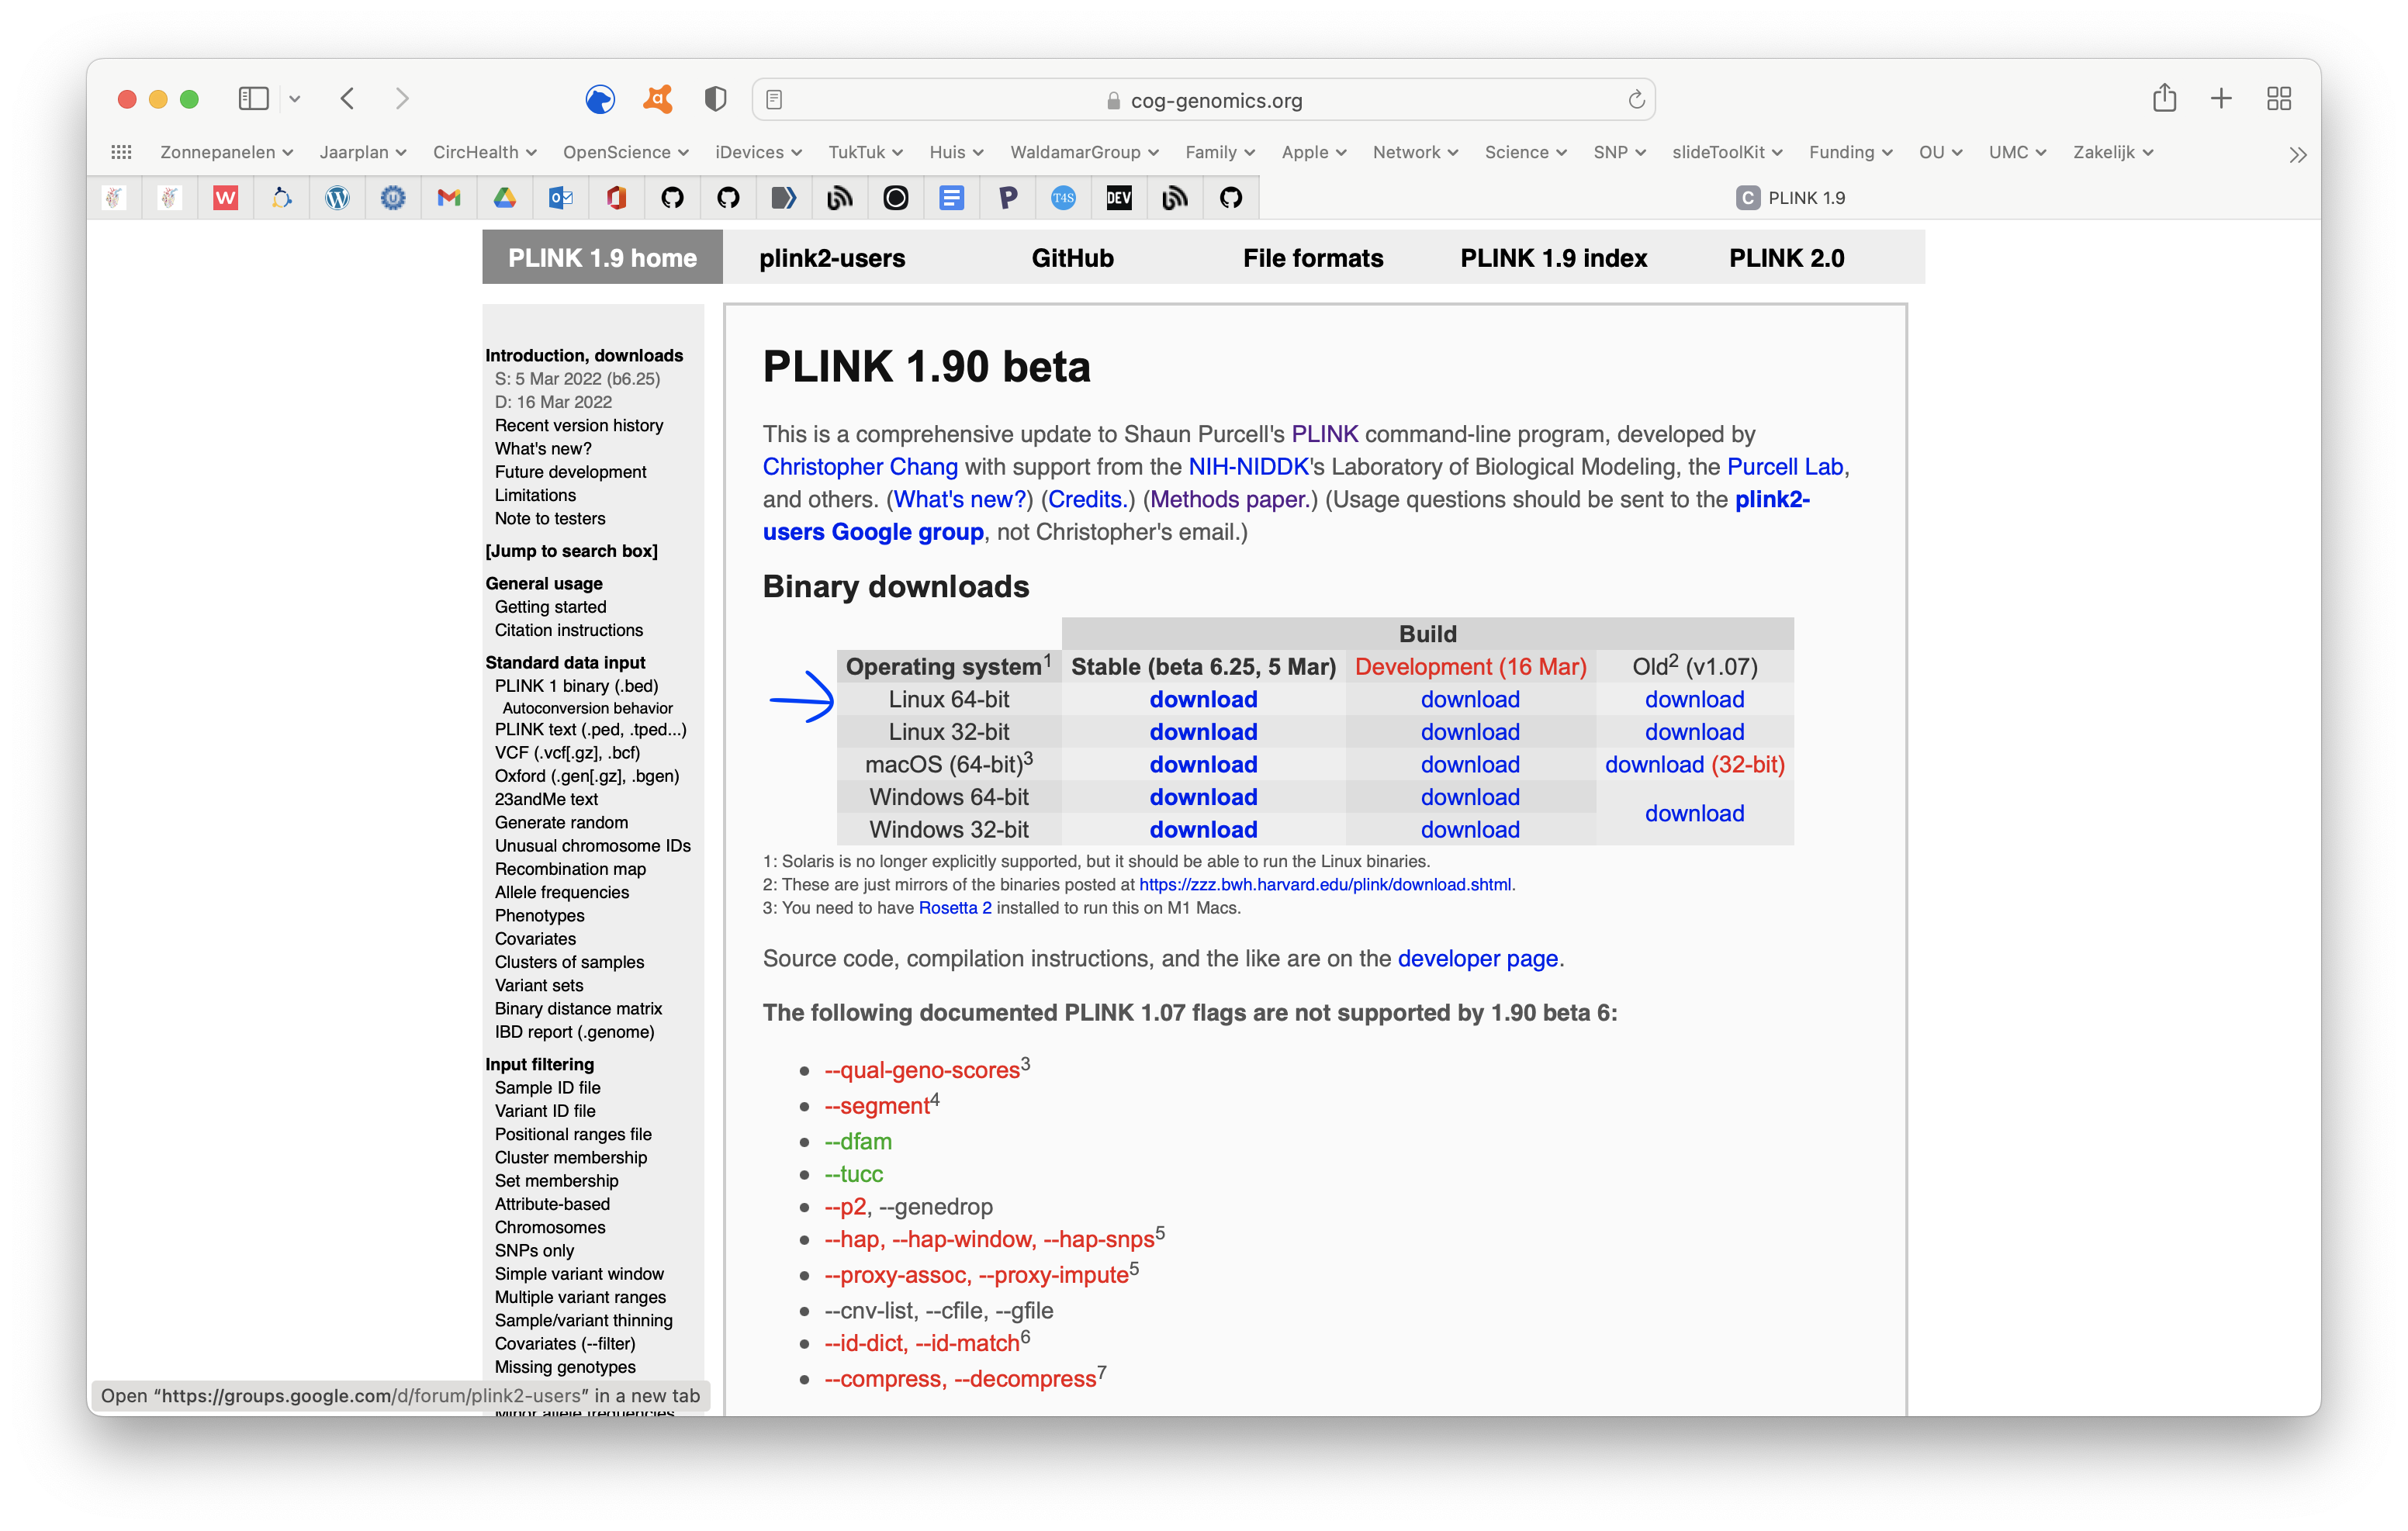
\includegraphics[width=0.85\linewidth]{img/plink} 

}

\caption{The PLINK v1.9 website.}\label{fig:plinkprogram}
\end{figure}

\hypertarget{alternatives-to-plink}{%
\subsection{\texorpdfstring{Alternatives to \texttt{PLINK}}{Alternatives to PLINK}}\label{alternatives-to-plink}}

Nowadays, a lot of people also use programs like \href{snptest}{SNPTEST}, \href{https://data.broadinstitute.org/alkesgroup/BOLT-LMM/}{BOLT-LMM}, \href{http://cnsgenomics.com/software/gcta/\#Overview}{GCTA}, or \href{https://rgcgithub.github.io/regenie/}{regenie} as alternatives to execute GWAS. These programs were designed with specific use-cases in mind, for instance really large biobank data including hundreds of thousands individuals, better control for population stratification, the ability to estimate trait heritability or Fst, and so on.

\hypertarget{other-programs}{%
\subsection{Other programs}\label{other-programs}}

Mendelian randomization can be done either with the \href{http://cnsgenomics.com/software/smr/\#Overview}{SMR} or \href{http://cnsgenomics.com/software/gsmr/}{GSMR} function from GCTA, or with R-packages, like \href{https://mrcieu.github.io/TwoSampleMR/}{\passthrough{\lstinline!TwoSampleMR!}}.

\hypertarget{cocalc}{%
\section{CoCalc}\label{cocalc}}

\begin{quote}
{[} TEXT NEEDS UPDATING{]}
\end{quote}

Now, pay attention. If you came here through the course \textbf{Genetic Epidemiology}, you don't have to do anything. All the data you need are already downloaded.

However, when you are using this book as a standalone, you'll need to start by downloading the data you need for this practical to your Desktop.

For the course we set up a CoCalc Server and everything should be fine; we installed everything you need.

\hypertarget{standalone}{%
\section{Standalone}\label{standalone}}

So, you plan to use this book as `Standalone' on a macOS environment. This means you'll need to install a few things first.

\hypertarget{the-data-you-need}{%
\subsection{The data you need}\label{the-data-you-need}}

You'll need to start by downloading the data you need for this practical to your Desktop.

Here's the link to the data.

\href{https://drive.google.com/drive/folders/1iDLB1y534DfgEZNPCYBrIj5X7g_XlBba?usp=share_link}{Link to Google Drive with data}

Make sure you put the data in the \passthrough{\lstinline!\~/Desktop/practical/!} folder.

The data are pretty large (approx. 15Gb), so this will take a minute or two depending on your internet connection. Time to stretch your legs or grab a coffee (data scientists don't drink tea).

\hypertarget{terminal}{%
\subsection{Terminal}\label{terminal}}

For all the programs we use, except \textbf{RStudio}, you will need the \textbf{Terminal}. This comes with every major operating system; on Windows it is called `PowerShell', but let's not go there. And regardless, you will (have to start to) make your own scripts. The benefit of using scripts is that each step in your workflow is clearly stipulated and annotated, and it allows for greater reproducibility, easier troubleshooting, and scaling up to high-performance computer clusters.

Open the \textbf{Terminal}, it should be on the left in the toolbar as a little black computer-monitor-like icon. Mac users can type \passthrough{\lstinline!command + space!} and type \passthrough{\lstinline!terminal!}, a \textbf{Terminal} screen should open.

\begin{quote}
From now on we will use little code blocks like the example to indicate a code you should type/copy-paste and hit enter. If a code is followed by a comment, it is indicated by a \# - you don't need to copy-paste and execute this.
\end{quote}

\begin{lstlisting}
CODE BLOCK

CODE BLOCK # some comment here
\end{lstlisting}

\hypertarget{navigating-the-terminal}{%
\subsection{Navigating the Terminal}\label{navigating-the-terminal}}

You can navigate around the computer through the terminal by typing \passthrough{\lstinline!cd <path>!}; \passthrough{\lstinline!cd!} stands for ``change directory'' and \passthrough{\lstinline!<path>!} means ``some\_file\_directory\_you\_want\_to\_go\_to''.

This command will bring you to your home directory.

\begin{lstlisting}
cd ~ 
\end{lstlisting}

This will bring you to the parent directory (up one level).

\begin{lstlisting}
cd ../ 
\end{lstlisting}

This will bring you to the XXX directory.

\begin{lstlisting}
cd XXX 
\end{lstlisting}

Let's navigate to the folder you just downloaded.

\begin{lstlisting}
cd ~/Desktop/practical
\end{lstlisting}

Let's check out what is inside the directory, by listing (\passthrough{\lstinline!ls!}) its contents.

This command shows files as list; the \passthrough{\lstinline!-l!} makes it a vertical list and adds more information, you can also remove it and simply type \passthrough{\lstinline!ls!} - go on, and try.

\begin{lstlisting}
ls -l 
\end{lstlisting}

This command shows files as list with human readable format.

\begin{lstlisting}
ls -lh 
\end{lstlisting}

Adding the flags \passthrough{\lstinline!-lh!} will get you the contents of a directory in a list (\passthrough{\lstinline!-l!}) and make the size `human-readable' (\passthrough{\lstinline!-h!}).

Adding \passthrough{\lstinline!-t!} shows the files as list sorted by time edited.

\begin{lstlisting}
ls -lt 
\end{lstlisting}

Adding \passthrough{\lstinline!-S!} shows the files as list sorted by size.

\begin{lstlisting}
ls -lS 
\end{lstlisting}

You can also count the number of files. Just `pipe' the result from \passthrough{\lstinline!ls!} to the next program \passthrough{\lstinline!wc!} (`wordcount') and list the number of lines, \passthrough{\lstinline!-l!}. In this case \passthrough{\lstinline!-l!} is a flag used by \passthrough{\lstinline!wc!} and it has a different meaning than it does for \passthrough{\lstinline!ls!}.

\begin{lstlisting}
ls | wc -l
\end{lstlisting}

And if you want to know all the function of a program simply type the following.

\begin{lstlisting}
man ls
\end{lstlisting}

This will take you to a manual of the program with an extensive description of each flag (Figure \ref{fig:lsmanual}).

\begin{figure}[H]

{\centering 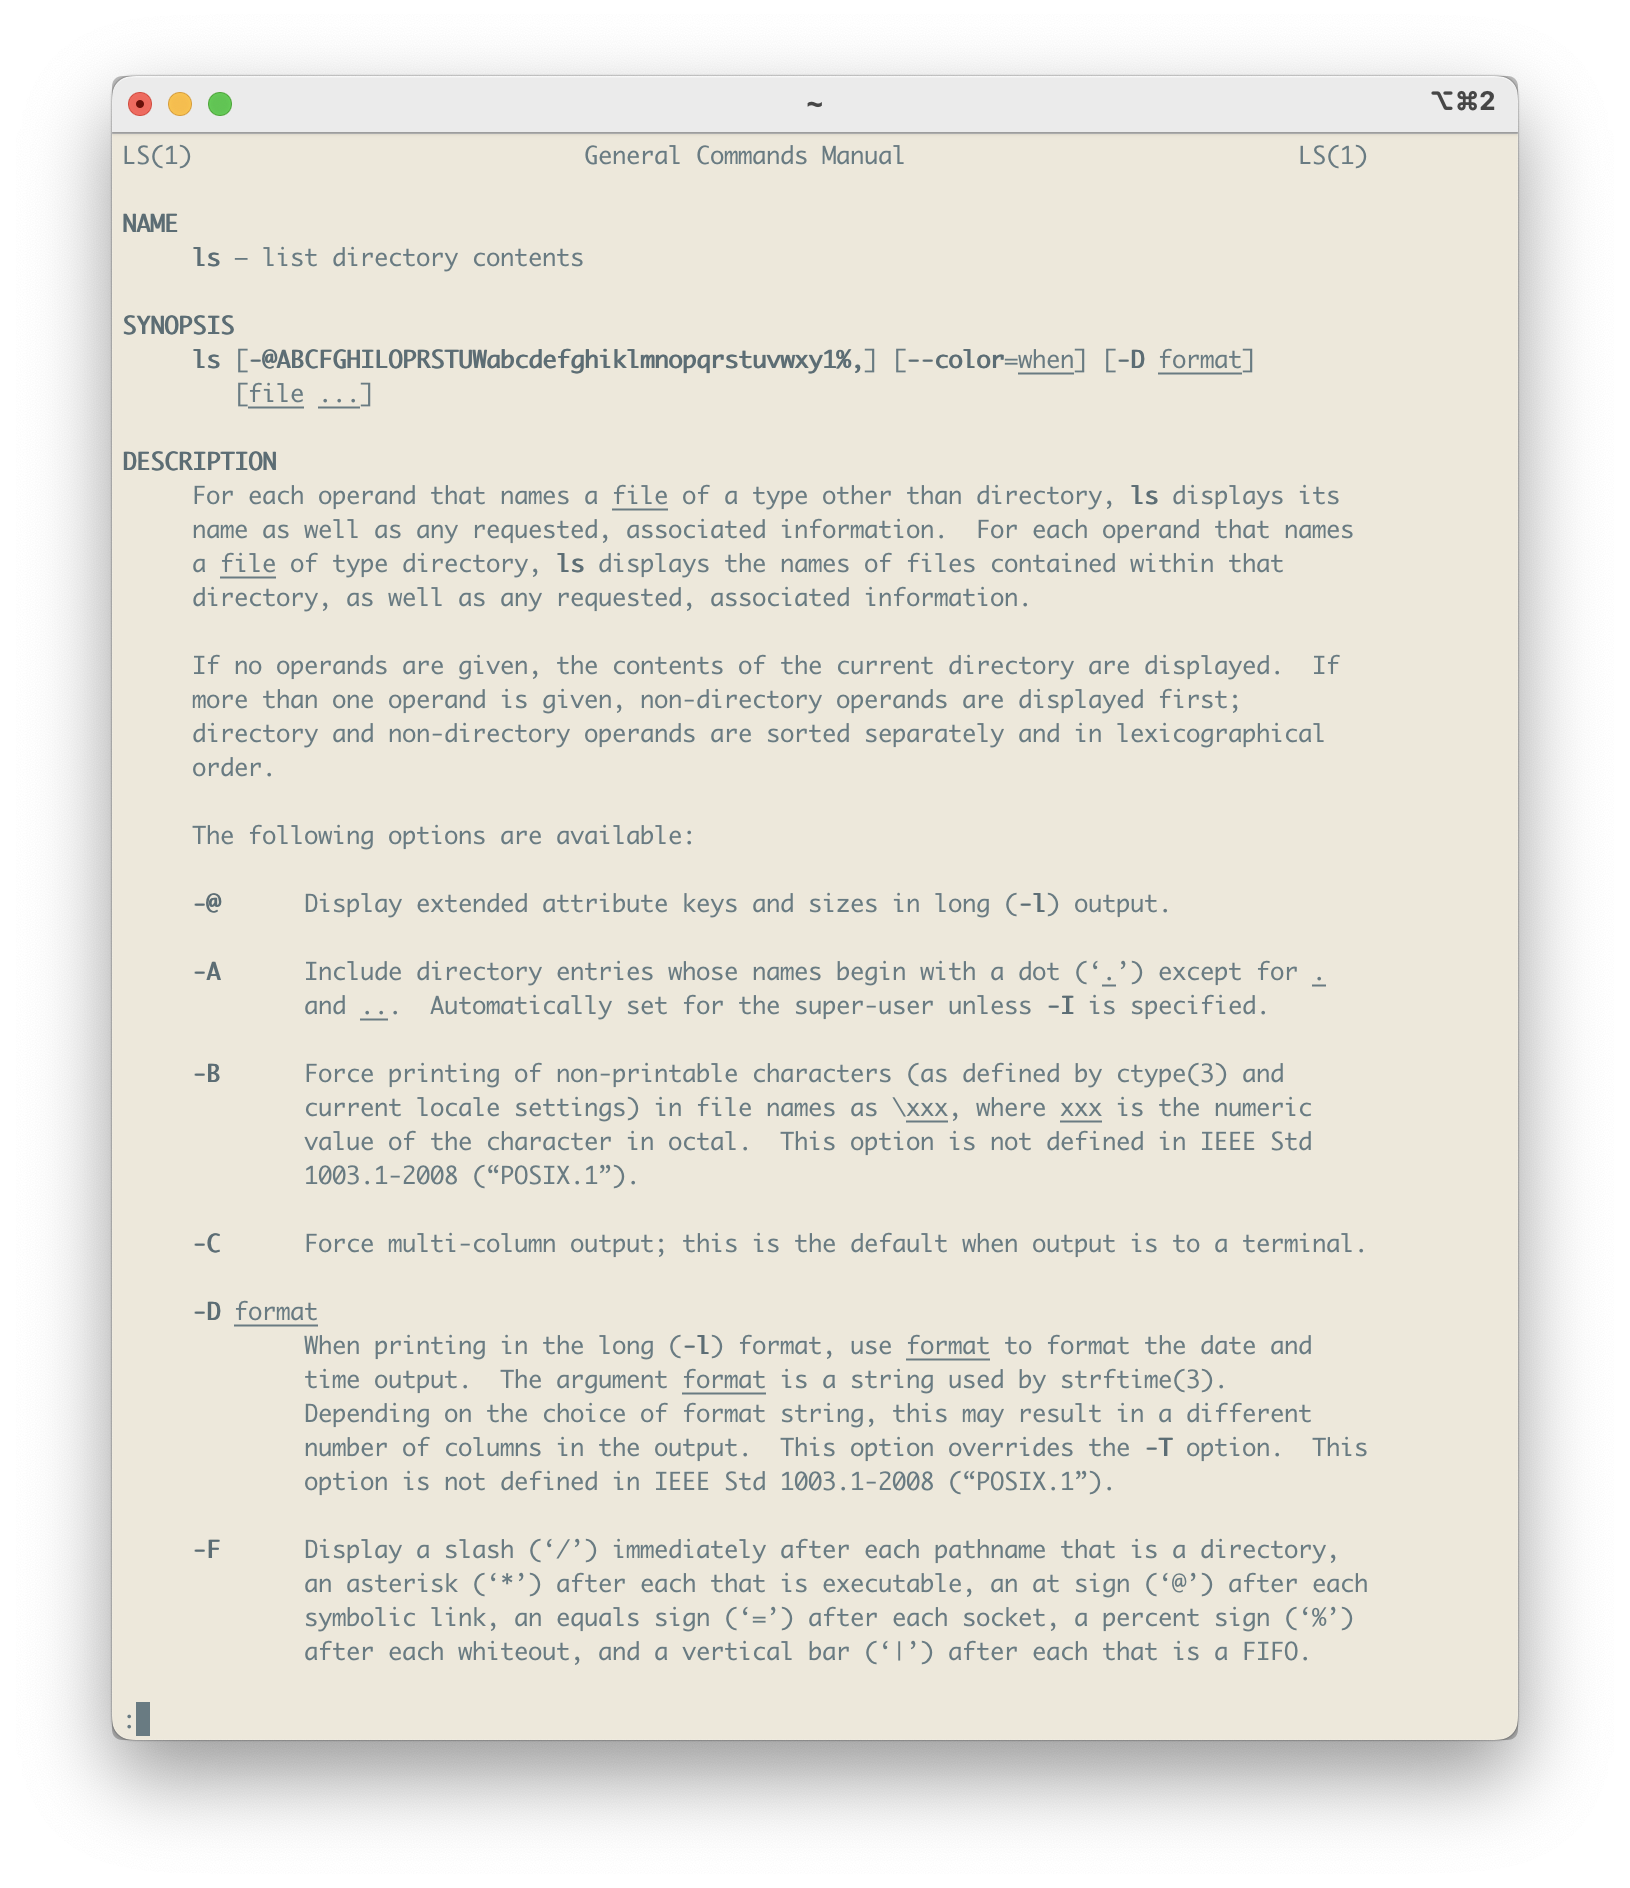
\includegraphics[width=0.85\linewidth]{img/ls_manual} 

}

\caption{Partial output from the ls manual.}\label{fig:lsmanual}
\end{figure}

\hypertarget{installing-the-software}{%
\subsection{Installing the software}\label{installing-the-software}}

\hypertarget{brew}{%
\subsubsection{brew}\label{brew}}

Linux has a great package-manager that is lacking on macOS. You can install \href{https://brew.sh}{\passthrough{\lstinline!brew!}} to compensate for this. This adds the ability to install almost any Linux-based program through the \textbf{Terminal} such as \passthrough{\lstinline!wget!}, \passthrough{\lstinline!llvm!}, etc.

Open \textbf{Terminal} and execute the following:

\begin{lstlisting}
/bin/bash -c "$(curl -fsSL https://raw.githubusercontent.com/Homebrew/install/HEAD/install.sh)"
\end{lstlisting}

Check if everything is in order.

\begin{lstlisting}
brew doctor
\end{lstlisting}

It shouldn't report any errors.

\hypertarget{plink-1}{%
\subsubsection{PLINK}\label{plink-1}}

First, we'll get \passthrough{\lstinline!PLINK!}. Navigate to the \textbf{PLINK v1.9} website, which can be found \href{https://www.cog-genomics.org/plink2}{here}. Download the macOS (64-bit) version under `Stable (beta x.x, day month year)'.

\begin{quote}
Note: Apple produced Intel-based computers for a few years back, and most programs, packages, libraries and whatnot are designed for that. So, I highly recommend using software designed for that and activating Rosetta2 in your Terminal. Don't know how to do that? Following \href{https://support.apple.com/en-us/102527}{these instructions}.
\end{quote}

Unzip the folder and put \passthrough{\lstinline!plink!} in the practical folder.

\begin{lstlisting}
mv -v ~/Downloads/plink_mac_20231211/plink ~/Desktop/practical/plink 
\end{lstlisting}

\hypertarget{installing-r-and-rstudio}{%
\subsubsection{Installing R and RStudio}\label{installing-r-and-rstudio}}

Let's go ahead and use \passthrough{\lstinline!brew!} to install the \passthrough{\lstinline!R!} and \textbf{RStudio} software.

In \textbf{Terminal} execute the following and just follow the instructions.

\begin{lstlisting}
brew install rstudio
brew install --cask r
\end{lstlisting}

Now close the terminal window - really make sure that the terminal-program has quit.

Open your fresh installation of \textbf{RStudio} by double clicking the icon. You should be seeing something like figure \ref{fig:rstudioscreenshot}

\begin{figure}[H]

{\centering 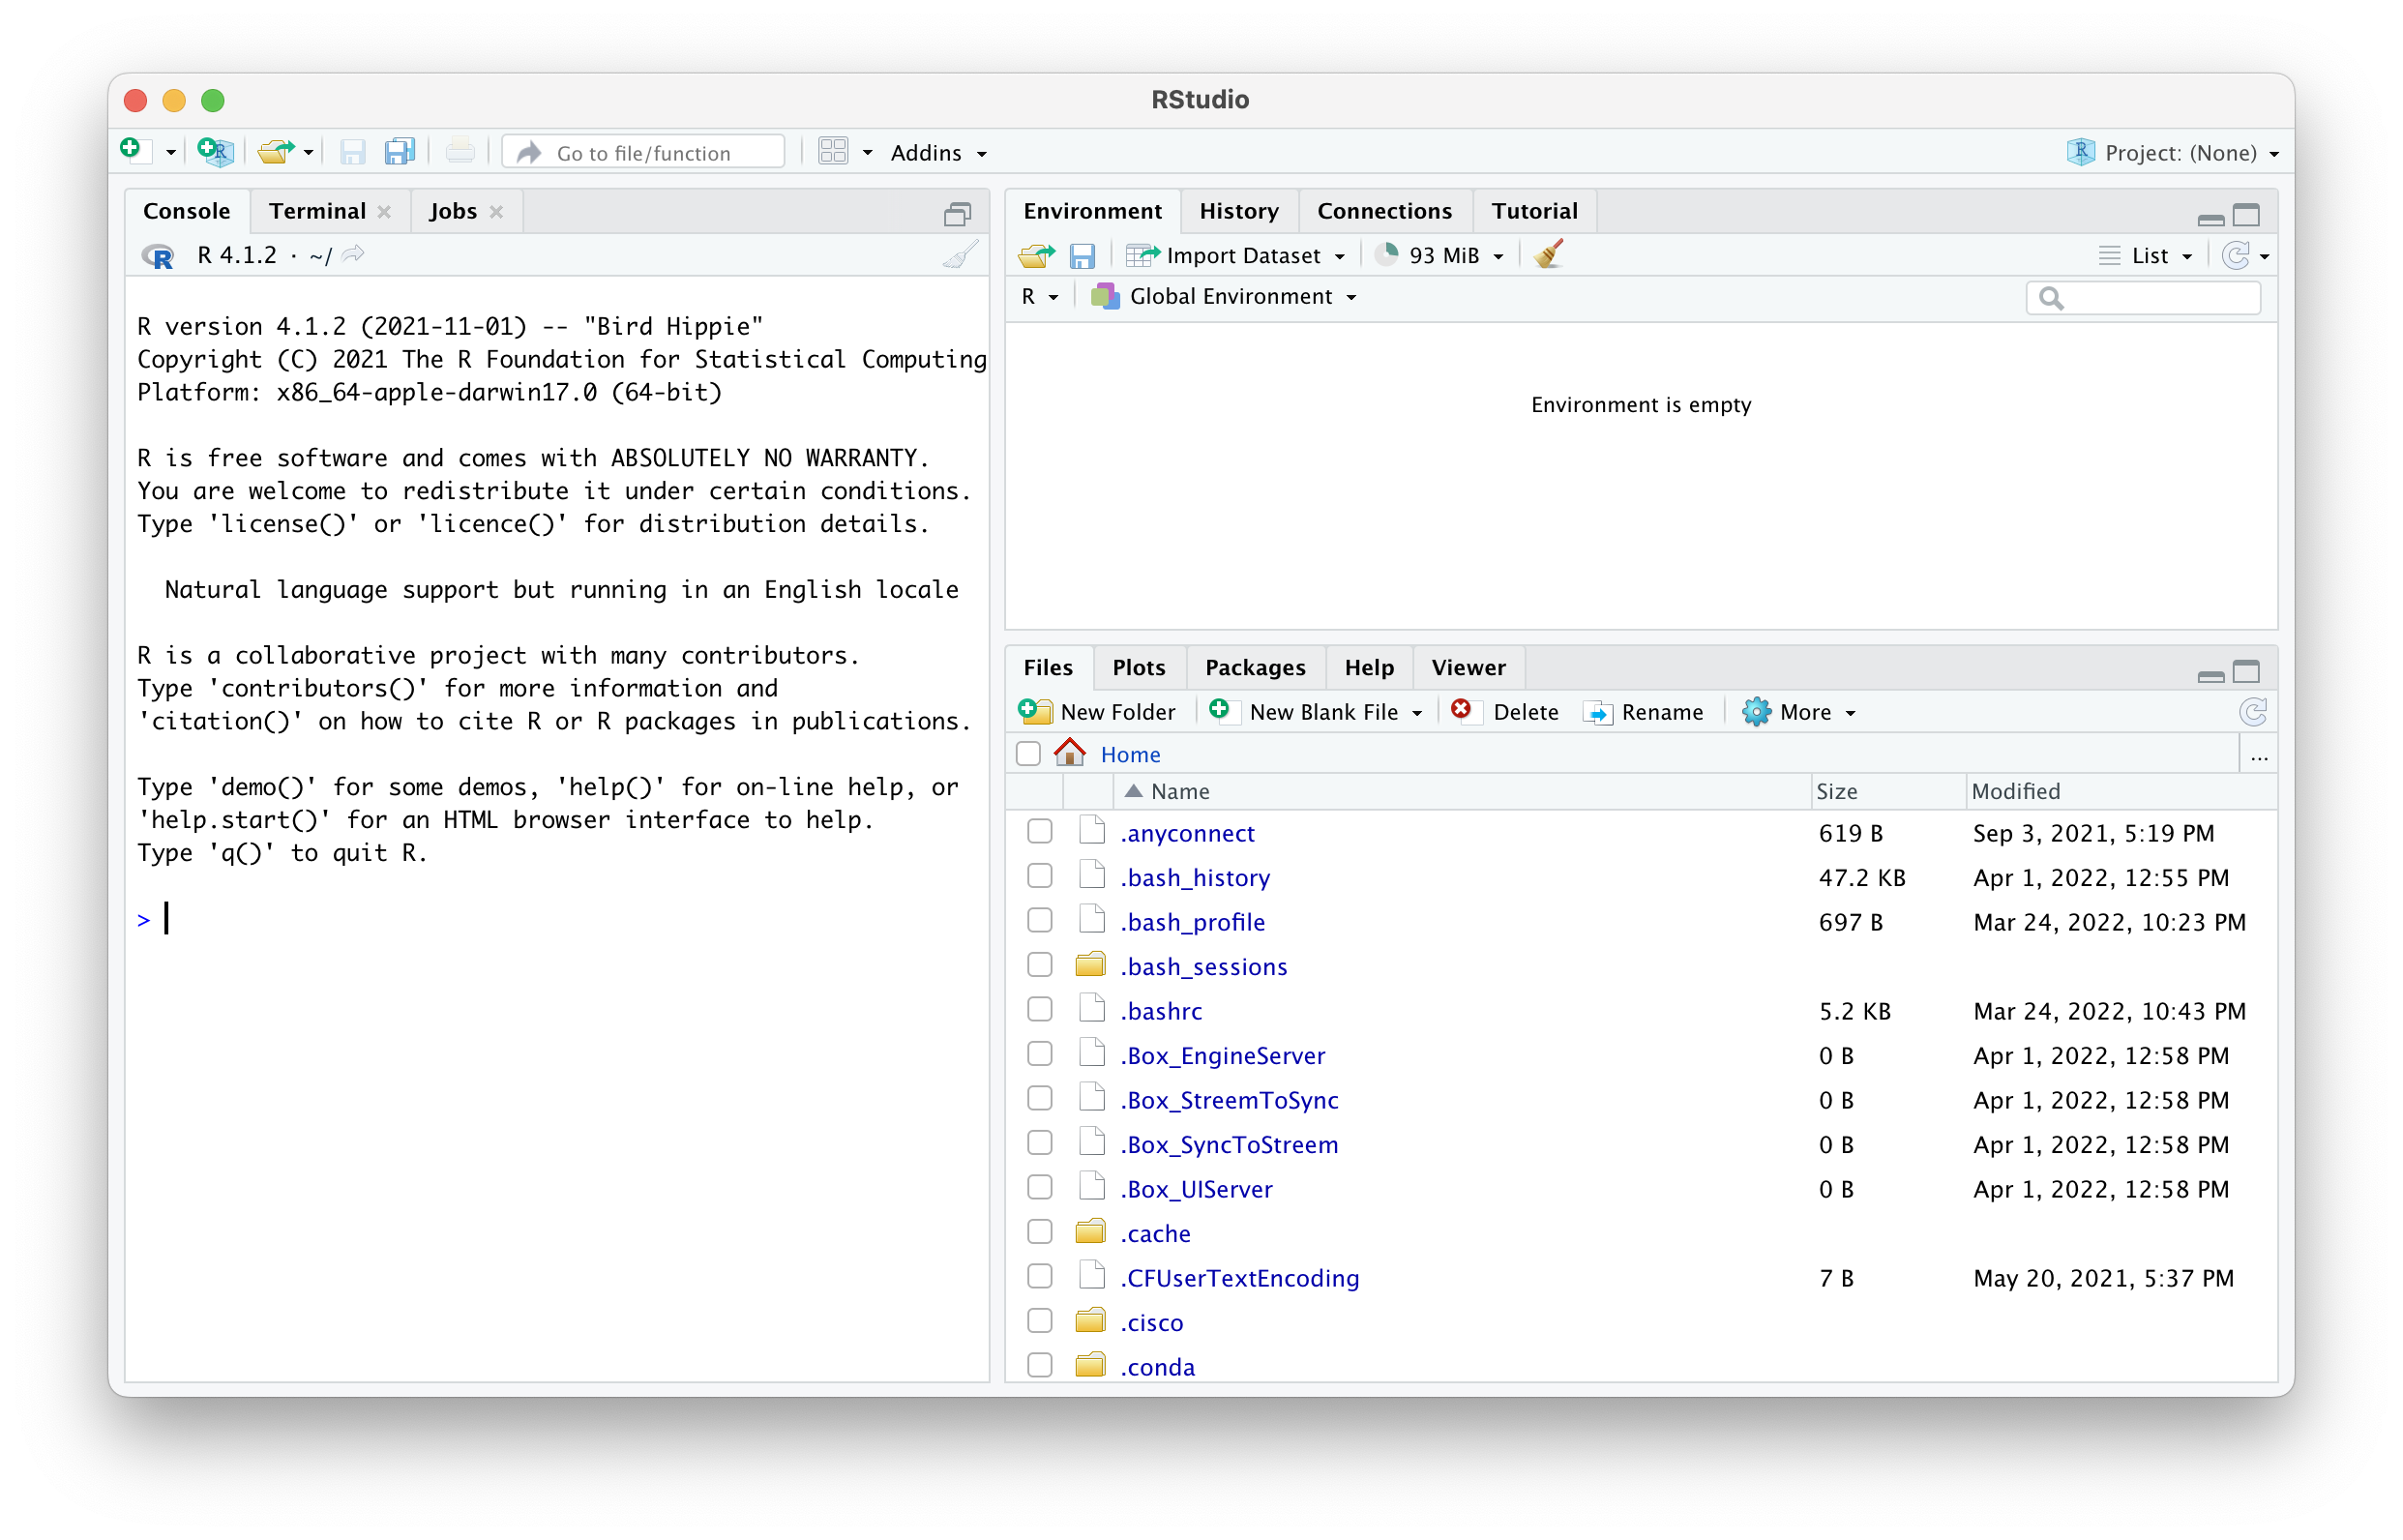
\includegraphics[width=0.85\linewidth]{img/rstudio-screenshot} 

}

\caption{RStudio screenshot.}\label{fig:rstudioscreenshot}
\end{figure}

In the top right, you see a little green-white plus-sign, click this and select `R Notebook' (Figure \ref{fig:rstudioscreenshotcreatenotebook}).

\begin{figure}[H]

{\centering 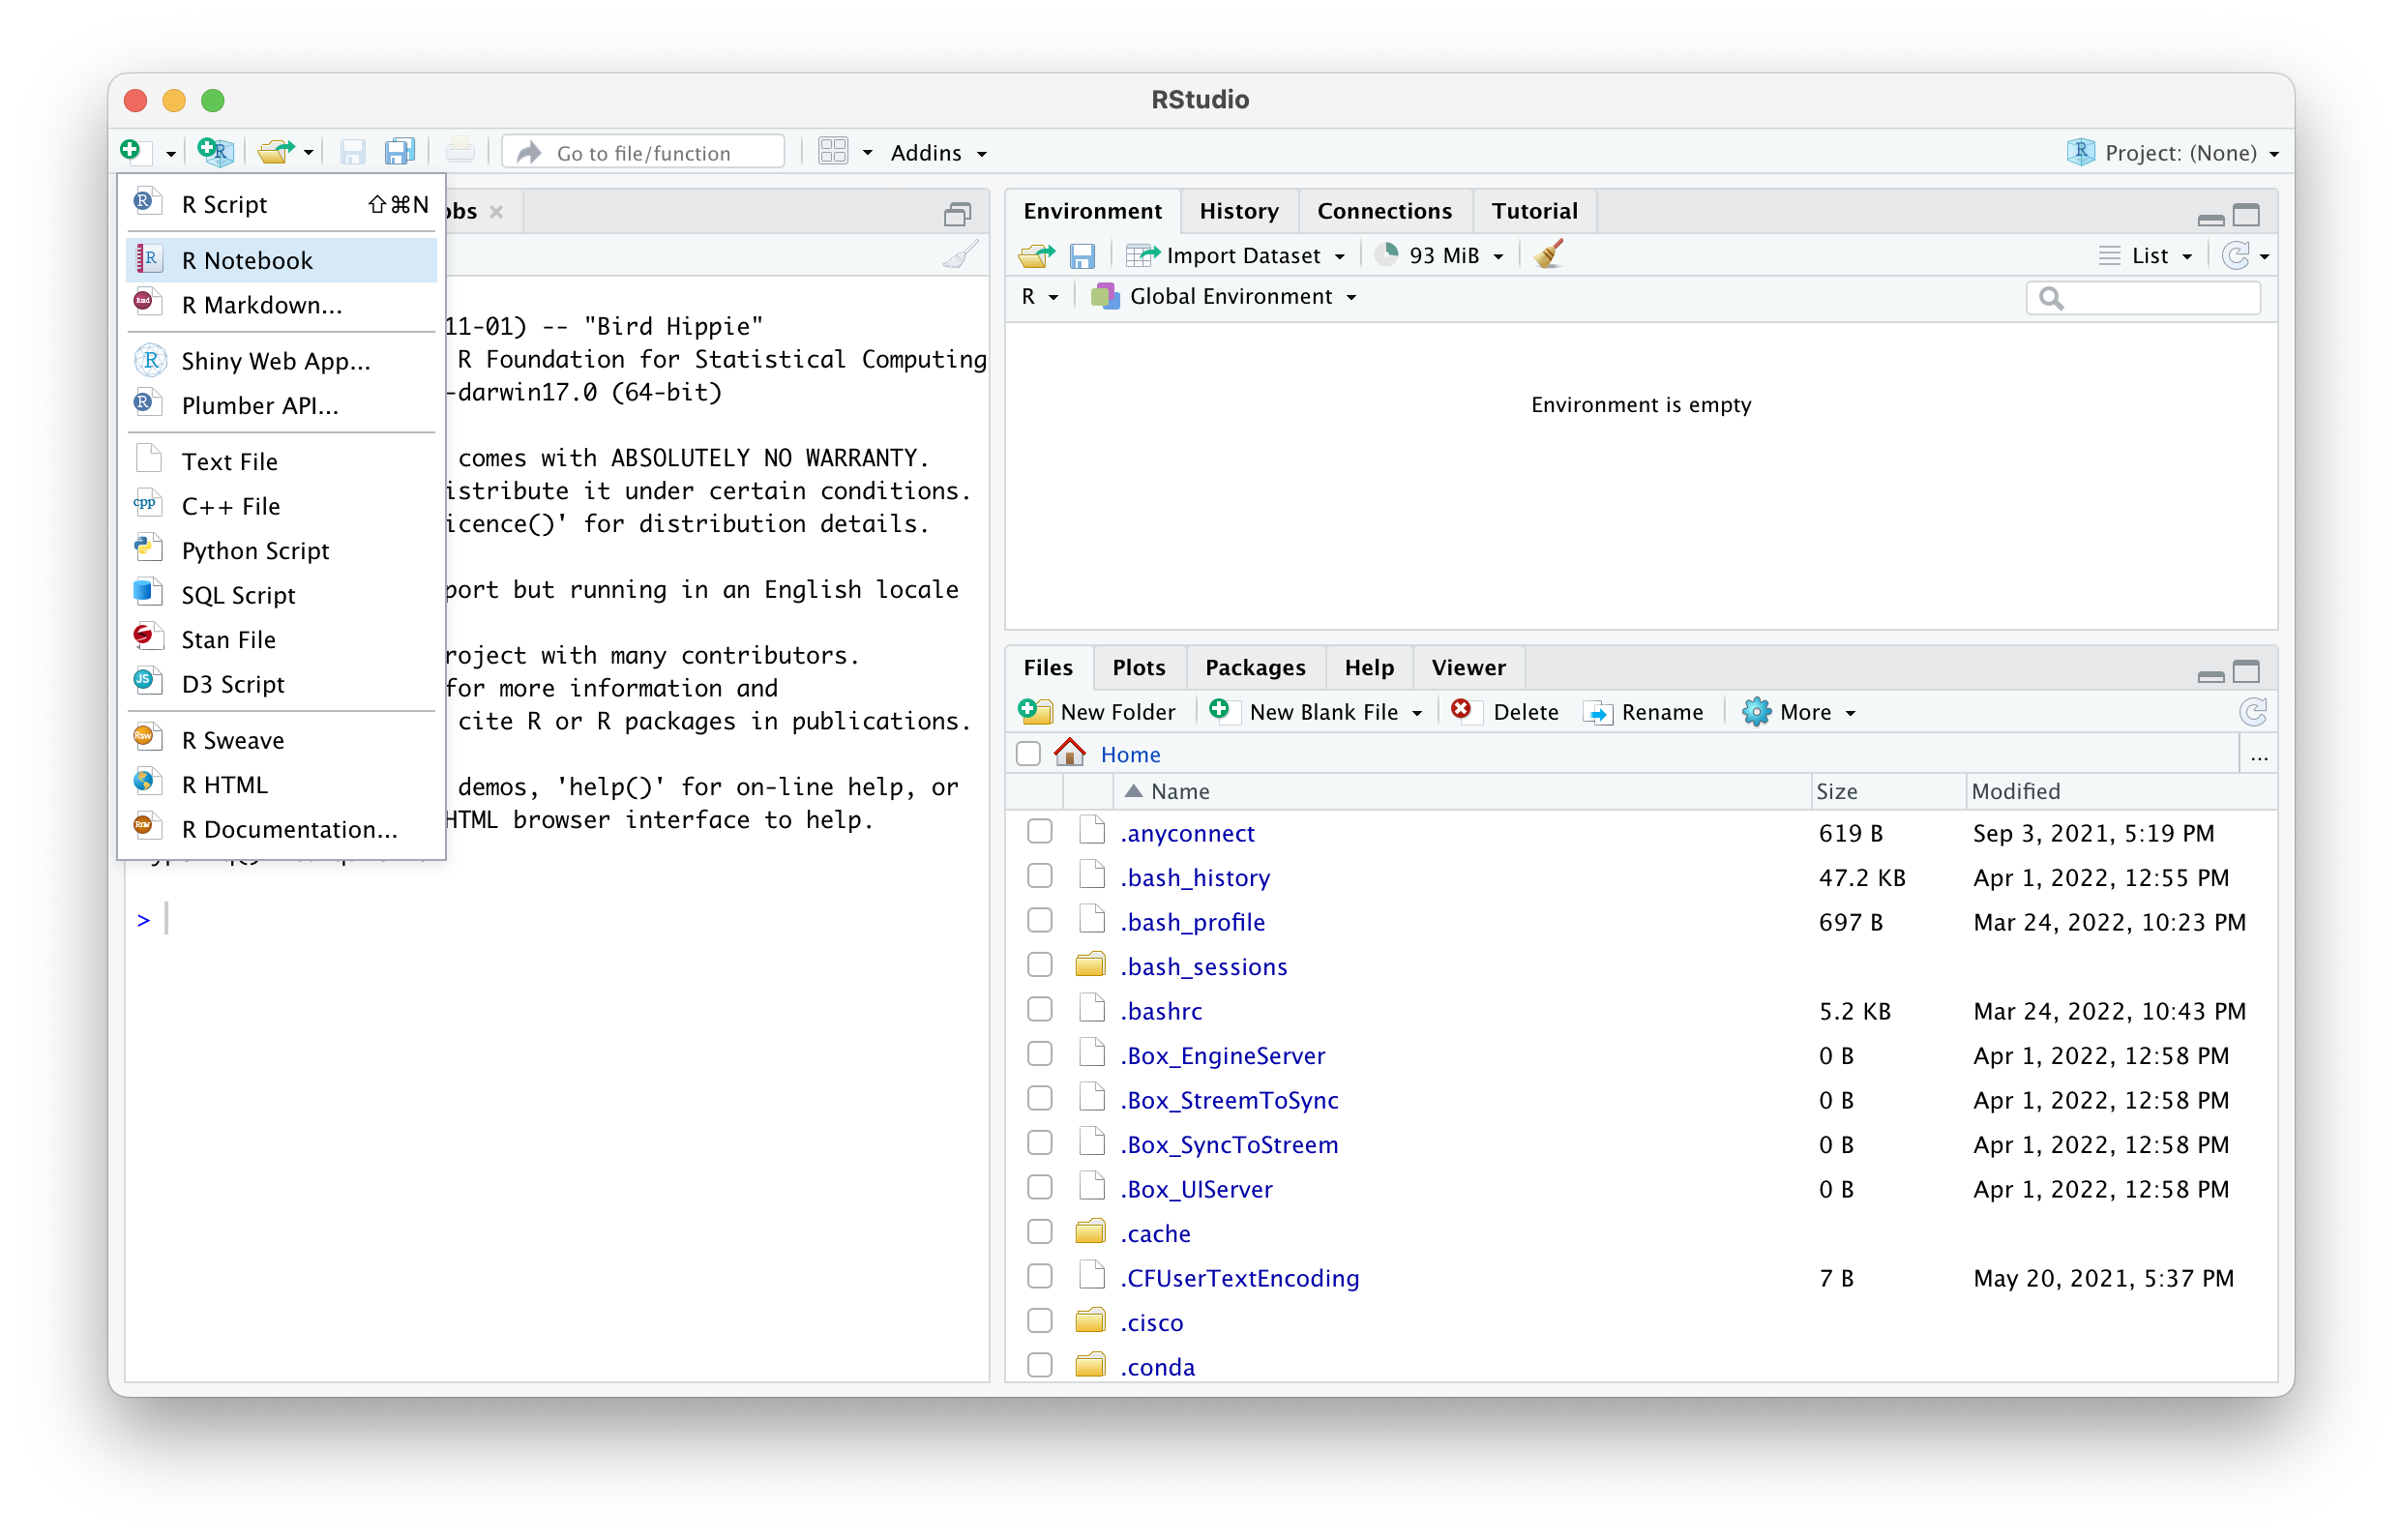
\includegraphics[width=0.85\linewidth]{img/rstudio-screenshot-create-notebook} 

}

\caption{RStudio screenshot.}\label{fig:rstudioscreenshotcreatenotebook}
\end{figure}

You will create an untitled (\passthrough{\lstinline!Untitled1!}) \passthrough{\lstinline!R!} notebook: you can combine text descriptions, like you would in a lab-journal, with code-sections. Read what is in the notebook to get a grasp on that (Figure \ref{fig:rstudioscreenshotnotebook}).

\begin{figure}[H]

{\centering 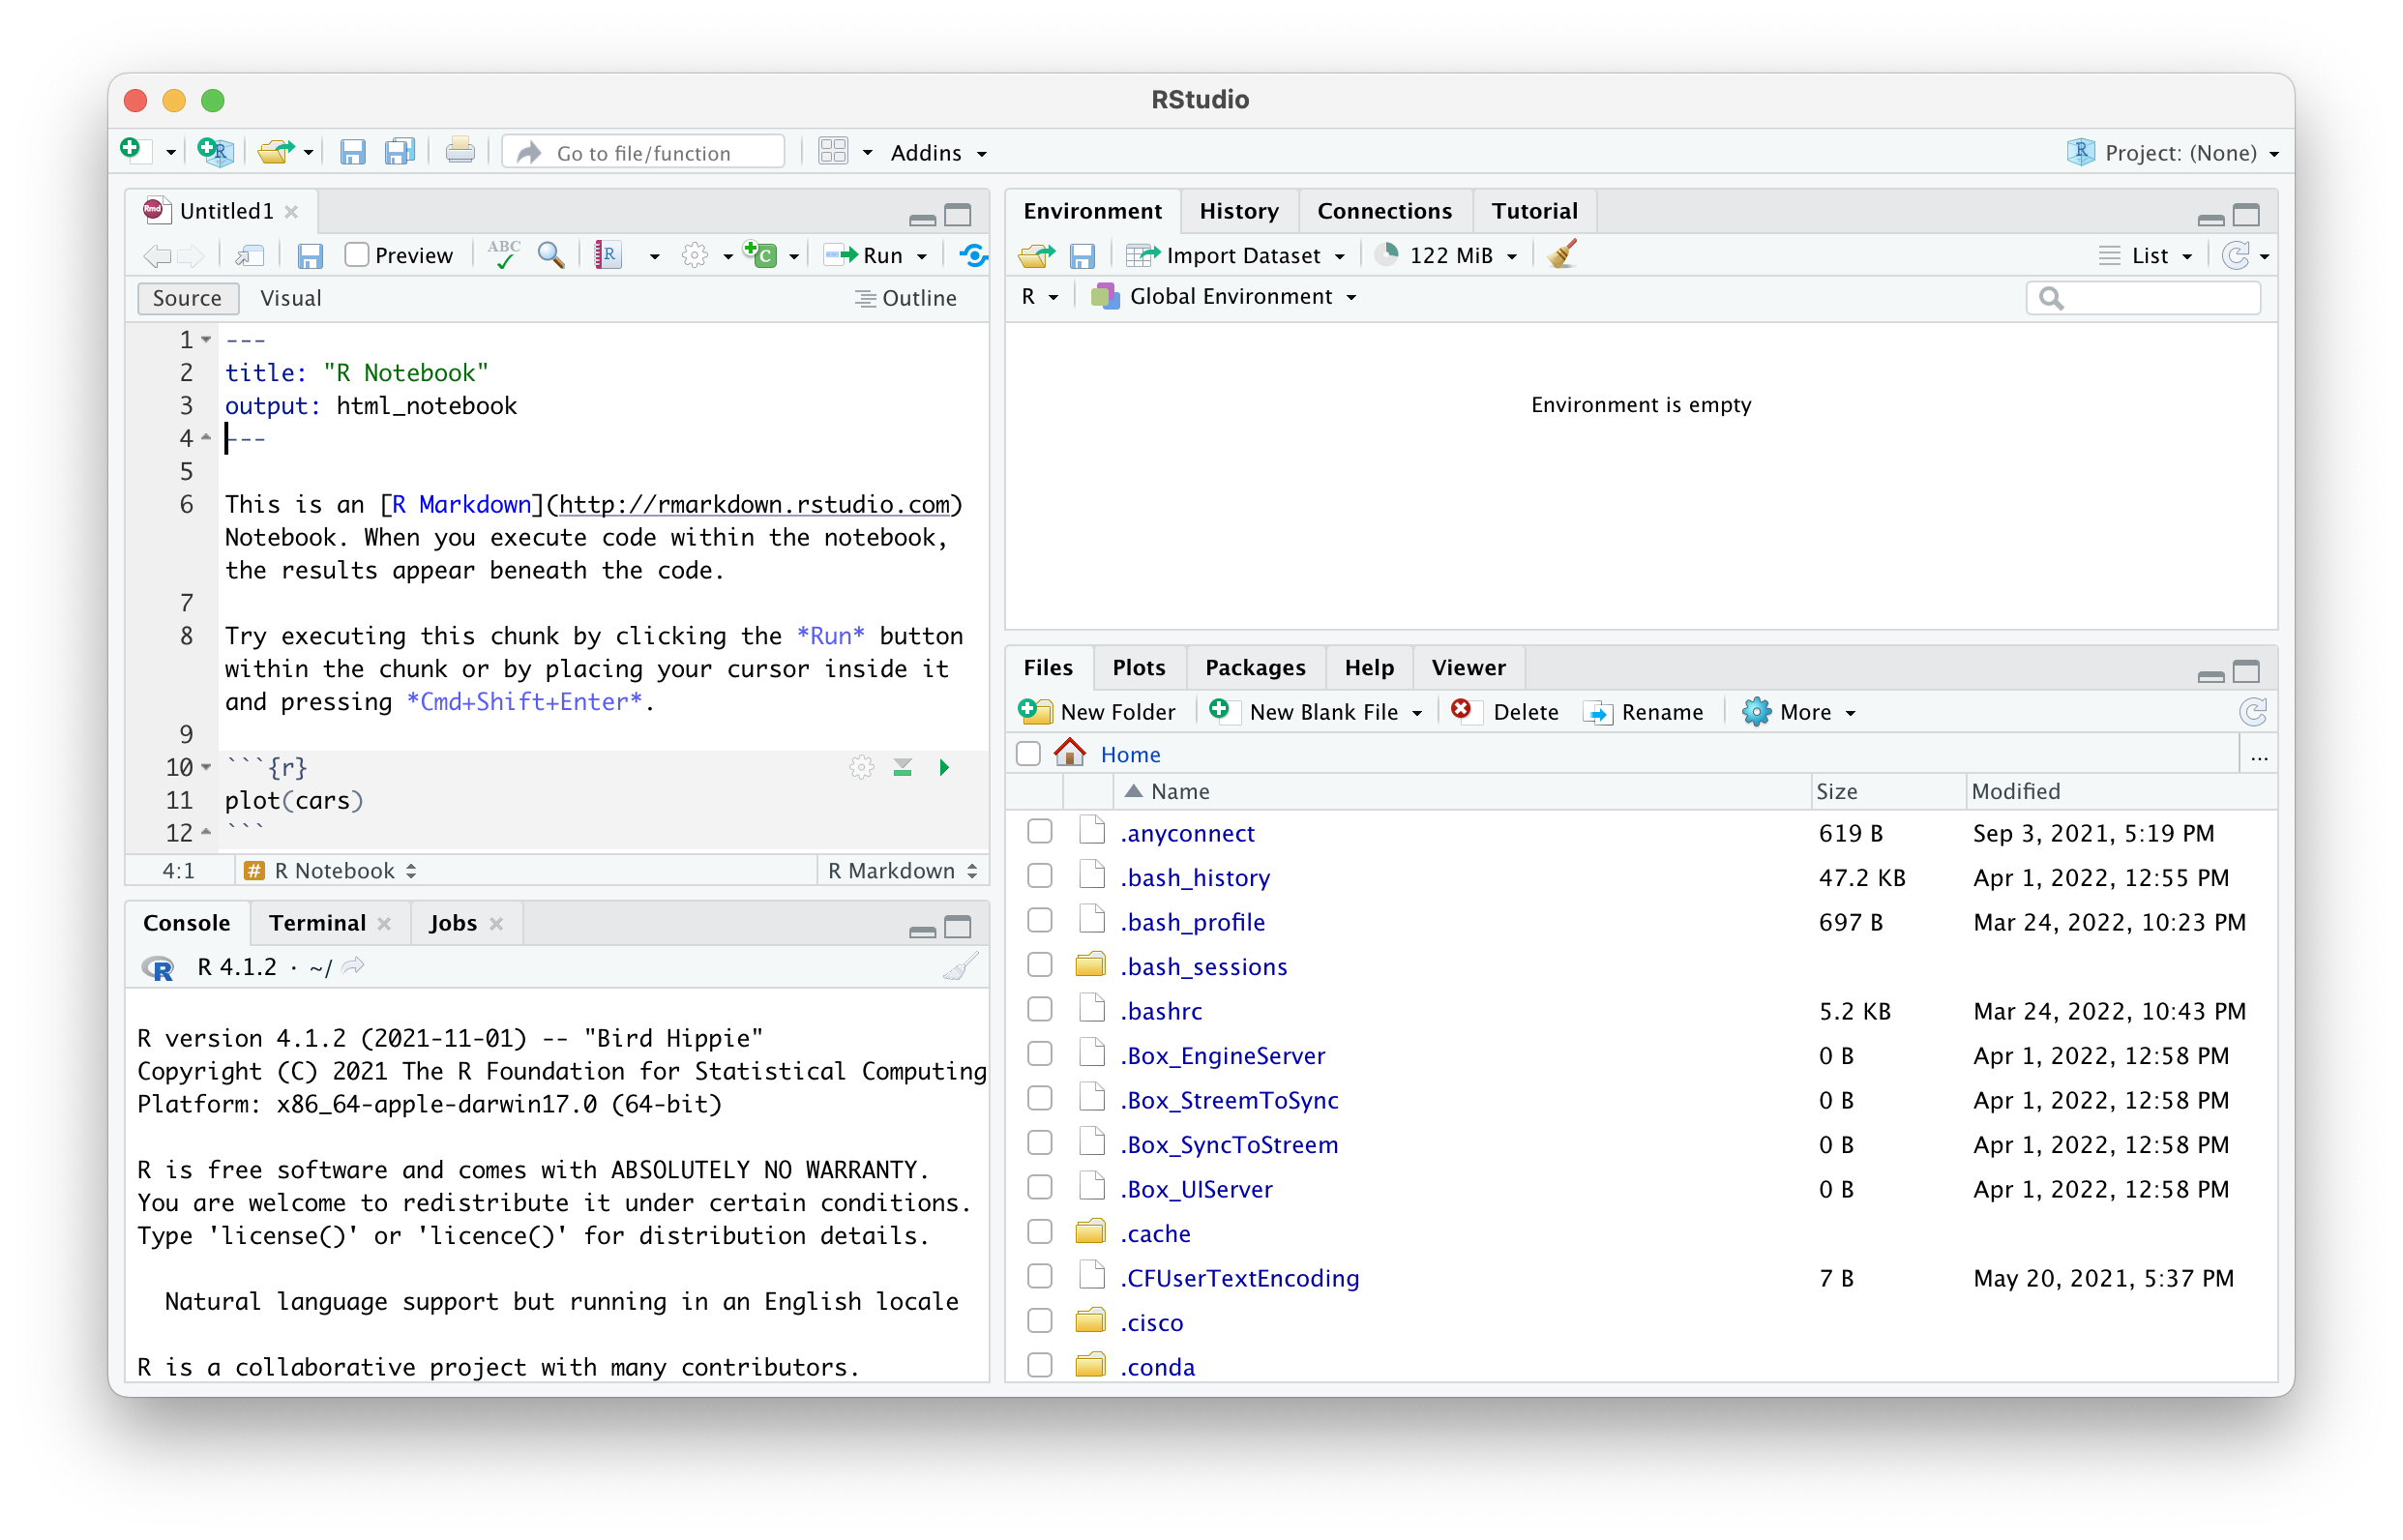
\includegraphics[width=0.85\linewidth]{img/rstudio-screenshot-notebook} 

}

\caption{RStudio screenshot.}\label{fig:rstudioscreenshotnotebook}
\end{figure}

Right, you should be installing some packages. To do so, you can remove \passthrough{\lstinline!plot(cars)!} (or leave and create a new code-block as per instructions in the notebook), and copy paste the code below. Make sure to put in a code block like the example in which \passthrough{\lstinline!plot(cars)!} is in.

\begin{lstlisting}
remotes::install_github(c("rstudio/rmarkdown"))

install.packages(c("formatR", "remotes", 
                   "httr", "usethis", 
                   "data.table", "devtools", 
                   "dplyr", "tibble", "tidyverse", 
                   "openxlsx",
                   "ggplot2",
                   "ggsci", "ggthemes",
                   "qqman", "CMplot", "plotly", 
                   "openxlsx"))
devtools::install_github("kassambara/ggpubr")

devtools::install_github("oliviasabik/RACER")

remotes::install_github("MRCIEU/TwoSampleMR")
devtools::install_github("MRCIEU/MRInstruments")

if (!require("BiocManager", quietly = TRUE))
  install.packages("BiocManager")
BiocManager::install("geneplotter")
\end{lstlisting}

You should load these packages too.

\begin{lstlisting}
library(rmarkdown)
library(formatR)

library(openxlsx)

library(data.table)

library(tibble)
library(tidyverse)
library(dplyr)
library(plotly)

library(ggplot2)
library(devtools)
library(ggpubr)
library(ggsci)
library(ggthemes)

library(qqman)
library(CMplot)
library(RACER)

library(remotes)
library(TwoSampleMR)
library(MRInstruments)

library("geneplotter")
\end{lstlisting}

All in all this may take some time, good moment to relax, review your notes, stretch your legs, or take a coffee.

\hypertarget{are-you-ready}{%
\section{Are you ready?}\label{are-you-ready}}

Are you ready? Did you bring coffee and a good dose of energy? Let's start!

Oh, one more thing: you can save your notebook, the one you just created, to keep all the \passthrough{\lstinline!R!} codes you are applying in the next chapters and add descriptions and notes. If you save this notebook you'll notice that a \passthrough{\lstinline!html!}-file is created. This file is a legible webbrowser-friendly version of your work and contains the codes and the output (code messages, tables, and figures). And the nice thing is, that you can easily share it with others over email.

Ok. 'Nough said, let's move on to cover some basics in Chapter \ref{gwas-basics}.

\hypertarget{gwas-basics}{%
\chapter{Steps in a Genome-Wide Association Study}\label{gwas-basics}}

Now that you understand a bit of the navigation in Unix-systems, you're ready to start this practical primer. We will make use of a dummy dataset containing cases and controls. We will explain and execute the following steps:

\begin{enumerate}
\def\labelenumi{\arabic{enumi}.}
\tightlist
\item
  convert raw data to a more memory-efficient format
\item
  apply extensive quality control on samples and SNPs
\item
  assess the ancestral background of your study population
\item
  perform association testing
\item
  visualize association results
\end{enumerate}

\hypertarget{converting-datasets}{%
\section{Converting datasets}\label{converting-datasets}}

The format in which genotype data are returned to investigators varies among genome-wide SNP platforms and genotyping centers. Usually genotypes have been called by a genotyping center and returned in the standard \passthrough{\lstinline!PED!} and \passthrough{\lstinline!MAP!} file formats designed for \passthrough{\lstinline!PLINK!}.

A \passthrough{\lstinline!PED!} file is a white space (space or tab)-delimited file in which each line represents one individual and the first six columns are mandatory and in the following order:

\begin{itemize}
\tightlist
\item
  `Family ID',
\item
  `Individual ID',
\item
  `Paternal ID',
\item
  `Maternal ID',
\item
  `Sex (1=male, 2=female, 0=missing)', and
\item
  `Phenotype (1=unaffected, 2=affected, 0=missing)'.
\end{itemize}

The subsequent columns denote genotypes that can be any character (e.g., 1, 2, 3, 4 or A, C, G, T). Zero denotes a missing genotype. Each SNP must have two alleles (i.e., both alleles are either present or absent).
The order of SNPs in the PED file is given in the MAP file, in which each line denotes a single marker and the four white-space--separated columns are chromosome (1--22, X, Y or 0 for unplaced), marker name (typically an rs number), genetic distance in Morgans (this can be fixed to 0) and base-pair position (bp units).

Let's start by using \passthrough{\lstinline!PLINK!} to converting the datasets to a lighter, binary form (a \passthrough{\lstinline!.bed!}-file). This file saves data in a more memory- and time-efficient manner (in a `binary'-format) to facilitate the analysis of large-scale data sets \citep{purcell2007}. The marker-information is stored in the \passthrough{\lstinline!.bim!}-file and the family information in the \passthrough{\lstinline!.fam!}-file. \passthrough{\lstinline!PLINK!} creates a \passthrough{\lstinline!.log!} file (named \passthrough{\lstinline!raw-GWA-data.log!}) that details (among other information) the implemented commands, the number of cases and controls in the input files, any excluded data and the genotyping rate in the remaining data. This file is very useful for checking whether the software is successfully completing commands.

Make sure you are in the right directory. Do you remember how to get there?

\begin{lstlisting}
cd ~/Desktop/practical
\end{lstlisting}

Next, we'll make a project directory.

\begin{lstlisting}
mkdir -v ~/Desktop/practical/dummy_project
\end{lstlisting}

Now, we'll convert the \passthrough{\lstinline!.ped!}/\passthrough{\lstinline!.map!} files to the binary-format.

\begin{lstlisting}
plink --file rawdata/raw-GWA-data --make-bed --out dummy_project/rawdata
\end{lstlisting}

Let's review the \passthrough{\lstinline!.log!}-file for a bit. It should look something like this:

\begin{lstlisting}
PLINK v1.90b7.2 64-bit (11 Dec 2023)           www.cog-genomics.org/plink/1.9/
(C) 2005-2023 Shaun Purcell, Christopher Chang   GNU General Public License v3
Logging to dummy_project/rawdata.log.
Options in effect:
  --file rawdata/raw-GWA-data
  --make-bed
  --out dummy_project/rawdata

16384 MB RAM detected; reserving 8192 MB for main workspace.
.ped scan complete (for binary autoconversion).
Performing single-pass .bed write (317503 variants, 2000 people).
--file: dummy_project/rawdata-temporary.bed +
dummy_project/rawdata-temporary.bim + dummy_project/rawdata-temporary.fam
written.
317503 variants loaded from .bim file.
2000 people (997 males, 1003 females) loaded from .fam.
2000 phenotype values loaded from .fam.
Using 1 thread (no multithreaded calculations invoked).
Before main variant filters, 2000 founders and 0 nonfounders present.
Calculating allele frequencies... done.
Warning: 11440 het. haploid genotypes present (see dummy_project/rawdata.hh );
many commands treat these as missing.
Total genotyping rate is 0.985682.
317503 variants and 2000 people pass filters and QC.
Among remaining phenotypes, 1023 are cases and 977 are controls.
--make-bed to dummy_project/rawdata.bed + dummy_project/rawdata.bim +
dummy_project/rawdata.fam ... done.
\end{lstlisting}

So, there are 317,503 variants included for 2,000 people, 997 males and 1,003 females. All of these individuals are \href{https://www.cog-genomics.org/plink/1.9/filter\#nonfounders}{`founders'}. There are 1,023 cases and 977 controls. The genotyping rate is about 98.6\% which is pretty good. Lastly, there are 11,440 heterozygous haploid genotypes present.

\begin{quote}
Question: Can you think off what the `11,440 heterozygous haploid genotypes present' represent?
\end{quote}

\hypertarget{quality-control}{%
\section{Quality control}\label{quality-control}}

We are ready for some quality control and quality assurance, heavily inspired by Anderson \emph{et al.} \citep{anderson2010} and Laurie \emph{et al.} \citep{laurie2010}. In general, we should check out a couple of things regarding the data quality on two levels:

\begin{enumerate}
\def\labelenumi{\arabic{enumi})}
\tightlist
\item
  samples
\item
  variants
\end{enumerate}

So, we will investigate the following:

\begin{itemize}
\tightlist
\item
  Are the \emph{sexes} based on genetic data matching the ones given by the phenotype file?
\item
  Identify individuals that are outliers in terms of missing data (\emph{call rate}) or heterozygosity rates. This could indicate a genotyping error or sample swap.
\item
  Identify duplicated or related individuals.
\item
  Identify individuals with divergent ancestry.
\item
  What are the allele frequencies?
\item
  What is the per-SNP call rate?
\item
  In the case of a case-control study (which is the case here), we need to check differential missingness between cases and controls.
\end{itemize}

\begin{quote}
Question: Can you think of other scenarios in which you may want to extend the check on differential missingness beyond a check between cases and controls?
\end{quote}

\hypertarget{lets-get-our-hands-dirty}{%
\section{Let's get our hands dirty}\label{lets-get-our-hands-dirty}}

All clear? Let's start the work. On to step 1 of the QC for GWAS: filter samples of poor quality in Chapter \ref{gwas-basics-sample-qc}.

\hypertarget{gwas-basics-sample-qc}{%
\chapter{Sample QC}\label{gwas-basics-sample-qc}}

Let's start with the per-sample quality control. The goal here is to identify all the samples that for some reason (mentioned in the previous section) should be excluded.

\hypertarget{sex}{%
\section{Sex}\label{sex}}

We need to identify of individuals with discordant sex information comparing phenotypic and genotypic data. Let's calculate the mean homozygosity rate across X-chromosome markers for each individual in the study.

\begin{lstlisting}
plink --bfile dummy_project/rawdata --check-sex --out dummy_project/rawdata
\end{lstlisting}

This produces a file with the following columns:

\begin{itemize}
\tightlist
\item
  \emph{FID} Family ID
\item
  \emph{IID} Within-family ID
\item
  \emph{PEDSEX} Sex code in input file
\item
  \emph{SNPSEX} Imputed sex code (1 = male, 2 = female, 0 = unknown)
\item
  \emph{STATUS} `OK' if PEDSEX and SNPSEX match and are nonzero, `PROBLEM' otherwise
\item
  \emph{F} Inbreeding coefficient, considering only X chromosome. Not present with `y-only'.
\item
  \emph{YCOUNT} Number of nonmissing genotype calls on Y chromosome. Requires `ycount'/`y-only'.
\end{itemize}

We need to get a list of individuals with discordant sex data.

\begin{lstlisting}
cat dummy_project/rawdata.sexcheck | awk '$5 =="STATUS" || $5 =="PROBLEM"'  > dummy_project/rawdata.sexprobs.txt
\end{lstlisting}

Let's have a look at the results.

\begin{lstlisting}
cat dummy_project/rawdata.sexprobs.txt
\end{lstlisting}

\global\setlength{\Oldarrayrulewidth}{\arrayrulewidth}

\global\setlength{\Oldtabcolsep}{\tabcolsep}

\setlength{\tabcolsep}{2pt}

\renewcommand*{\arraystretch}{1.5}



\providecommand{\ascline}[3]{\noalign{\global\arrayrulewidth #1}\arrayrulecolor[HTML]{#2}\cline{#3}}

\begin{longtable}[c]{|p{0.57in}|p{0.57in}|p{0.81in}|p{0.81in}|p{0.93in}|p{0.65in}}

\caption{Sex\ issues.}\label{tab:sexissues}\\

\ascline{1.5pt}{666666}{1-6}

\multicolumn{1}{>{\raggedleft}m{\dimexpr 0.57in+0\tabcolsep}}{\textcolor[HTML]{000000}{\fontsize{11}{11}\selectfont{\global\setmainfont{Helvetica}{FID}}}} & \multicolumn{1}{>{\raggedleft}m{\dimexpr 0.57in+0\tabcolsep}}{\textcolor[HTML]{000000}{\fontsize{11}{11}\selectfont{\global\setmainfont{Helvetica}{IID}}}} & \multicolumn{1}{>{\raggedleft}m{\dimexpr 0.81in+0\tabcolsep}}{\textcolor[HTML]{000000}{\fontsize{11}{11}\selectfont{\global\setmainfont{Helvetica}{PEDSEX}}}} & \multicolumn{1}{>{\raggedleft}m{\dimexpr 0.81in+0\tabcolsep}}{\textcolor[HTML]{000000}{\fontsize{11}{11}\selectfont{\global\setmainfont{Helvetica}{SNPSEX}}}} & \multicolumn{1}{>{\raggedright}m{\dimexpr 0.93in+0\tabcolsep}}{\textcolor[HTML]{000000}{\fontsize{11}{11}\selectfont{\global\setmainfont{Helvetica}{STATUS}}}} & \multicolumn{1}{>{\raggedleft}m{\dimexpr 0.65in+0\tabcolsep}}{\textcolor[HTML]{000000}{\fontsize{11}{11}\selectfont{\global\setmainfont{Helvetica}{F}}}} \\

\ascline{1.5pt}{666666}{1-6}\endfirsthead \caption[]{Sex\ issues.}\label{tab:sexissues}\\

\ascline{1.5pt}{666666}{1-6}

\multicolumn{1}{>{\raggedleft}m{\dimexpr 0.57in+0\tabcolsep}}{\textcolor[HTML]{000000}{\fontsize{11}{11}\selectfont{\global\setmainfont{Helvetica}{FID}}}} & \multicolumn{1}{>{\raggedleft}m{\dimexpr 0.57in+0\tabcolsep}}{\textcolor[HTML]{000000}{\fontsize{11}{11}\selectfont{\global\setmainfont{Helvetica}{IID}}}} & \multicolumn{1}{>{\raggedleft}m{\dimexpr 0.81in+0\tabcolsep}}{\textcolor[HTML]{000000}{\fontsize{11}{11}\selectfont{\global\setmainfont{Helvetica}{PEDSEX}}}} & \multicolumn{1}{>{\raggedleft}m{\dimexpr 0.81in+0\tabcolsep}}{\textcolor[HTML]{000000}{\fontsize{11}{11}\selectfont{\global\setmainfont{Helvetica}{SNPSEX}}}} & \multicolumn{1}{>{\raggedright}m{\dimexpr 0.93in+0\tabcolsep}}{\textcolor[HTML]{000000}{\fontsize{11}{11}\selectfont{\global\setmainfont{Helvetica}{STATUS}}}} & \multicolumn{1}{>{\raggedleft}m{\dimexpr 0.65in+0\tabcolsep}}{\textcolor[HTML]{000000}{\fontsize{11}{11}\selectfont{\global\setmainfont{Helvetica}{F}}}} \\

\ascline{1.5pt}{666666}{1-6}\endhead



\multicolumn{1}{>{\raggedleft}m{\dimexpr 0.57in+0\tabcolsep}}{\textcolor[HTML]{000000}{\fontsize{11}{11}\selectfont{\global\setmainfont{Helvetica}{772}}}} & \multicolumn{1}{>{\raggedleft}m{\dimexpr 0.57in+0\tabcolsep}}{\textcolor[HTML]{000000}{\fontsize{11}{11}\selectfont{\global\setmainfont{Helvetica}{772}}}} & \multicolumn{1}{>{\raggedleft}m{\dimexpr 0.81in+0\tabcolsep}}{\textcolor[HTML]{000000}{\fontsize{11}{11}\selectfont{\global\setmainfont{Helvetica}{2}}}} & \multicolumn{1}{>{\raggedleft}m{\dimexpr 0.81in+0\tabcolsep}}{\textcolor[HTML]{000000}{\fontsize{11}{11}\selectfont{\global\setmainfont{Helvetica}{0}}}} & \multicolumn{1}{>{\raggedright}m{\dimexpr 0.93in+0\tabcolsep}}{\textcolor[HTML]{000000}{\fontsize{11}{11}\selectfont{\global\setmainfont{Helvetica}{PROBLEM}}}} & \multicolumn{1}{>{\raggedleft}m{\dimexpr 0.65in+0\tabcolsep}}{\textcolor[HTML]{000000}{\fontsize{11}{11}\selectfont{\global\setmainfont{Helvetica}{0.3084}}}} \\





\multicolumn{1}{>{\raggedleft}m{\dimexpr 0.57in+0\tabcolsep}}{\textcolor[HTML]{000000}{\fontsize{11}{11}\selectfont{\global\setmainfont{Helvetica}{853}}}} & \multicolumn{1}{>{\raggedleft}m{\dimexpr 0.57in+0\tabcolsep}}{\textcolor[HTML]{000000}{\fontsize{11}{11}\selectfont{\global\setmainfont{Helvetica}{853}}}} & \multicolumn{1}{>{\raggedleft}m{\dimexpr 0.81in+0\tabcolsep}}{\textcolor[HTML]{000000}{\fontsize{11}{11}\selectfont{\global\setmainfont{Helvetica}{2}}}} & \multicolumn{1}{>{\raggedleft}m{\dimexpr 0.81in+0\tabcolsep}}{\textcolor[HTML]{000000}{\fontsize{11}{11}\selectfont{\global\setmainfont{Helvetica}{0}}}} & \multicolumn{1}{>{\raggedright}m{\dimexpr 0.93in+0\tabcolsep}}{\textcolor[HTML]{000000}{\fontsize{11}{11}\selectfont{\global\setmainfont{Helvetica}{PROBLEM}}}} & \multicolumn{1}{>{\raggedleft}m{\dimexpr 0.65in+0\tabcolsep}}{\textcolor[HTML]{000000}{\fontsize{11}{11}\selectfont{\global\setmainfont{Helvetica}{0.3666}}}} \\





\multicolumn{1}{>{\raggedleft}m{\dimexpr 0.57in+0\tabcolsep}}{\textcolor[HTML]{000000}{\fontsize{11}{11}\selectfont{\global\setmainfont{Helvetica}{1,920}}}} & \multicolumn{1}{>{\raggedleft}m{\dimexpr 0.57in+0\tabcolsep}}{\textcolor[HTML]{000000}{\fontsize{11}{11}\selectfont{\global\setmainfont{Helvetica}{1,920}}}} & \multicolumn{1}{>{\raggedleft}m{\dimexpr 0.81in+0\tabcolsep}}{\textcolor[HTML]{000000}{\fontsize{11}{11}\selectfont{\global\setmainfont{Helvetica}{2}}}} & \multicolumn{1}{>{\raggedleft}m{\dimexpr 0.81in+0\tabcolsep}}{\textcolor[HTML]{000000}{\fontsize{11}{11}\selectfont{\global\setmainfont{Helvetica}{0}}}} & \multicolumn{1}{>{\raggedright}m{\dimexpr 0.93in+0\tabcolsep}}{\textcolor[HTML]{000000}{\fontsize{11}{11}\selectfont{\global\setmainfont{Helvetica}{PROBLEM}}}} & \multicolumn{1}{>{\raggedleft}m{\dimexpr 0.65in+0\tabcolsep}}{\textcolor[HTML]{000000}{\fontsize{11}{11}\selectfont{\global\setmainfont{Helvetica}{0.4066}}}} \\

\ascline{1.5pt}{666666}{1-6}



\end{longtable}



\arrayrulecolor[HTML]{000000}

\global\setlength{\arrayrulewidth}{\Oldarrayrulewidth}

\global\setlength{\tabcolsep}{\Oldtabcolsep}

\renewcommand*{\arraystretch}{1}

When the homozygosity rate (\emph{F}) is more than 0.2, but less than 0.8, the genotype data are inconclusive regarding the sex of an individual and these are marked in column \emph{SNPSEX} with a 0, and the column \emph{STATUS} ``PROBLEM''.

Report the IDs of individuals with discordant sex information (Table \ref{tab:sexissues}) to those who conducted sex phenotyping. In situations in which discrepancy cannot be resolved, add the family ID (FID) and individual ID (IID) of the samples to a file named \passthrough{\lstinline!fail-sexcheck-qc.txt!} (one individual per line, tab delimited).

\begin{lstlisting}
grep "PROBLEM" dummy_project/rawdata.sexcheck | awk '{ print $1, $2}'  > dummy_project/fail-sexcheck-qc.txt
\end{lstlisting}

\hypertarget{sample-call-rates}{%
\section{Sample call rates}\label{sample-call-rates}}

Let's get an overview of the missing data per sample and per SNP.

\begin{lstlisting}
plink --bfile dummy_project/rawdata --missing --out dummy_project/rawdata
\end{lstlisting}

This produces two files, \passthrough{\lstinline!rawdata/rawdata.imiss!} and \passthrough{\lstinline!rawdata/rawdata.lmiss!}. In the \passthrough{\lstinline!.imiss!}-file the \emph{N\_MISS} column denotes the number of missing SNPs, and the \emph{F\_MISS} column denotes the proportion of missing SNPs per individual.

The grey dashed line in Figure \ref{fig:showsamplecallrate} indicates the mean call rate, while the red dashed line indicates the threshold we had determined above.

\begin{figure}[H]

{\centering 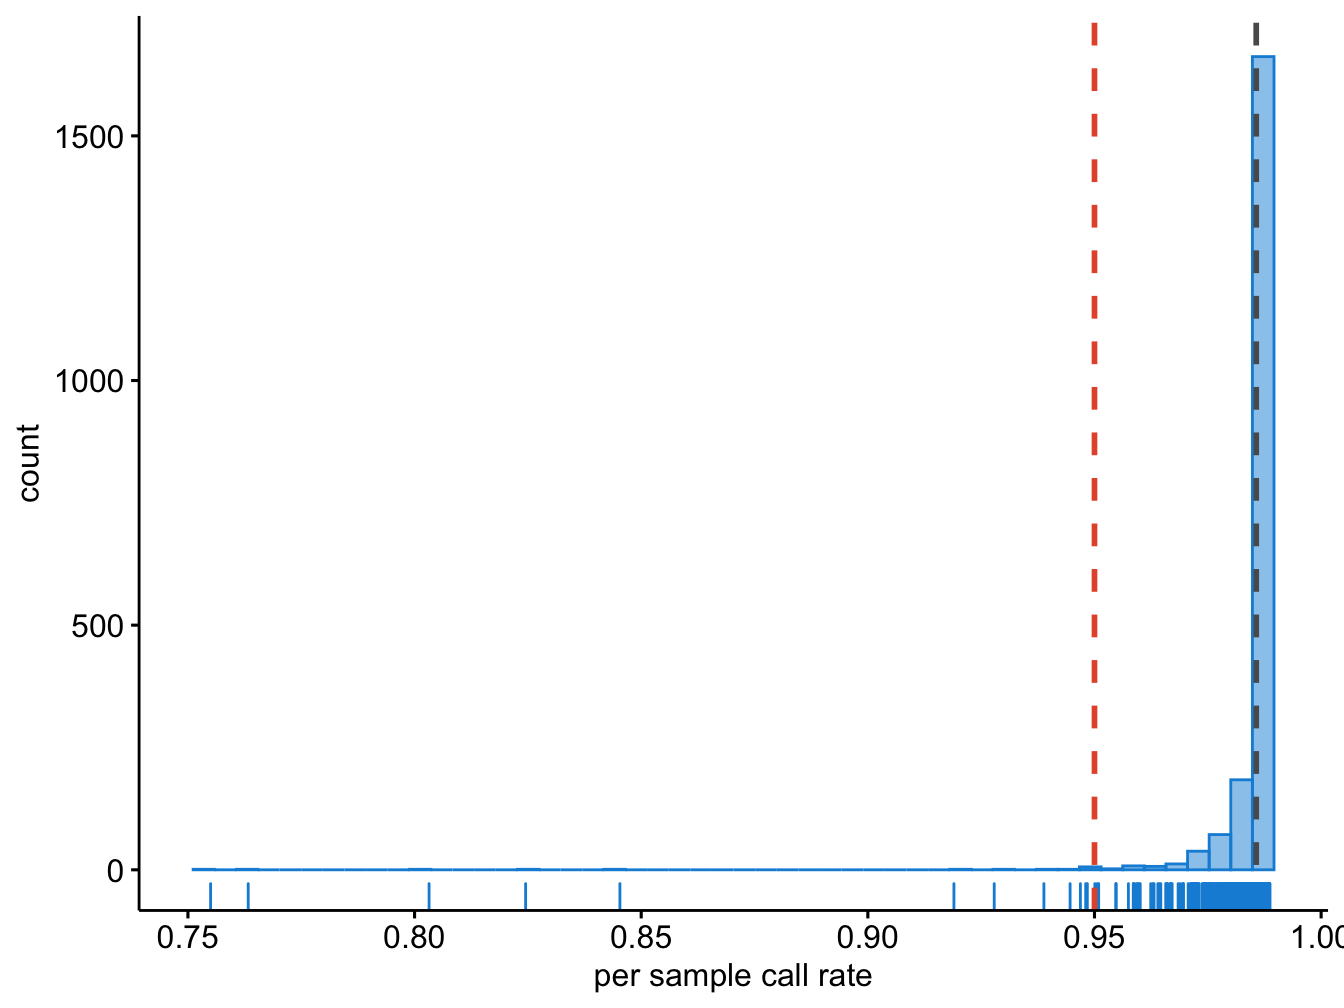
\includegraphics[width=0.85\linewidth]{img/_gwas_dummy/gwas-qc-sample-callrate} 

}

\caption{Per sample call rate.}\label{fig:showsamplecallrate}
\end{figure}

\hypertarget{heterozygosity-rate}{%
\section{Heterozygosity rate}\label{heterozygosity-rate}}

To properly calculate heterozygosity rate and relatedness (identity-by-descent {[}IBD{]}) we need to do four things:

\begin{enumerate}
\def\labelenumi{\arabic{enumi})}
\tightlist
\item
  pre-clean the data to get a high-quality set,
\item
  of independent SNPs,
\item
  exclude long-range linkage disequilibrium (LD) blocks that bias with these calculations, and
\item
  exclude A/T and C/G SNPs as these may be ambivalent in interpretation when frequencies between cases and controls are close (MAF ± 0.45),
\item
  remove all non-autosomal SNPs.
\end{enumerate}

You can find an up-to-date list of LD blocks you should exclude in these types of analyses \href{https://genome.sph.umich.edu/wiki/Regions_of_high_linkage_disequilibrium_(LD)}{here} for the different genome builds. In this case we are using build 37. For the purpose of this book we included a file with these regions in the \passthrough{\lstinline!support!}-directory.

We will use the following settings:

\begin{itemize}
\tightlist
\item
  remove A/T and C/G SNPs with the flag \passthrough{\lstinline!--exclude dummy\_project/all.atcg.variants.txt!},
\item
  call rate \textless1\% with the flag \passthrough{\lstinline!--geno 0.10!},
\item
  Hardy-Weinberg Equilibrium (HWE) p-value \textgreater{} 1x10-3 with the flag \passthrough{\lstinline!--hwe 1e-3!},
\item
  and MAF\textgreater10\% with the flag \passthrough{\lstinline!--maf 0.10!},
\item
  prune the data to only select independent SNPs (with low LD r\^{}2) of one pair each with \passthrough{\lstinline!r\^2 = 0.2!} with the flags \passthrough{\lstinline!--indep-pairwise 100 10 0.2!} and \passthrough{\lstinline!--extract rawdata/raw-GWA-data.prune.in!},
\item
  SNPs in long-range LD regions (for example: MHC chr 6 25.8-36Mb, chr 8 inversion 6-16Mb, chr17 40-45Mb, and a few more) with the flag \passthrough{\lstinline!--exclude range support/exclude\_problematic\_range.txt!},
\item
  remove non-autosomal SNPs with the flag \passthrough{\lstinline!--autosome!}.
\end{itemize}

First, get a list of A/T and C/G SNPs. Remember, the list of markers for this GWAS is noted in the \passthrough{\lstinline!.bim!} file. We can simply grep all the lines where the two alleles either have an A/T or C/G combination.

\begin{lstlisting}
cat dummy_project/rawdata.bim | \
awk '($5 == "A" && $6 == "T") || ($5 == "T" && $6 == "A") || ($5 == "C" && $6 == "G") || ($5 == "G" && $6 == "C")' | awk '{ print $2, $1, $4, $3, $5, $6 }' \
> dummy_project/all.atcg.variants.txt
\end{lstlisting}

Second, clean the data and get a list of independent SNPs.

\begin{lstlisting}
plink --bfile dummy_project/rawdata \
--autosome \
--maf 0.10 --geno 0.10 --hwe 1e-3 \
--indep-pairwise 100 10 0.2 \
--exclude range support/exclude_problematic_range.txt \
--make-bed --out dummy_project/rawdata.clean.temp
\end{lstlisting}

\begin{quote}
Please note, we have create a dataset without taking into account LD structure. Hence, the message `Pruned 0 variants from chromosome 1, leaving 19420.' etc. In a dataset without any LD structure this flag \passthrough{\lstinline!--indep-pairwise 100 10 0.2!} doesn't actually work. However, with real-data you can use it to prune out unwanted SNPs in high LD.
\end{quote}

Third, exclude the pruned SNPs. Note, how we include a file to exclude high-LD for the purpose of the practical.

\begin{lstlisting}
plink --bfile dummy_project/rawdata.clean.temp \
--extract rawdata/raw-GWA-data.prune.in \
--make-bed --out dummy_project/rawdata.clean.ultraclean.temp
\end{lstlisting}

Fourth, remove the A/T and C/G SNPs.

\begin{lstlisting}
plink --bfile dummy_project/rawdata.clean.ultraclean.temp \
--exclude dummy_project/all.atcg.variants.txt \
--make-bed --out dummy_project/rawdata.clean.ultraclean
\end{lstlisting}

\begin{quote}
Please note, this dataset doesn't actually include this type of SNP, hence \passthrough{\lstinline!rawdata/all.atcg.variants.txt!} is empty! Again, you can use this command in real-data to exclude A/T and C/G SNPs.
\end{quote}

Lastly, remove the temporary files.

\begin{lstlisting}
rm -fv dummy_project/*.temp*
\end{lstlisting}

Finally, we can calculate the heterozygosity rate.

\begin{lstlisting}
plink --bfile dummy_project/rawdata.clean.ultraclean --het --out dummy_project/rawdata.clean.ultraclean
\end{lstlisting}

This creates the file \passthrough{\lstinline!dummy\_project/rawdata.clean.ultraclean.het!}, in which the third column denotes the observed number of homozygous genotypes, O(Hom), and the fifth column denotes the number of nonmissing genotypes, N(NM), per individual. We can now calculate the observed heterozygosity rate per individual using the formula (N(NM) - O(Hom))/N(NM).

Often there is a correlation between heterozygosity rate and missing data. Thus, we should plot the observed heterozygosity rate per individual on the x-axis and the proportion of missing SNP, that is the `SNP call rate', per individuals on the y-axis (Figure \ref{fig:showheterozygosity}).

\begin{figure}[H]

{\centering 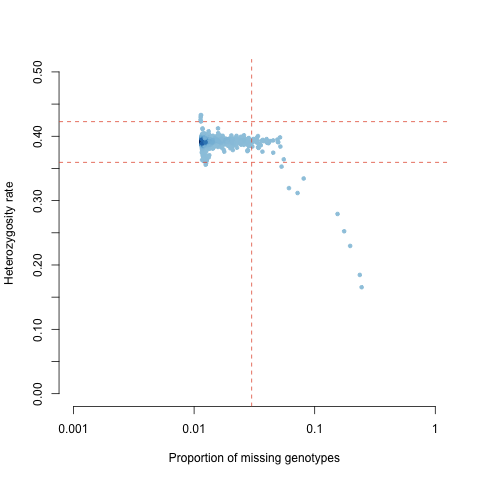
\includegraphics[width=0.85\linewidth]{img/_gwas_dummy/show-heterozygosity} 

}

\caption{Heterozygosity as a function of SNP call rate.}\label{fig:showheterozygosity}
\end{figure}

Examine the plot (Figure \ref{fig:showheterozygosity}) to decide reasonable thresholds at which to exclude individuals based on elevated missing or extreme heterozygosity. We chose to exclude all individuals with a genotype failure rate \textgreater= 0.03 (vertical dashed line) and/or a heterozygosity rate ± 3 s.d. from the mean (horizontal dashed lines). Add the FID and IID of the samples failing this QC to the file named \passthrough{\lstinline!fail-imisshet-qc.txt!}.

\begin{quote}
How would you create this file?
\end{quote}

If all is right, you'd have something like Table \ref{tab:failedcallratehet}.

\global\setlength{\Oldarrayrulewidth}{\arrayrulewidth}

\global\setlength{\Oldtabcolsep}{\tabcolsep}

\setlength{\tabcolsep}{2pt}

\renewcommand*{\arraystretch}{1.5}



\providecommand{\ascline}[3]{\noalign{\global\arrayrulewidth #1}\arrayrulecolor[HTML]{#2}\cline{#3}}

\begin{longtable}[c]{|p{0.57in}|p{0.57in}}

\caption{Failed\ samples\ due\ to\ sample\ call\ rates\ and\ heterozygosity\ rate.}\label{tab:failedcallratehet}\\

\ascline{1.5pt}{666666}{1-2}

\multicolumn{1}{>{\raggedleft}m{\dimexpr 0.57in+0\tabcolsep}}{\textcolor[HTML]{000000}{\fontsize{11}{11}\selectfont{\global\setmainfont{Helvetica}{FID}}}} & \multicolumn{1}{>{\raggedleft}m{\dimexpr 0.57in+0\tabcolsep}}{\textcolor[HTML]{000000}{\fontsize{11}{11}\selectfont{\global\setmainfont{Helvetica}{IID}}}} \\

\ascline{1.5pt}{666666}{1-2}\endfirsthead \caption[]{Failed\ samples\ due\ to\ sample\ call\ rates\ and\ heterozygosity\ rate.}\label{tab:failedcallratehet}\\

\ascline{1.5pt}{666666}{1-2}

\multicolumn{1}{>{\raggedleft}m{\dimexpr 0.57in+0\tabcolsep}}{\textcolor[HTML]{000000}{\fontsize{11}{11}\selectfont{\global\setmainfont{Helvetica}{FID}}}} & \multicolumn{1}{>{\raggedleft}m{\dimexpr 0.57in+0\tabcolsep}}{\textcolor[HTML]{000000}{\fontsize{11}{11}\selectfont{\global\setmainfont{Helvetica}{IID}}}} \\

\ascline{1.5pt}{666666}{1-2}\endhead



\multicolumn{1}{>{\raggedleft}m{\dimexpr 0.57in+0\tabcolsep}}{\textcolor[HTML]{000000}{\fontsize{11}{11}\selectfont{\global\setmainfont{Helvetica}{28}}}} & \multicolumn{1}{>{\raggedleft}m{\dimexpr 0.57in+0\tabcolsep}}{\textcolor[HTML]{000000}{\fontsize{11}{11}\selectfont{\global\setmainfont{Helvetica}{28}}}} \\





\multicolumn{1}{>{\raggedleft}m{\dimexpr 0.57in+0\tabcolsep}}{\textcolor[HTML]{000000}{\fontsize{11}{11}\selectfont{\global\setmainfont{Helvetica}{50}}}} & \multicolumn{1}{>{\raggedleft}m{\dimexpr 0.57in+0\tabcolsep}}{\textcolor[HTML]{000000}{\fontsize{11}{11}\selectfont{\global\setmainfont{Helvetica}{50}}}} \\





\multicolumn{1}{>{\raggedleft}m{\dimexpr 0.57in+0\tabcolsep}}{\textcolor[HTML]{000000}{\fontsize{11}{11}\selectfont{\global\setmainfont{Helvetica}{52}}}} & \multicolumn{1}{>{\raggedleft}m{\dimexpr 0.57in+0\tabcolsep}}{\textcolor[HTML]{000000}{\fontsize{11}{11}\selectfont{\global\setmainfont{Helvetica}{52}}}} \\





\multicolumn{1}{>{\raggedleft}m{\dimexpr 0.57in+0\tabcolsep}}{\textcolor[HTML]{000000}{\fontsize{11}{11}\selectfont{\global\setmainfont{Helvetica}{53}}}} & \multicolumn{1}{>{\raggedleft}m{\dimexpr 0.57in+0\tabcolsep}}{\textcolor[HTML]{000000}{\fontsize{11}{11}\selectfont{\global\setmainfont{Helvetica}{53}}}} \\





\multicolumn{1}{>{\raggedleft}m{\dimexpr 0.57in+0\tabcolsep}}{\textcolor[HTML]{000000}{\fontsize{11}{11}\selectfont{\global\setmainfont{Helvetica}{67}}}} & \multicolumn{1}{>{\raggedleft}m{\dimexpr 0.57in+0\tabcolsep}}{\textcolor[HTML]{000000}{\fontsize{11}{11}\selectfont{\global\setmainfont{Helvetica}{67}}}} \\





\multicolumn{1}{>{\raggedleft}m{\dimexpr 0.57in+0\tabcolsep}}{\textcolor[HTML]{000000}{\fontsize{11}{11}\selectfont{\global\setmainfont{Helvetica}{96}}}} & \multicolumn{1}{>{\raggedleft}m{\dimexpr 0.57in+0\tabcolsep}}{\textcolor[HTML]{000000}{\fontsize{11}{11}\selectfont{\global\setmainfont{Helvetica}{96}}}} \\





\multicolumn{1}{>{\raggedleft}m{\dimexpr 0.57in+0\tabcolsep}}{\textcolor[HTML]{000000}{\fontsize{11}{11}\selectfont{\global\setmainfont{Helvetica}{205}}}} & \multicolumn{1}{>{\raggedleft}m{\dimexpr 0.57in+0\tabcolsep}}{\textcolor[HTML]{000000}{\fontsize{11}{11}\selectfont{\global\setmainfont{Helvetica}{205}}}} \\





\multicolumn{1}{>{\raggedleft}m{\dimexpr 0.57in+0\tabcolsep}}{\textcolor[HTML]{000000}{\fontsize{11}{11}\selectfont{\global\setmainfont{Helvetica}{298}}}} & \multicolumn{1}{>{\raggedleft}m{\dimexpr 0.57in+0\tabcolsep}}{\textcolor[HTML]{000000}{\fontsize{11}{11}\selectfont{\global\setmainfont{Helvetica}{298}}}} \\





\multicolumn{1}{>{\raggedleft}m{\dimexpr 0.57in+0\tabcolsep}}{\textcolor[HTML]{000000}{\fontsize{11}{11}\selectfont{\global\setmainfont{Helvetica}{310}}}} & \multicolumn{1}{>{\raggedleft}m{\dimexpr 0.57in+0\tabcolsep}}{\textcolor[HTML]{000000}{\fontsize{11}{11}\selectfont{\global\setmainfont{Helvetica}{310}}}} \\





\multicolumn{1}{>{\raggedleft}m{\dimexpr 0.57in+0\tabcolsep}}{\textcolor[HTML]{000000}{\fontsize{11}{11}\selectfont{\global\setmainfont{Helvetica}{351}}}} & \multicolumn{1}{>{\raggedleft}m{\dimexpr 0.57in+0\tabcolsep}}{\textcolor[HTML]{000000}{\fontsize{11}{11}\selectfont{\global\setmainfont{Helvetica}{351}}}} \\





\multicolumn{1}{>{\raggedleft}m{\dimexpr 0.57in+0\tabcolsep}}{\textcolor[HTML]{000000}{\fontsize{11}{11}\selectfont{\global\setmainfont{Helvetica}{404}}}} & \multicolumn{1}{>{\raggedleft}m{\dimexpr 0.57in+0\tabcolsep}}{\textcolor[HTML]{000000}{\fontsize{11}{11}\selectfont{\global\setmainfont{Helvetica}{404}}}} \\





\multicolumn{1}{>{\raggedleft}m{\dimexpr 0.57in+0\tabcolsep}}{\textcolor[HTML]{000000}{\fontsize{11}{11}\selectfont{\global\setmainfont{Helvetica}{418}}}} & \multicolumn{1}{>{\raggedleft}m{\dimexpr 0.57in+0\tabcolsep}}{\textcolor[HTML]{000000}{\fontsize{11}{11}\selectfont{\global\setmainfont{Helvetica}{418}}}} \\





\multicolumn{1}{>{\raggedleft}m{\dimexpr 0.57in+0\tabcolsep}}{\textcolor[HTML]{000000}{\fontsize{11}{11}\selectfont{\global\setmainfont{Helvetica}{423}}}} & \multicolumn{1}{>{\raggedleft}m{\dimexpr 0.57in+0\tabcolsep}}{\textcolor[HTML]{000000}{\fontsize{11}{11}\selectfont{\global\setmainfont{Helvetica}{423}}}} \\





\multicolumn{1}{>{\raggedleft}m{\dimexpr 0.57in+0\tabcolsep}}{\textcolor[HTML]{000000}{\fontsize{11}{11}\selectfont{\global\setmainfont{Helvetica}{428}}}} & \multicolumn{1}{>{\raggedleft}m{\dimexpr 0.57in+0\tabcolsep}}{\textcolor[HTML]{000000}{\fontsize{11}{11}\selectfont{\global\setmainfont{Helvetica}{428}}}} \\





\multicolumn{1}{>{\raggedleft}m{\dimexpr 0.57in+0\tabcolsep}}{\textcolor[HTML]{000000}{\fontsize{11}{11}\selectfont{\global\setmainfont{Helvetica}{442}}}} & \multicolumn{1}{>{\raggedleft}m{\dimexpr 0.57in+0\tabcolsep}}{\textcolor[HTML]{000000}{\fontsize{11}{11}\selectfont{\global\setmainfont{Helvetica}{442}}}} \\





\multicolumn{1}{>{\raggedleft}m{\dimexpr 0.57in+0\tabcolsep}}{\textcolor[HTML]{000000}{\fontsize{11}{11}\selectfont{\global\setmainfont{Helvetica}{444}}}} & \multicolumn{1}{>{\raggedleft}m{\dimexpr 0.57in+0\tabcolsep}}{\textcolor[HTML]{000000}{\fontsize{11}{11}\selectfont{\global\setmainfont{Helvetica}{444}}}} \\





\multicolumn{1}{>{\raggedleft}m{\dimexpr 0.57in+0\tabcolsep}}{\textcolor[HTML]{000000}{\fontsize{11}{11}\selectfont{\global\setmainfont{Helvetica}{548}}}} & \multicolumn{1}{>{\raggedleft}m{\dimexpr 0.57in+0\tabcolsep}}{\textcolor[HTML]{000000}{\fontsize{11}{11}\selectfont{\global\setmainfont{Helvetica}{548}}}} \\





\multicolumn{1}{>{\raggedleft}m{\dimexpr 0.57in+0\tabcolsep}}{\textcolor[HTML]{000000}{\fontsize{11}{11}\selectfont{\global\setmainfont{Helvetica}{772}}}} & \multicolumn{1}{>{\raggedleft}m{\dimexpr 0.57in+0\tabcolsep}}{\textcolor[HTML]{000000}{\fontsize{11}{11}\selectfont{\global\setmainfont{Helvetica}{772}}}} \\





\multicolumn{1}{>{\raggedleft}m{\dimexpr 0.57in+0\tabcolsep}}{\textcolor[HTML]{000000}{\fontsize{11}{11}\selectfont{\global\setmainfont{Helvetica}{835}}}} & \multicolumn{1}{>{\raggedleft}m{\dimexpr 0.57in+0\tabcolsep}}{\textcolor[HTML]{000000}{\fontsize{11}{11}\selectfont{\global\setmainfont{Helvetica}{835}}}} \\





\multicolumn{1}{>{\raggedleft}m{\dimexpr 0.57in+0\tabcolsep}}{\textcolor[HTML]{000000}{\fontsize{11}{11}\selectfont{\global\setmainfont{Helvetica}{850}}}} & \multicolumn{1}{>{\raggedleft}m{\dimexpr 0.57in+0\tabcolsep}}{\textcolor[HTML]{000000}{\fontsize{11}{11}\selectfont{\global\setmainfont{Helvetica}{850}}}} \\





\multicolumn{1}{>{\raggedleft}m{\dimexpr 0.57in+0\tabcolsep}}{\textcolor[HTML]{000000}{\fontsize{11}{11}\selectfont{\global\setmainfont{Helvetica}{853}}}} & \multicolumn{1}{>{\raggedleft}m{\dimexpr 0.57in+0\tabcolsep}}{\textcolor[HTML]{000000}{\fontsize{11}{11}\selectfont{\global\setmainfont{Helvetica}{853}}}} \\





\multicolumn{1}{>{\raggedleft}m{\dimexpr 0.57in+0\tabcolsep}}{\textcolor[HTML]{000000}{\fontsize{11}{11}\selectfont{\global\setmainfont{Helvetica}{910}}}} & \multicolumn{1}{>{\raggedleft}m{\dimexpr 0.57in+0\tabcolsep}}{\textcolor[HTML]{000000}{\fontsize{11}{11}\selectfont{\global\setmainfont{Helvetica}{910}}}} \\





\multicolumn{1}{>{\raggedleft}m{\dimexpr 0.57in+0\tabcolsep}}{\textcolor[HTML]{000000}{\fontsize{11}{11}\selectfont{\global\setmainfont{Helvetica}{939}}}} & \multicolumn{1}{>{\raggedleft}m{\dimexpr 0.57in+0\tabcolsep}}{\textcolor[HTML]{000000}{\fontsize{11}{11}\selectfont{\global\setmainfont{Helvetica}{939}}}} \\





\multicolumn{1}{>{\raggedleft}m{\dimexpr 0.57in+0\tabcolsep}}{\textcolor[HTML]{000000}{\fontsize{11}{11}\selectfont{\global\setmainfont{Helvetica}{966}}}} & \multicolumn{1}{>{\raggedleft}m{\dimexpr 0.57in+0\tabcolsep}}{\textcolor[HTML]{000000}{\fontsize{11}{11}\selectfont{\global\setmainfont{Helvetica}{966}}}} \\





\multicolumn{1}{>{\raggedleft}m{\dimexpr 0.57in+0\tabcolsep}}{\textcolor[HTML]{000000}{\fontsize{11}{11}\selectfont{\global\setmainfont{Helvetica}{968}}}} & \multicolumn{1}{>{\raggedleft}m{\dimexpr 0.57in+0\tabcolsep}}{\textcolor[HTML]{000000}{\fontsize{11}{11}\selectfont{\global\setmainfont{Helvetica}{968}}}} \\





\multicolumn{1}{>{\raggedleft}m{\dimexpr 0.57in+0\tabcolsep}}{\textcolor[HTML]{000000}{\fontsize{11}{11}\selectfont{\global\setmainfont{Helvetica}{1,003}}}} & \multicolumn{1}{>{\raggedleft}m{\dimexpr 0.57in+0\tabcolsep}}{\textcolor[HTML]{000000}{\fontsize{11}{11}\selectfont{\global\setmainfont{Helvetica}{1,003}}}} \\





\multicolumn{1}{>{\raggedleft}m{\dimexpr 0.57in+0\tabcolsep}}{\textcolor[HTML]{000000}{\fontsize{11}{11}\selectfont{\global\setmainfont{Helvetica}{1,006}}}} & \multicolumn{1}{>{\raggedleft}m{\dimexpr 0.57in+0\tabcolsep}}{\textcolor[HTML]{000000}{\fontsize{11}{11}\selectfont{\global\setmainfont{Helvetica}{1,006}}}} \\





\multicolumn{1}{>{\raggedleft}m{\dimexpr 0.57in+0\tabcolsep}}{\textcolor[HTML]{000000}{\fontsize{11}{11}\selectfont{\global\setmainfont{Helvetica}{1,045}}}} & \multicolumn{1}{>{\raggedleft}m{\dimexpr 0.57in+0\tabcolsep}}{\textcolor[HTML]{000000}{\fontsize{11}{11}\selectfont{\global\setmainfont{Helvetica}{1,045}}}} \\





\multicolumn{1}{>{\raggedleft}m{\dimexpr 0.57in+0\tabcolsep}}{\textcolor[HTML]{000000}{\fontsize{11}{11}\selectfont{\global\setmainfont{Helvetica}{1,058}}}} & \multicolumn{1}{>{\raggedleft}m{\dimexpr 0.57in+0\tabcolsep}}{\textcolor[HTML]{000000}{\fontsize{11}{11}\selectfont{\global\setmainfont{Helvetica}{1,058}}}} \\





\multicolumn{1}{>{\raggedleft}m{\dimexpr 0.57in+0\tabcolsep}}{\textcolor[HTML]{000000}{\fontsize{11}{11}\selectfont{\global\setmainfont{Helvetica}{1,154}}}} & \multicolumn{1}{>{\raggedleft}m{\dimexpr 0.57in+0\tabcolsep}}{\textcolor[HTML]{000000}{\fontsize{11}{11}\selectfont{\global\setmainfont{Helvetica}{1,154}}}} \\





\multicolumn{1}{>{\raggedleft}m{\dimexpr 0.57in+0\tabcolsep}}{\textcolor[HTML]{000000}{\fontsize{11}{11}\selectfont{\global\setmainfont{Helvetica}{1,236}}}} & \multicolumn{1}{>{\raggedleft}m{\dimexpr 0.57in+0\tabcolsep}}{\textcolor[HTML]{000000}{\fontsize{11}{11}\selectfont{\global\setmainfont{Helvetica}{1,236}}}} \\





\multicolumn{1}{>{\raggedleft}m{\dimexpr 0.57in+0\tabcolsep}}{\textcolor[HTML]{000000}{\fontsize{11}{11}\selectfont{\global\setmainfont{Helvetica}{1,294}}}} & \multicolumn{1}{>{\raggedleft}m{\dimexpr 0.57in+0\tabcolsep}}{\textcolor[HTML]{000000}{\fontsize{11}{11}\selectfont{\global\setmainfont{Helvetica}{1,294}}}} \\





\multicolumn{1}{>{\raggedleft}m{\dimexpr 0.57in+0\tabcolsep}}{\textcolor[HTML]{000000}{\fontsize{11}{11}\selectfont{\global\setmainfont{Helvetica}{1,395}}}} & \multicolumn{1}{>{\raggedleft}m{\dimexpr 0.57in+0\tabcolsep}}{\textcolor[HTML]{000000}{\fontsize{11}{11}\selectfont{\global\setmainfont{Helvetica}{1,395}}}} \\





\multicolumn{1}{>{\raggedleft}m{\dimexpr 0.57in+0\tabcolsep}}{\textcolor[HTML]{000000}{\fontsize{11}{11}\selectfont{\global\setmainfont{Helvetica}{1,537}}}} & \multicolumn{1}{>{\raggedleft}m{\dimexpr 0.57in+0\tabcolsep}}{\textcolor[HTML]{000000}{\fontsize{11}{11}\selectfont{\global\setmainfont{Helvetica}{1,537}}}} \\





\multicolumn{1}{>{\raggedleft}m{\dimexpr 0.57in+0\tabcolsep}}{\textcolor[HTML]{000000}{\fontsize{11}{11}\selectfont{\global\setmainfont{Helvetica}{1,554}}}} & \multicolumn{1}{>{\raggedleft}m{\dimexpr 0.57in+0\tabcolsep}}{\textcolor[HTML]{000000}{\fontsize{11}{11}\selectfont{\global\setmainfont{Helvetica}{1,554}}}} \\





\multicolumn{1}{>{\raggedleft}m{\dimexpr 0.57in+0\tabcolsep}}{\textcolor[HTML]{000000}{\fontsize{11}{11}\selectfont{\global\setmainfont{Helvetica}{1,587}}}} & \multicolumn{1}{>{\raggedleft}m{\dimexpr 0.57in+0\tabcolsep}}{\textcolor[HTML]{000000}{\fontsize{11}{11}\selectfont{\global\setmainfont{Helvetica}{1,587}}}} \\





\multicolumn{1}{>{\raggedleft}m{\dimexpr 0.57in+0\tabcolsep}}{\textcolor[HTML]{000000}{\fontsize{11}{11}\selectfont{\global\setmainfont{Helvetica}{1,694}}}} & \multicolumn{1}{>{\raggedleft}m{\dimexpr 0.57in+0\tabcolsep}}{\textcolor[HTML]{000000}{\fontsize{11}{11}\selectfont{\global\setmainfont{Helvetica}{1,694}}}} \\





\multicolumn{1}{>{\raggedleft}m{\dimexpr 0.57in+0\tabcolsep}}{\textcolor[HTML]{000000}{\fontsize{11}{11}\selectfont{\global\setmainfont{Helvetica}{1,789}}}} & \multicolumn{1}{>{\raggedleft}m{\dimexpr 0.57in+0\tabcolsep}}{\textcolor[HTML]{000000}{\fontsize{11}{11}\selectfont{\global\setmainfont{Helvetica}{1,789}}}} \\





\multicolumn{1}{>{\raggedleft}m{\dimexpr 0.57in+0\tabcolsep}}{\textcolor[HTML]{000000}{\fontsize{11}{11}\selectfont{\global\setmainfont{Helvetica}{1,832}}}} & \multicolumn{1}{>{\raggedleft}m{\dimexpr 0.57in+0\tabcolsep}}{\textcolor[HTML]{000000}{\fontsize{11}{11}\selectfont{\global\setmainfont{Helvetica}{1,832}}}} \\





\multicolumn{1}{>{\raggedleft}m{\dimexpr 0.57in+0\tabcolsep}}{\textcolor[HTML]{000000}{\fontsize{11}{11}\selectfont{\global\setmainfont{Helvetica}{1,866}}}} & \multicolumn{1}{>{\raggedleft}m{\dimexpr 0.57in+0\tabcolsep}}{\textcolor[HTML]{000000}{\fontsize{11}{11}\selectfont{\global\setmainfont{Helvetica}{1,866}}}} \\





\multicolumn{1}{>{\raggedleft}m{\dimexpr 0.57in+0\tabcolsep}}{\textcolor[HTML]{000000}{\fontsize{11}{11}\selectfont{\global\setmainfont{Helvetica}{1,904}}}} & \multicolumn{1}{>{\raggedleft}m{\dimexpr 0.57in+0\tabcolsep}}{\textcolor[HTML]{000000}{\fontsize{11}{11}\selectfont{\global\setmainfont{Helvetica}{1,904}}}} \\





\multicolumn{1}{>{\raggedleft}m{\dimexpr 0.57in+0\tabcolsep}}{\textcolor[HTML]{000000}{\fontsize{11}{11}\selectfont{\global\setmainfont{Helvetica}{1,920}}}} & \multicolumn{1}{>{\raggedleft}m{\dimexpr 0.57in+0\tabcolsep}}{\textcolor[HTML]{000000}{\fontsize{11}{11}\selectfont{\global\setmainfont{Helvetica}{1,920}}}} \\





\multicolumn{1}{>{\raggedleft}m{\dimexpr 0.57in+0\tabcolsep}}{\textcolor[HTML]{000000}{\fontsize{11}{11}\selectfont{\global\setmainfont{Helvetica}{1,951}}}} & \multicolumn{1}{>{\raggedleft}m{\dimexpr 0.57in+0\tabcolsep}}{\textcolor[HTML]{000000}{\fontsize{11}{11}\selectfont{\global\setmainfont{Helvetica}{1,951}}}} \\





\multicolumn{1}{>{\raggedleft}m{\dimexpr 0.57in+0\tabcolsep}}{\textcolor[HTML]{000000}{\fontsize{11}{11}\selectfont{\global\setmainfont{Helvetica}{1,952}}}} & \multicolumn{1}{>{\raggedleft}m{\dimexpr 0.57in+0\tabcolsep}}{\textcolor[HTML]{000000}{\fontsize{11}{11}\selectfont{\global\setmainfont{Helvetica}{1,952}}}} \\





\multicolumn{1}{>{\raggedleft}m{\dimexpr 0.57in+0\tabcolsep}}{\textcolor[HTML]{000000}{\fontsize{11}{11}\selectfont{\global\setmainfont{Helvetica}{1,953}}}} & \multicolumn{1}{>{\raggedleft}m{\dimexpr 0.57in+0\tabcolsep}}{\textcolor[HTML]{000000}{\fontsize{11}{11}\selectfont{\global\setmainfont{Helvetica}{1,953}}}} \\





\multicolumn{1}{>{\raggedleft}m{\dimexpr 0.57in+0\tabcolsep}}{\textcolor[HTML]{000000}{\fontsize{11}{11}\selectfont{\global\setmainfont{Helvetica}{1,954}}}} & \multicolumn{1}{>{\raggedleft}m{\dimexpr 0.57in+0\tabcolsep}}{\textcolor[HTML]{000000}{\fontsize{11}{11}\selectfont{\global\setmainfont{Helvetica}{1,954}}}} \\





\multicolumn{1}{>{\raggedleft}m{\dimexpr 0.57in+0\tabcolsep}}{\textcolor[HTML]{000000}{\fontsize{11}{11}\selectfont{\global\setmainfont{Helvetica}{1,955}}}} & \multicolumn{1}{>{\raggedleft}m{\dimexpr 0.57in+0\tabcolsep}}{\textcolor[HTML]{000000}{\fontsize{11}{11}\selectfont{\global\setmainfont{Helvetica}{1,955}}}} \\





\multicolumn{1}{>{\raggedleft}m{\dimexpr 0.57in+0\tabcolsep}}{\textcolor[HTML]{000000}{\fontsize{11}{11}\selectfont{\global\setmainfont{Helvetica}{1,981}}}} & \multicolumn{1}{>{\raggedleft}m{\dimexpr 0.57in+0\tabcolsep}}{\textcolor[HTML]{000000}{\fontsize{11}{11}\selectfont{\global\setmainfont{Helvetica}{1,981}}}} \\





\multicolumn{1}{>{\raggedleft}m{\dimexpr 0.57in+0\tabcolsep}}{\textcolor[HTML]{000000}{\fontsize{11}{11}\selectfont{\global\setmainfont{Helvetica}{1,984}}}} & \multicolumn{1}{>{\raggedleft}m{\dimexpr 0.57in+0\tabcolsep}}{\textcolor[HTML]{000000}{\fontsize{11}{11}\selectfont{\global\setmainfont{Helvetica}{1,984}}}} \\





\multicolumn{1}{>{\raggedleft}m{\dimexpr 0.57in+0\tabcolsep}}{\textcolor[HTML]{000000}{\fontsize{11}{11}\selectfont{\global\setmainfont{Helvetica}{1,985}}}} & \multicolumn{1}{>{\raggedleft}m{\dimexpr 0.57in+0\tabcolsep}}{\textcolor[HTML]{000000}{\fontsize{11}{11}\selectfont{\global\setmainfont{Helvetica}{1,985}}}} \\





\multicolumn{1}{>{\raggedleft}m{\dimexpr 0.57in+0\tabcolsep}}{\textcolor[HTML]{000000}{\fontsize{11}{11}\selectfont{\global\setmainfont{Helvetica}{1,986}}}} & \multicolumn{1}{>{\raggedleft}m{\dimexpr 0.57in+0\tabcolsep}}{\textcolor[HTML]{000000}{\fontsize{11}{11}\selectfont{\global\setmainfont{Helvetica}{1,986}}}} \\

\ascline{1.5pt}{666666}{1-2}



\end{longtable}



\arrayrulecolor[HTML]{000000}

\global\setlength{\arrayrulewidth}{\Oldarrayrulewidth}

\global\setlength{\tabcolsep}{\Oldtabcolsep}

\renewcommand*{\arraystretch}{1}

\hypertarget{relatedness}{%
\section{Relatedness}\label{relatedness}}

We calculate Identity-by-Descent (IBS) to identify duplicated and related samples. In Table \ref{tab:showrelatedness} we show how much DNA is shared between individuals depending on their relation\citep{staples2014}. IBS is measured by calculating pi-hat (\(\widehat{\pi}\)), which is in essence the proportion of the DNA that a pair of samples share. To calculate this, we needed this ultraclean dataset, without low-quality SNPs and without high-LD regions.

\global\setlength{\Oldarrayrulewidth}{\arrayrulewidth}

\global\setlength{\Oldtabcolsep}{\tabcolsep}

\setlength{\tabcolsep}{2pt}

\renewcommand*{\arraystretch}{1.5}



\providecommand{\ascline}[3]{\noalign{\global\arrayrulewidth #1}\arrayrulecolor[HTML]{#2}\cline{#3}}

\begin{longtable}[c]{|p{4.11in}|p{1.23in}|p{0.74in}|p{0.81in}|p{0.52in}}

\caption{Familial\ relations\ and\ \%\ DNA\ shared.}\label{tab:showrelatedness}\\

\ascline{1.5pt}{666666}{1-5}

\multicolumn{1}{>{\raggedright}m{\dimexpr 4.11in+0\tabcolsep}}{\textcolor[HTML]{000000}{\fontsize{11}{11}\selectfont{\global\setmainfont{Helvetica}{Relatedness}}}} & \multicolumn{1}{>{\raggedright}m{\dimexpr 1.23in+0\tabcolsep}}{\textcolor[HTML]{000000}{\fontsize{11}{11}\selectfont{\global\setmainfont{Helvetica}{\%.DNA.sharing}}}} & \multicolumn{1}{>{\raggedright}m{\dimexpr 0.74in+0\tabcolsep}}{\textcolor[HTML]{000000}{\fontsize{11}{11}\selectfont{\global\setmainfont{Helvetica}{IBD0}}}} & \multicolumn{1}{>{\raggedright}m{\dimexpr 0.81in+0\tabcolsep}}{\textcolor[HTML]{000000}{\fontsize{11}{11}\selectfont{\global\setmainfont{Helvetica}{IBD1}}}} & \multicolumn{1}{>{\raggedleft}m{\dimexpr 0.52in+0\tabcolsep}}{\textcolor[HTML]{000000}{\fontsize{11}{11}\selectfont{\global\setmainfont{Helvetica}{IBD2}}}} \\

\ascline{1.5pt}{666666}{1-5}\endfirsthead \caption[]{Familial\ relations\ and\ \%\ DNA\ shared.}\label{tab:showrelatedness}\\

\ascline{1.5pt}{666666}{1-5}

\multicolumn{1}{>{\raggedright}m{\dimexpr 4.11in+0\tabcolsep}}{\textcolor[HTML]{000000}{\fontsize{11}{11}\selectfont{\global\setmainfont{Helvetica}{Relatedness}}}} & \multicolumn{1}{>{\raggedright}m{\dimexpr 1.23in+0\tabcolsep}}{\textcolor[HTML]{000000}{\fontsize{11}{11}\selectfont{\global\setmainfont{Helvetica}{\%.DNA.sharing}}}} & \multicolumn{1}{>{\raggedright}m{\dimexpr 0.74in+0\tabcolsep}}{\textcolor[HTML]{000000}{\fontsize{11}{11}\selectfont{\global\setmainfont{Helvetica}{IBD0}}}} & \multicolumn{1}{>{\raggedright}m{\dimexpr 0.81in+0\tabcolsep}}{\textcolor[HTML]{000000}{\fontsize{11}{11}\selectfont{\global\setmainfont{Helvetica}{IBD1}}}} & \multicolumn{1}{>{\raggedleft}m{\dimexpr 0.52in+0\tabcolsep}}{\textcolor[HTML]{000000}{\fontsize{11}{11}\selectfont{\global\setmainfont{Helvetica}{IBD2}}}} \\

\ascline{1.5pt}{666666}{1-5}\endhead



\multicolumn{1}{>{\raggedright}m{\dimexpr 4.11in+0\tabcolsep}}{\textcolor[HTML]{000000}{\fontsize{11}{11}\selectfont{\global\setmainfont{Helvetica}{Monozygotic\ twins\ \ \ \ \ \ \ \ \ \ }}}} & \multicolumn{1}{>{\raggedright}m{\dimexpr 1.23in+0\tabcolsep}}{\textcolor[HTML]{000000}{\fontsize{11}{11}\selectfont{\global\setmainfont{Helvetica}{\ ±100\%}}}} & \multicolumn{1}{>{\raggedright}m{\dimexpr 0.74in+0\tabcolsep}}{\textcolor[HTML]{000000}{\fontsize{11}{11}\selectfont{\global\setmainfont{Helvetica}{0}}}} & \multicolumn{1}{>{\raggedright}m{\dimexpr 0.81in+0\tabcolsep}}{\textcolor[HTML]{000000}{\fontsize{11}{11}\selectfont{\global\setmainfont{Helvetica}{1}}}} & \multicolumn{1}{>{\raggedleft}m{\dimexpr 0.52in+0\tabcolsep}}{\textcolor[HTML]{000000}{\fontsize{11}{11}\selectfont{\global\setmainfont{Helvetica}{0.00}}}} \\





\multicolumn{1}{>{\raggedright}m{\dimexpr 4.11in+0\tabcolsep}}{\textcolor[HTML]{000000}{\fontsize{11}{11}\selectfont{\global\setmainfont{Helvetica}{Parents/child\ \ \ \ \ \ \ \ \ \ \ \ \ \ }}}} & \multicolumn{1}{>{\raggedright}m{\dimexpr 1.23in+0\tabcolsep}}{\textcolor[HTML]{000000}{\fontsize{11}{11}\selectfont{\global\setmainfont{Helvetica}{\ ±50\%}}}} & \multicolumn{1}{>{\raggedright}m{\dimexpr 0.74in+0\tabcolsep}}{\textcolor[HTML]{000000}{\fontsize{11}{11}\selectfont{\global\setmainfont{Helvetica}{0.25}}}} & \multicolumn{1}{>{\raggedright}m{\dimexpr 0.81in+0\tabcolsep}}{\textcolor[HTML]{000000}{\fontsize{11}{11}\selectfont{\global\setmainfont{Helvetica}{0.5}}}} & \multicolumn{1}{>{\raggedleft}m{\dimexpr 0.52in+0\tabcolsep}}{\textcolor[HTML]{000000}{\fontsize{11}{11}\selectfont{\global\setmainfont{Helvetica}{0.25}}}} \\





\multicolumn{1}{>{\raggedright}m{\dimexpr 4.11in+0\tabcolsep}}{\textcolor[HTML]{000000}{\fontsize{11}{11}\selectfont{\global\setmainfont{Helvetica}{Sibling\ \ \ \ \ \ \ \ \ \ \ \ \ \ \ \ \ \ \ \ }}}} & \multicolumn{1}{>{\raggedright}m{\dimexpr 1.23in+0\tabcolsep}}{\textcolor[HTML]{000000}{\fontsize{11}{11}\selectfont{\global\setmainfont{Helvetica}{\ ±50\%}}}} & \multicolumn{1}{>{\raggedright}m{\dimexpr 0.74in+0\tabcolsep}}{\textcolor[HTML]{000000}{\fontsize{11}{11}\selectfont{\global\setmainfont{Helvetica}{0.25}}}} & \multicolumn{1}{>{\raggedright}m{\dimexpr 0.81in+0\tabcolsep}}{\textcolor[HTML]{000000}{\fontsize{11}{11}\selectfont{\global\setmainfont{Helvetica}{0.5}}}} & \multicolumn{1}{>{\raggedleft}m{\dimexpr 0.52in+0\tabcolsep}}{\textcolor[HTML]{000000}{\fontsize{11}{11}\selectfont{\global\setmainfont{Helvetica}{0.25}}}} \\





\multicolumn{1}{>{\raggedright}m{\dimexpr 4.11in+0\tabcolsep}}{\textcolor[HTML]{000000}{\fontsize{11}{11}\selectfont{\global\setmainfont{Helvetica}{Fraternal\ twins\ \ \ \ \ \ \ \ \ \ \ \ }}}} & \multicolumn{1}{>{\raggedright}m{\dimexpr 1.23in+0\tabcolsep}}{\textcolor[HTML]{000000}{\fontsize{11}{11}\selectfont{\global\setmainfont{Helvetica}{\ ±50\%}}}} & \multicolumn{1}{>{\raggedright}m{\dimexpr 0.74in+0\tabcolsep}}{\textcolor[HTML]{000000}{\fontsize{11}{11}\selectfont{\global\setmainfont{Helvetica}{0.25}}}} & \multicolumn{1}{>{\raggedright}m{\dimexpr 0.81in+0\tabcolsep}}{\textcolor[HTML]{000000}{\fontsize{11}{11}\selectfont{\global\setmainfont{Helvetica}{0.5}}}} & \multicolumn{1}{>{\raggedleft}m{\dimexpr 0.52in+0\tabcolsep}}{\textcolor[HTML]{000000}{\fontsize{11}{11}\selectfont{\global\setmainfont{Helvetica}{0.25}}}} \\





\multicolumn{1}{>{\raggedright}m{\dimexpr 4.11in+0\tabcolsep}}{\textcolor[HTML]{000000}{\fontsize{11}{11}\selectfont{\global\setmainfont{Helvetica}{Grandparent/grandchild\ \ \ \ \ }}}} & \multicolumn{1}{>{\raggedright}m{\dimexpr 1.23in+0\tabcolsep}}{\textcolor[HTML]{000000}{\fontsize{11}{11}\selectfont{\global\setmainfont{Helvetica}{\ ±25\%}}}} & \multicolumn{1}{>{\raggedright}m{\dimexpr 0.74in+0\tabcolsep}}{\textcolor[HTML]{000000}{\fontsize{11}{11}\selectfont{\global\setmainfont{Helvetica}{0.5}}}} & \multicolumn{1}{>{\raggedright}m{\dimexpr 0.81in+0\tabcolsep}}{\textcolor[HTML]{000000}{\fontsize{11}{11}\selectfont{\global\setmainfont{Helvetica}{0.5}}}} & \multicolumn{1}{>{\raggedleft}m{\dimexpr 0.52in+0\tabcolsep}}{\textcolor[HTML]{000000}{\fontsize{11}{11}\selectfont{\global\setmainfont{Helvetica}{0.00}}}} \\





\multicolumn{1}{>{\raggedright}m{\dimexpr 4.11in+0\tabcolsep}}{\textcolor[HTML]{000000}{\fontsize{11}{11}\selectfont{\global\setmainfont{Helvetica}{Aunt/Uncle/Niece/Nephew\ \ \ \ }}}} & \multicolumn{1}{>{\raggedright}m{\dimexpr 1.23in+0\tabcolsep}}{\textcolor[HTML]{000000}{\fontsize{11}{11}\selectfont{\global\setmainfont{Helvetica}{\ ±25\%}}}} & \multicolumn{1}{>{\raggedright}m{\dimexpr 0.74in+0\tabcolsep}}{\textcolor[HTML]{000000}{\fontsize{11}{11}\selectfont{\global\setmainfont{Helvetica}{0.5}}}} & \multicolumn{1}{>{\raggedright}m{\dimexpr 0.81in+0\tabcolsep}}{\textcolor[HTML]{000000}{\fontsize{11}{11}\selectfont{\global\setmainfont{Helvetica}{0.5}}}} & \multicolumn{1}{>{\raggedleft}m{\dimexpr 0.52in+0\tabcolsep}}{\textcolor[HTML]{000000}{\fontsize{11}{11}\selectfont{\global\setmainfont{Helvetica}{0.00}}}} \\





\multicolumn{1}{>{\raggedright}m{\dimexpr 4.11in+0\tabcolsep}}{\textcolor[HTML]{000000}{\fontsize{11}{11}\selectfont{\global\setmainfont{Helvetica}{Half-sibling\ \ \ \ \ \ \ \ \ \ \ \ \ \ \ }}}} & \multicolumn{1}{>{\raggedright}m{\dimexpr 1.23in+0\tabcolsep}}{\textcolor[HTML]{000000}{\fontsize{11}{11}\selectfont{\global\setmainfont{Helvetica}{\ ±25\%}}}} & \multicolumn{1}{>{\raggedright}m{\dimexpr 0.74in+0\tabcolsep}}{\textcolor[HTML]{000000}{\fontsize{11}{11}\selectfont{\global\setmainfont{Helvetica}{0.5}}}} & \multicolumn{1}{>{\raggedright}m{\dimexpr 0.81in+0\tabcolsep}}{\textcolor[HTML]{000000}{\fontsize{11}{11}\selectfont{\global\setmainfont{Helvetica}{0.5}}}} & \multicolumn{1}{>{\raggedleft}m{\dimexpr 0.52in+0\tabcolsep}}{\textcolor[HTML]{000000}{\fontsize{11}{11}\selectfont{\global\setmainfont{Helvetica}{0.00}}}} \\





\multicolumn{1}{>{\raggedright}m{\dimexpr 4.11in+0\tabcolsep}}{\textcolor[HTML]{000000}{\fontsize{11}{11}\selectfont{\global\setmainfont{Helvetica}{First-cousin\ \ \ \ \ \ \ \ \ \ \ \ \ \ \ }}}} & \multicolumn{1}{>{\raggedright}m{\dimexpr 1.23in+0\tabcolsep}}{\textcolor[HTML]{000000}{\fontsize{11}{11}\selectfont{\global\setmainfont{Helvetica}{\ ±12.5\%}}}} & \multicolumn{1}{>{\raggedright}m{\dimexpr 0.74in+0\tabcolsep}}{\textcolor[HTML]{000000}{\fontsize{11}{11}\selectfont{\global\setmainfont{Helvetica}{0.75}}}} & \multicolumn{1}{>{\raggedright}m{\dimexpr 0.81in+0\tabcolsep}}{\textcolor[HTML]{000000}{\fontsize{11}{11}\selectfont{\global\setmainfont{Helvetica}{0.25}}}} & \multicolumn{1}{>{\raggedleft}m{\dimexpr 0.52in+0\tabcolsep}}{\textcolor[HTML]{000000}{\fontsize{11}{11}\selectfont{\global\setmainfont{Helvetica}{0.00}}}} \\





\multicolumn{1}{>{\raggedright}m{\dimexpr 4.11in+0\tabcolsep}}{\textcolor[HTML]{000000}{\fontsize{11}{11}\selectfont{\global\setmainfont{Helvetica}{Half\ first-cousin\ \ \ \ \ \ \ \ \ \ }}}} & \multicolumn{1}{>{\raggedright}m{\dimexpr 1.23in+0\tabcolsep}}{\textcolor[HTML]{000000}{\fontsize{11}{11}\selectfont{\global\setmainfont{Helvetica}{\ ±6.25\%}}}} & \multicolumn{1}{>{\raggedright}m{\dimexpr 0.74in+0\tabcolsep}}{\textcolor[HTML]{000000}{\fontsize{11}{11}\selectfont{\global\setmainfont{Helvetica}{0.875}}}} & \multicolumn{1}{>{\raggedright}m{\dimexpr 0.81in+0\tabcolsep}}{\textcolor[HTML]{000000}{\fontsize{11}{11}\selectfont{\global\setmainfont{Helvetica}{0.125}}}} & \multicolumn{1}{>{\raggedleft}m{\dimexpr 0.52in+0\tabcolsep}}{\textcolor[HTML]{000000}{\fontsize{11}{11}\selectfont{\global\setmainfont{Helvetica}{0.00}}}} \\





\multicolumn{1}{>{\raggedright}m{\dimexpr 4.11in+0\tabcolsep}}{\textcolor[HTML]{000000}{\fontsize{11}{11}\selectfont{\global\setmainfont{Helvetica}{First-cousin\ once\ removed\ \ }}}} & \multicolumn{1}{>{\raggedright}m{\dimexpr 1.23in+0\tabcolsep}}{\textcolor[HTML]{000000}{\fontsize{11}{11}\selectfont{\global\setmainfont{Helvetica}{\ ±6.25\%}}}} & \multicolumn{1}{>{\raggedright}m{\dimexpr 0.74in+0\tabcolsep}}{\textcolor[HTML]{000000}{\fontsize{11}{11}\selectfont{\global\setmainfont{Helvetica}{0.875}}}} & \multicolumn{1}{>{\raggedright}m{\dimexpr 0.81in+0\tabcolsep}}{\textcolor[HTML]{000000}{\fontsize{11}{11}\selectfont{\global\setmainfont{Helvetica}{0.125}}}} & \multicolumn{1}{>{\raggedleft}m{\dimexpr 0.52in+0\tabcolsep}}{\textcolor[HTML]{000000}{\fontsize{11}{11}\selectfont{\global\setmainfont{Helvetica}{0.00}}}} \\





\multicolumn{1}{>{\raggedright}m{\dimexpr 4.11in+0\tabcolsep}}{\textcolor[HTML]{000000}{\fontsize{11}{11}\selectfont{\global\setmainfont{Helvetica}{Second-cousin\ \ \ \ \ \ \ \ \ \ \ \ \ \ }}}} & \multicolumn{1}{>{\raggedright}m{\dimexpr 1.23in+0\tabcolsep}}{\textcolor[HTML]{000000}{\fontsize{11}{11}\selectfont{\global\setmainfont{Helvetica}{\ ±3.13\%}}}} & \multicolumn{1}{>{\raggedright}m{\dimexpr 0.74in+0\tabcolsep}}{\textcolor[HTML]{000000}{\fontsize{11}{11}\selectfont{\global\setmainfont{Helvetica}{0.9375}}}} & \multicolumn{1}{>{\raggedright}m{\dimexpr 0.81in+0\tabcolsep}}{\textcolor[HTML]{000000}{\fontsize{11}{11}\selectfont{\global\setmainfont{Helvetica}{6.25E-2}}}} & \multicolumn{1}{>{\raggedleft}m{\dimexpr 0.52in+0\tabcolsep}}{\textcolor[HTML]{000000}{\fontsize{11}{11}\selectfont{\global\setmainfont{Helvetica}{0.00}}}} \\





\multicolumn{1}{>{\raggedright}m{\dimexpr 4.11in+0\tabcolsep}}{\textcolor[HTML]{000000}{\fontsize{11}{11}\selectfont{\global\setmainfont{Helvetica}{Second-cousin\ once\ removed\ }}}} & \multicolumn{1}{>{\raggedright}m{\dimexpr 1.23in+0\tabcolsep}}{\textcolor[HTML]{000000}{\fontsize{11}{11}\selectfont{\global\setmainfont{Helvetica}{\ ±1.56\%}}}} & \multicolumn{1}{>{\raggedright}m{\dimexpr 0.74in+0\tabcolsep}}{\textcolor[HTML]{000000}{\fontsize{11}{11}\selectfont{\global\setmainfont{Helvetica}{0.96875}}}} & \multicolumn{1}{>{\raggedright}m{\dimexpr 0.81in+0\tabcolsep}}{\textcolor[HTML]{000000}{\fontsize{11}{11}\selectfont{\global\setmainfont{Helvetica}{3.125E-2}}}} & \multicolumn{1}{>{\raggedleft}m{\dimexpr 0.52in+0\tabcolsep}}{\textcolor[HTML]{000000}{\fontsize{11}{11}\selectfont{\global\setmainfont{Helvetica}{0.00}}}} \\





\multicolumn{1}{>{\raggedright}m{\dimexpr 4.11in+0\tabcolsep}}{\textcolor[HTML]{000000}{\fontsize{11}{11}\selectfont{\global\setmainfont{Helvetica}{Distantly\ related}}}} & \multicolumn{1}{>{\raggedright}m{\dimexpr 1.23in+0\tabcolsep}}{\textcolor[HTML]{000000}{\fontsize{11}{11}\selectfont{\global\setmainfont{Helvetica}{<1.56\%}}}} & \multicolumn{1}{>{\raggedright}m{\dimexpr 0.74in+0\tabcolsep}}{\textcolor[HTML]{000000}{\fontsize{11}{11}\selectfont{\global\setmainfont{Helvetica}{varies}}}} & \multicolumn{1}{>{\raggedright}m{\dimexpr 0.81in+0\tabcolsep}}{\textcolor[HTML]{000000}{\fontsize{11}{11}\selectfont{\global\setmainfont{Helvetica}{varies}}}} & \multicolumn{1}{>{\raggedleft}m{\dimexpr 0.52in+0\tabcolsep}}{\textcolor[HTML]{000000}{\fontsize{11}{11}\selectfont{\global\setmainfont{Helvetica}{0.00}}}} \\





\multicolumn{1}{>{\raggedright}m{\dimexpr 4.11in+0\tabcolsep}}{\textcolor[HTML]{000000}{\fontsize{11}{11}\selectfont{\global\setmainfont{Helvetica}{Unrelated\ (includes\ relationships\ beyond\ the\ third\ degree)}}}} & \multicolumn{1}{>{\raggedright}m{\dimexpr 1.23in+0\tabcolsep}}{\textcolor[HTML]{000000}{\fontsize{11}{11}\selectfont{\global\setmainfont{Helvetica}{<1.56\%}}}} & \multicolumn{1}{>{\raggedright}m{\dimexpr 0.74in+0\tabcolsep}}{\textcolor[HTML]{000000}{\fontsize{11}{11}\selectfont{\global\setmainfont{Helvetica}{1}}}} & \multicolumn{1}{>{\raggedright}m{\dimexpr 0.81in+0\tabcolsep}}{\textcolor[HTML]{000000}{\fontsize{11}{11}\selectfont{\global\setmainfont{Helvetica}{0}}}} & \multicolumn{1}{>{\raggedleft}m{\dimexpr 0.52in+0\tabcolsep}}{\textcolor[HTML]{000000}{\fontsize{11}{11}\selectfont{\global\setmainfont{Helvetica}{0.00}}}} \\

\ascline{1.5pt}{666666}{1-5}



\end{longtable}



\arrayrulecolor[HTML]{000000}

\global\setlength{\arrayrulewidth}{\Oldarrayrulewidth}

\global\setlength{\tabcolsep}{\Oldtabcolsep}

\renewcommand*{\arraystretch}{1}

\passthrough{\lstinline!PLINK!} calculates the inter-individual relatedness using the \passthrough{\lstinline!--genome!} function.

\begin{lstlisting}
plink --bfile dummy_project/rawdata.clean.ultraclean --genome --out dummy_project/rawdata.clean.ultraclean
\end{lstlisting}

We can now identify all pairs of individuals with an IBD \textgreater{} 0.185. The code looks at the individual call rates stored in \passthrough{\lstinline!rawdata.imiss!} and outputs the IDs of the individual with the lowest call rate to `fail-IBD-QC.txt' for subsequent removal (Table \ref{tab:showibdcallissues}).

First, move to the \passthrough{\lstinline!dummy\_project!} directory.

\begin{lstlisting}
cd dummy_project
\end{lstlisting}

Now, execute this script - it should work just fine out-of-the-box.

\begin{lstlisting}
perl ../scripts/run-IBD-QC.pl rawdata rawdata.clean.ultraclean
\end{lstlisting}

Go back one directory.

\begin{lstlisting}
cd ..
\end{lstlisting}

\global\setlength{\Oldarrayrulewidth}{\arrayrulewidth}

\global\setlength{\Oldtabcolsep}{\tabcolsep}

\setlength{\tabcolsep}{2pt}

\renewcommand*{\arraystretch}{1.5}



\providecommand{\ascline}[3]{\noalign{\global\arrayrulewidth #1}\arrayrulecolor[HTML]{#2}\cline{#3}}

\begin{longtable}[c]{|p{0.57in}|p{0.57in}}

\caption{Failed\ IBD\ and\ callrate.}\label{tab:showibdcallissues}\\

\ascline{1.5pt}{666666}{1-2}

\multicolumn{1}{>{\raggedleft}m{\dimexpr 0.57in+0\tabcolsep}}{\textcolor[HTML]{000000}{\fontsize{11}{11}\selectfont{\global\setmainfont{Helvetica}{FID}}}} & \multicolumn{1}{>{\raggedleft}m{\dimexpr 0.57in+0\tabcolsep}}{\textcolor[HTML]{000000}{\fontsize{11}{11}\selectfont{\global\setmainfont{Helvetica}{IID}}}} \\

\ascline{1.5pt}{666666}{1-2}\endfirsthead \caption[]{Failed\ IBD\ and\ callrate.}\label{tab:showibdcallissues}\\

\ascline{1.5pt}{666666}{1-2}

\multicolumn{1}{>{\raggedleft}m{\dimexpr 0.57in+0\tabcolsep}}{\textcolor[HTML]{000000}{\fontsize{11}{11}\selectfont{\global\setmainfont{Helvetica}{FID}}}} & \multicolumn{1}{>{\raggedleft}m{\dimexpr 0.57in+0\tabcolsep}}{\textcolor[HTML]{000000}{\fontsize{11}{11}\selectfont{\global\setmainfont{Helvetica}{IID}}}} \\

\ascline{1.5pt}{666666}{1-2}\endhead



\multicolumn{1}{>{\raggedleft}m{\dimexpr 0.57in+0\tabcolsep}}{\textcolor[HTML]{000000}{\fontsize{11}{11}\selectfont{\global\setmainfont{Helvetica}{1,952}}}} & \multicolumn{1}{>{\raggedleft}m{\dimexpr 0.57in+0\tabcolsep}}{\textcolor[HTML]{000000}{\fontsize{11}{11}\selectfont{\global\setmainfont{Helvetica}{1,952}}}} \\





\multicolumn{1}{>{\raggedleft}m{\dimexpr 0.57in+0\tabcolsep}}{\textcolor[HTML]{000000}{\fontsize{11}{11}\selectfont{\global\setmainfont{Helvetica}{1,953}}}} & \multicolumn{1}{>{\raggedleft}m{\dimexpr 0.57in+0\tabcolsep}}{\textcolor[HTML]{000000}{\fontsize{11}{11}\selectfont{\global\setmainfont{Helvetica}{1,953}}}} \\





\multicolumn{1}{>{\raggedleft}m{\dimexpr 0.57in+0\tabcolsep}}{\textcolor[HTML]{000000}{\fontsize{11}{11}\selectfont{\global\setmainfont{Helvetica}{1,954}}}} & \multicolumn{1}{>{\raggedleft}m{\dimexpr 0.57in+0\tabcolsep}}{\textcolor[HTML]{000000}{\fontsize{11}{11}\selectfont{\global\setmainfont{Helvetica}{1,954}}}} \\





\multicolumn{1}{>{\raggedleft}m{\dimexpr 0.57in+0\tabcolsep}}{\textcolor[HTML]{000000}{\fontsize{11}{11}\selectfont{\global\setmainfont{Helvetica}{1,955}}}} & \multicolumn{1}{>{\raggedleft}m{\dimexpr 0.57in+0\tabcolsep}}{\textcolor[HTML]{000000}{\fontsize{11}{11}\selectfont{\global\setmainfont{Helvetica}{1,955}}}} \\





\multicolumn{1}{>{\raggedleft}m{\dimexpr 0.57in+0\tabcolsep}}{\textcolor[HTML]{000000}{\fontsize{11}{11}\selectfont{\global\setmainfont{Helvetica}{1,957}}}} & \multicolumn{1}{>{\raggedleft}m{\dimexpr 0.57in+0\tabcolsep}}{\textcolor[HTML]{000000}{\fontsize{11}{11}\selectfont{\global\setmainfont{Helvetica}{1,957}}}} \\





\multicolumn{1}{>{\raggedleft}m{\dimexpr 0.57in+0\tabcolsep}}{\textcolor[HTML]{000000}{\fontsize{11}{11}\selectfont{\global\setmainfont{Helvetica}{1,959}}}} & \multicolumn{1}{>{\raggedleft}m{\dimexpr 0.57in+0\tabcolsep}}{\textcolor[HTML]{000000}{\fontsize{11}{11}\selectfont{\global\setmainfont{Helvetica}{1,959}}}} \\





\multicolumn{1}{>{\raggedleft}m{\dimexpr 0.57in+0\tabcolsep}}{\textcolor[HTML]{000000}{\fontsize{11}{11}\selectfont{\global\setmainfont{Helvetica}{1,961}}}} & \multicolumn{1}{>{\raggedleft}m{\dimexpr 0.57in+0\tabcolsep}}{\textcolor[HTML]{000000}{\fontsize{11}{11}\selectfont{\global\setmainfont{Helvetica}{1,961}}}} \\





\multicolumn{1}{>{\raggedleft}m{\dimexpr 0.57in+0\tabcolsep}}{\textcolor[HTML]{000000}{\fontsize{11}{11}\selectfont{\global\setmainfont{Helvetica}{1,963}}}} & \multicolumn{1}{>{\raggedleft}m{\dimexpr 0.57in+0\tabcolsep}}{\textcolor[HTML]{000000}{\fontsize{11}{11}\selectfont{\global\setmainfont{Helvetica}{1,963}}}} \\





\multicolumn{1}{>{\raggedleft}m{\dimexpr 0.57in+0\tabcolsep}}{\textcolor[HTML]{000000}{\fontsize{11}{11}\selectfont{\global\setmainfont{Helvetica}{1,965}}}} & \multicolumn{1}{>{\raggedleft}m{\dimexpr 0.57in+0\tabcolsep}}{\textcolor[HTML]{000000}{\fontsize{11}{11}\selectfont{\global\setmainfont{Helvetica}{1,965}}}} \\





\multicolumn{1}{>{\raggedleft}m{\dimexpr 0.57in+0\tabcolsep}}{\textcolor[HTML]{000000}{\fontsize{11}{11}\selectfont{\global\setmainfont{Helvetica}{1,967}}}} & \multicolumn{1}{>{\raggedleft}m{\dimexpr 0.57in+0\tabcolsep}}{\textcolor[HTML]{000000}{\fontsize{11}{11}\selectfont{\global\setmainfont{Helvetica}{1,967}}}} \\





\multicolumn{1}{>{\raggedleft}m{\dimexpr 0.57in+0\tabcolsep}}{\textcolor[HTML]{000000}{\fontsize{11}{11}\selectfont{\global\setmainfont{Helvetica}{1,969}}}} & \multicolumn{1}{>{\raggedleft}m{\dimexpr 0.57in+0\tabcolsep}}{\textcolor[HTML]{000000}{\fontsize{11}{11}\selectfont{\global\setmainfont{Helvetica}{1,969}}}} \\





\multicolumn{1}{>{\raggedleft}m{\dimexpr 0.57in+0\tabcolsep}}{\textcolor[HTML]{000000}{\fontsize{11}{11}\selectfont{\global\setmainfont{Helvetica}{1,971}}}} & \multicolumn{1}{>{\raggedleft}m{\dimexpr 0.57in+0\tabcolsep}}{\textcolor[HTML]{000000}{\fontsize{11}{11}\selectfont{\global\setmainfont{Helvetica}{1,971}}}} \\





\multicolumn{1}{>{\raggedleft}m{\dimexpr 0.57in+0\tabcolsep}}{\textcolor[HTML]{000000}{\fontsize{11}{11}\selectfont{\global\setmainfont{Helvetica}{1,973}}}} & \multicolumn{1}{>{\raggedleft}m{\dimexpr 0.57in+0\tabcolsep}}{\textcolor[HTML]{000000}{\fontsize{11}{11}\selectfont{\global\setmainfont{Helvetica}{1,973}}}} \\





\multicolumn{1}{>{\raggedleft}m{\dimexpr 0.57in+0\tabcolsep}}{\textcolor[HTML]{000000}{\fontsize{11}{11}\selectfont{\global\setmainfont{Helvetica}{1,975}}}} & \multicolumn{1}{>{\raggedleft}m{\dimexpr 0.57in+0\tabcolsep}}{\textcolor[HTML]{000000}{\fontsize{11}{11}\selectfont{\global\setmainfont{Helvetica}{1,975}}}} \\

\ascline{1.5pt}{666666}{1-2}



\end{longtable}



\arrayrulecolor[HTML]{000000}

\global\setlength{\arrayrulewidth}{\Oldarrayrulewidth}

\global\setlength{\tabcolsep}{\Oldtabcolsep}

\renewcommand*{\arraystretch}{1}

\hypertarget{ancestral-background}{%
\section{Ancestral background}\label{ancestral-background}}

Using a \textbf{Principal Component Analysis (PCA)} we can reduce the dimensions of the data, and project the ``ancestral distances''. In other words, the principal component 1 (the first dimension) and principal component 2 (the second dimension) which will capture most of the variation in the data and represent how much each sample is alike the next. And when compared to a reference, you can deduce the ancestral background of each sample in your dataset. Of course this is relative: we will only know that a given sample is very much a like samples from a given population that \emph{exists today}.

Nowadays we run such PCA against a large and diverse dataset containing many different populations. Old-school GWAS (pre-2009) would compare a dataset against \href{https://www.broadinstitute.org/medical-and-population-genetics/hapmap-3}{HapMap 3}, nowadays we prefer at a minimum the \href{https://www.internationalgenome.org}{1000G phase 3 populations}. And in those ancient times the preferred software to run a PCA was \emph{Eigensoft} which is a bit tricky to install (see Chapter \ref{eigensoft}), but nowadays \passthrough{\lstinline!PLINK!} provides the \passthrough{\lstinline!--pca!}-flag.

For the purpose of this practical primer we will run PCA using \passthrough{\lstinline!PLINK!} and its \passthrough{\lstinline!--pca!}-flag against an earlier version of 1000G, phase 1, which is slightly smaller and just as good to use.

\hypertarget{g-phase-1}{%
\subsection{1000G phase 1}\label{g-phase-1}}

We will project our data to the reference, in this example 1000G phase 1 (1000G), which includes individuals from 14 distinct global populations across 4 `super'-populations (Europeans {[}\passthrough{\lstinline!EUR!}{]}, Africans {[}\passthrough{\lstinline!AFR!}{]}, East-Asians {[}\passthrough{\lstinline!EAS!}{]}, and Latin Americans {[}\passthrough{\lstinline!AMR!}{]}). In the real-world, using phase 1 may be just fine, but if you think your population evolved through extensive migration it's probably best to use phase 3 data. In other words, the choice of reference is really depending on the dataset.

First, we will merge our data with 1000G. The alleles at each marker must be aligned to the same DNA strand to allow our data to merge correctly. Because not all SNPs are required for this analysis the A-\textgreater T and C-\textgreater G SNPs, which are more difficult to align, can be omitted.

\hypertarget{filter-the-1000g-data}{%
\subsubsection{Filter the 1000G data}\label{filter-the-1000g-data}}

First, we should get a list of relevant variants from our \passthrough{\lstinline!rawdata!}-dataset. We don't need the other variants present in the 1000G dataset, right?

\begin{lstlisting}
cat dummy_project/rawdata.bim | grep "rs" > dummy_project/all.variants.txt
\end{lstlisting}

Extract those from the 1000G phase 1 data.

\begin{lstlisting}
plink --bfile ref_1kg_phase1_all/1kg_phase1_all --extract dummy_project/all.variants.txt --make-bed --out ref_1kg_phase1_all/1kg_phase1_raw
\end{lstlisting}

\hypertarget{filter-at-cg-snps}{%
\subsubsection{Filter A/T \& C/G SNPs}\label{filter-at-cg-snps}}

As explained, the A/T and C/G SNPs are problematic, we want to exclude these too. So let's get a list of A/T and C/G variants from 1000G to exclude - this may take a while.

\begin{lstlisting}
cat ref_1kg_phase1_all/1kg_phase1_raw.bim | \
awk '($5 == "A" && $6 == "T") || ($5 == "T" && $6 == "A") || ($5 == "C" && $6 == "G") || ($5 == "G" && $6 == "C")' | awk '{ print $2, $1, $4, $3, $5, $6 }' \
> ref_1kg_phase1_all/all.1kg.atcg.variants.txt
\end{lstlisting}

Exclude those A/T and C/G variants in both datasets and at the same time filter to only retain high-quality data and exclude non-autosomal variants.

\begin{lstlisting}
plink --bfile ref_1kg_phase1_all/1kg_phase1_raw --exclude ref_1kg_phase1_all/all.1kg.atcg.variants.txt -make-bed --out ref_1kg_phase1_all/1kg_phase1_raw_no_atcg

plink --bfile dummy_project/rawdata --exclude ref_1kg_phase1_all/all.1kg.atcg.variants.txt --make-bed --out dummy_project/rawdata_1kg_phase1_raw_no_atcg
\end{lstlisting}

\hypertarget{merging-datasets}{%
\subsubsection{Merging datasets}\label{merging-datasets}}

Try and merge the data.

\begin{lstlisting}
plink --bfile dummy_project/rawdata_1kg_phase1_raw_no_atcg --bmerge ref_1kg_phase1_all/1kg_phase1_raw_no_atcg --make-bed --out dummy_project/rawdata.1kg_phase1
\end{lstlisting}

There probably is an error \ldots{}

\begin{lstlisting}
Error: 72 variants with 3+ alleles present.
* If you believe this is due to strand inconsistency, try --flip with
  dummy_project/rawdata.1kg_phase1-merge.missnp.
  (Warning: if the subsequent merge seems to work, strand errors involving SNPs
  with A/T or C/G alleles probably remain in your data.  If LD between nearby
  SNPs is high, --flip-scan should detect them.)
* If you are dealing with genuine multiallelic variants, we recommend exporting
  that subset of the data to VCF (via e.g. '--recode vcf'), merging with
  another tool/script, and then importing the result; PLINK is not yet suited
  to handling them.
See https://www.cog-genomics.org/plink/1.9/data#merge3 for more discussion.
\end{lstlisting}

So let's flip some variants.

\begin{lstlisting}
plink --bfile dummy_project/rawdata --exclude ref_1kg_phase1_all/all.1kg.atcg.variants.txt --flip dummy_project/rawdata.1kg_phase1-merge.missnp --make-bed --out dummy_project/rawdata_1kg_phase1_raw_no_atcg
\end{lstlisting}

Let's try again and merge the data.

\begin{lstlisting}
plink --bfile dummy_project/rawdata_1kg_phase1_raw_no_atcg --bmerge ref_1kg_phase1_all/1kg_phase1_raw_no_atcg --make-bed --out dummy_project/rawdata.1kg_phase1
\end{lstlisting}

There still is an error -- there are a few multi-allelic variants present which \passthrough{\lstinline!PLINK!} can't handle.

\begin{lstlisting}
Error: 14 variants with 3+ alleles present.
* If you believe this is due to strand inconsistency, try --flip with
  dummy_project/rawdata.1kg_phase1-merge.missnp.
  (Warning: if the subsequent merge seems to work, strand errors involving SNPs
  with A/T or C/G alleles probably remain in your data.  If LD between nearby
  SNPs is high, --flip-scan should detect them.)
* If you are dealing with genuine multiallelic variants, we recommend exporting
  that subset of the data to VCF (via e.g. '--recode vcf'), merging with
  another tool/script, and then importing the result; PLINK is not yet suited
  to handling them.
See https://www.cog-genomics.org/plink/1.9/data#merge3 for more discussion.
\end{lstlisting}

Let's just remove these multi-allelic variants.

\begin{lstlisting}
plink --bfile dummy_project/rawdata_1kg_phase1_raw_no_atcg --exclude dummy_project/rawdata.1kg_phase1-merge.missnp --make-bed --out dummy_project/rawdata_1kg_phase1_raw_no_atcg_bi
\end{lstlisting}

After removing those pesky multi-allelic variants, we should be able to merge the data. We should take of the following:

\begin{itemize}
\tightlist
\item
  extract the pruned SNP-set (remember?), \passthrough{\lstinline!--extract rawdata/raw-GWA-data.prune.i!},
\item
  exclude non-autosomal variants, \passthrough{\lstinline!--autosome!},
\item
  and only keeping high-quality data, \passthrough{\lstinline!--maf 0.10 --geno 0.10 --hwe 1e-3!},
\end{itemize}

\begin{lstlisting}
plink --bfile dummy_project/rawdata_1kg_phase1_raw_no_atcg_bi \
--bmerge ref_1kg_phase1_all/1kg_phase1_raw_no_atcg \
--autosome \
--maf 0.10 --geno 0.10 --hwe 1e-3 \
--extract rawdata/raw-GWA-data.prune.in \
--make-bed --out dummy_project/rawdata.1kg_phase1.clean
\end{lstlisting}

Before we continue it's best to clean up a bit of the mess.

\begin{lstlisting}
rm -fv dummy_project/rawdata_1kg_phase1_raw_no_atcg_bi* ref_1kg_phase1_all/1kg_phase1_raw_no_atcg* dummy_project/rawdata.1kg_phase1.pruned* dummy_project/rawdata_1kg_phase1_raw_no_atcg* dummy_project/rawdata.1kg_phase1-merge* dummy_project/rawdata.1kg_phase1.bed dummy_project/rawdata.1kg_phase1.bim dummy_project/rawdata.1kg_phase1.fam dummy_project/rawdata.1kg_phase1.hh dummy_project/rawdata.1kg_phase1.log ref_1kg_phase1_all/1kg_phase1_raw.*
\end{lstlisting}

Now we have prepared our dataset with only high-quality SNPs that have few missing data, that are high-frequent, exclude problematic genomic ranges, and merged to the 1000G phase 1 reference dataset. Your output should look something like this:

\begin{lstlisting}
PLINK v1.90b7.2 64-bit (11 Dec 2023)           www.cog-genomics.org/plink/1.9/
(C) 2005-2023 Shaun Purcell, Christopher Chang   GNU General Public License v3
Logging to dummy_project/rawdata.1kg_phase1.clean.log.
Options in effect:
  --autosome
  --bfile dummy_project/rawdata_1kg_phase1_raw_no_atcg_bi
  --bmerge ref_1kg_phase1_all/1kg_phase1_raw_no_atcg
  --extract rawdata/raw-GWA-data.prune.in
  --geno 0.10
  --hwe 1e-3
  --maf 0.10
  --make-bed
  --out dummy_project/rawdata.1kg_phase1.clean

16384 MB RAM detected; reserving 8192 MB for main workspace.
2000 people loaded from dummy_project/rawdata_1kg_phase1_raw_no_atcg_bi.fam.
1092 people to be merged from ref_1kg_phase1_all/1kg_phase1_raw_no_atcg.fam.
Of these, 1092 are new, while 0 are present in the base dataset.
Warning: Multiple positions seen for variant 'rs3934834'.
Warning: Multiple positions seen for variant 'rs3737728'.
Warning: Multiple positions seen for variant 'rs6687776'.
Warning: Multiple chromosomes seen for variant 'rs1050301'.
Warning: Multiple chromosomes seen for variant 'rs4850'.
317476 markers loaded from dummy_project/rawdata_1kg_phase1_raw_no_atcg_bi.bim.
312239 markers to be merged from ref_1kg_phase1_all/1kg_phase1_raw_no_atcg.bim.
Of these, 14 are new, while 312225 are present in the base dataset.
312190 more multiple-position warnings: see log file.
Performing single-pass merge (3092 people, 308317 variants).
Merged fileset written to dummy_project/rawdata.1kg_phase1.clean-merge.bed +
dummy_project/rawdata.1kg_phase1.clean-merge.bim +
dummy_project/rawdata.1kg_phase1.clean-merge.fam .
308317 variants loaded from .bim file.
3092 people (1522 males, 1570 females) loaded from .fam.
3092 phenotype values loaded from .fam.
--extract: 49856 variants remaining.
Using 1 thread (no multithreaded calculations invoked).
Before main variant filters, 3078 founders and 14 nonfounders present.
Calculating allele frequencies... done.
Total genotyping rate is 0.994867.
299 variants removed due to missing genotype data (--geno).
--hwe: 13825 variants removed due to Hardy-Weinberg exact test.
2617 variants removed due to minor allele threshold(s)
(--maf/--max-maf/--mac/--max-mac).
33115 variants and 3092 people pass filters and QC.
Phenotype data is quantitative.
--make-bed to dummy_project/rawdata.1kg_phase1.clean.bed +
dummy_project/rawdata.1kg_phase1.clean.bim +
dummy_project/rawdata.1kg_phase1.clean.fam ... done.
\end{lstlisting}

So in total there are 3,092 individuals, 1,522 males and 1,570 females, and 3,078 founders and 14 non-founders. The total genotyping rate is 99.5\% and 33,115 variants are present.

\hypertarget{principal-component-analysis}{%
\subsection{Principal component analysis}\label{principal-component-analysis}}

Great, we've prepared our dummy project data and merged this with 1000G phase 1. Let's execute the PCA using \passthrough{\lstinline!--pca!} in \passthrough{\lstinline!PLINK!}.

\begin{lstlisting}
plink --bfile dummy_project/rawdata.1kg_phase1.clean --pca --out dummy_project/rawdata.1kg_phase1.clean
\end{lstlisting}

\hypertarget{plotting-the-pca-results}{%
\subsection{Plotting the PCA results}\label{plotting-the-pca-results}}

If all is peachy, you just succesfully ran PCA against 1000G phase 1. Using \passthrough{\lstinline!--pca!} we have calculated principal components (PCs), 20 in total by default, and we can now start plotting them. Let's create a scatter diagram of the first two principal components, including all individuals in the file \passthrough{\lstinline!rawdata.1kg\_phase1.clean.eigenvec!} (the first and second principal components are columns 3 and 4, respectively). We need to collect some per-sample information to color the points according to sample origin.

First we collect the results from the \passthrough{\lstinline!--pca!}, the dummy data phenotype information, and the reference population information.

Derive PC1 and PC2 thresholds so that only individuals who match the given ancestral population are included. For populations of European descent, this will be either the CEU or TSI 1000G individuals (Figure \ref{fig:showpca1kg}). Here, we chose to exclude all individuals with a first principal component score less than \passthrough{\lstinline!0.0023!}.

Write the FID and IID of these individuals to a file called \passthrough{\lstinline!fail-ancestry-QC.txt!}.

\begin{lstlisting}
cat dummy_project/rawdata.1kg_phase1.clean.eigenvec | \
awk '$3 < 0.0023' | awk '{ print $1, $2 }' > dummy_project/fail-ancestry-QC.txt
\end{lstlisting}

Choosing which thresholds to apply (and thus which individuals to remove) is not a straightforward process. The key is to remove those individuals with greatly divergent ancestry, as these samples introduce the most bias to the study. Identification of more fine-scale ancestry can be conducted by using less divergent reference samples (\emph{e.g.}, within Europe, stratification could be identified using the CEU, TSI (Italian), GBR (British), FIN (Finnish) and IBS (Iberian) samples from the 1,000 Genomes Project (\url{http://www.1000genomes.org/})). Robust identification of fine-scale population structure often requires the construction of many (2--10) principal components.

\begin{figure}[H]

{\centering 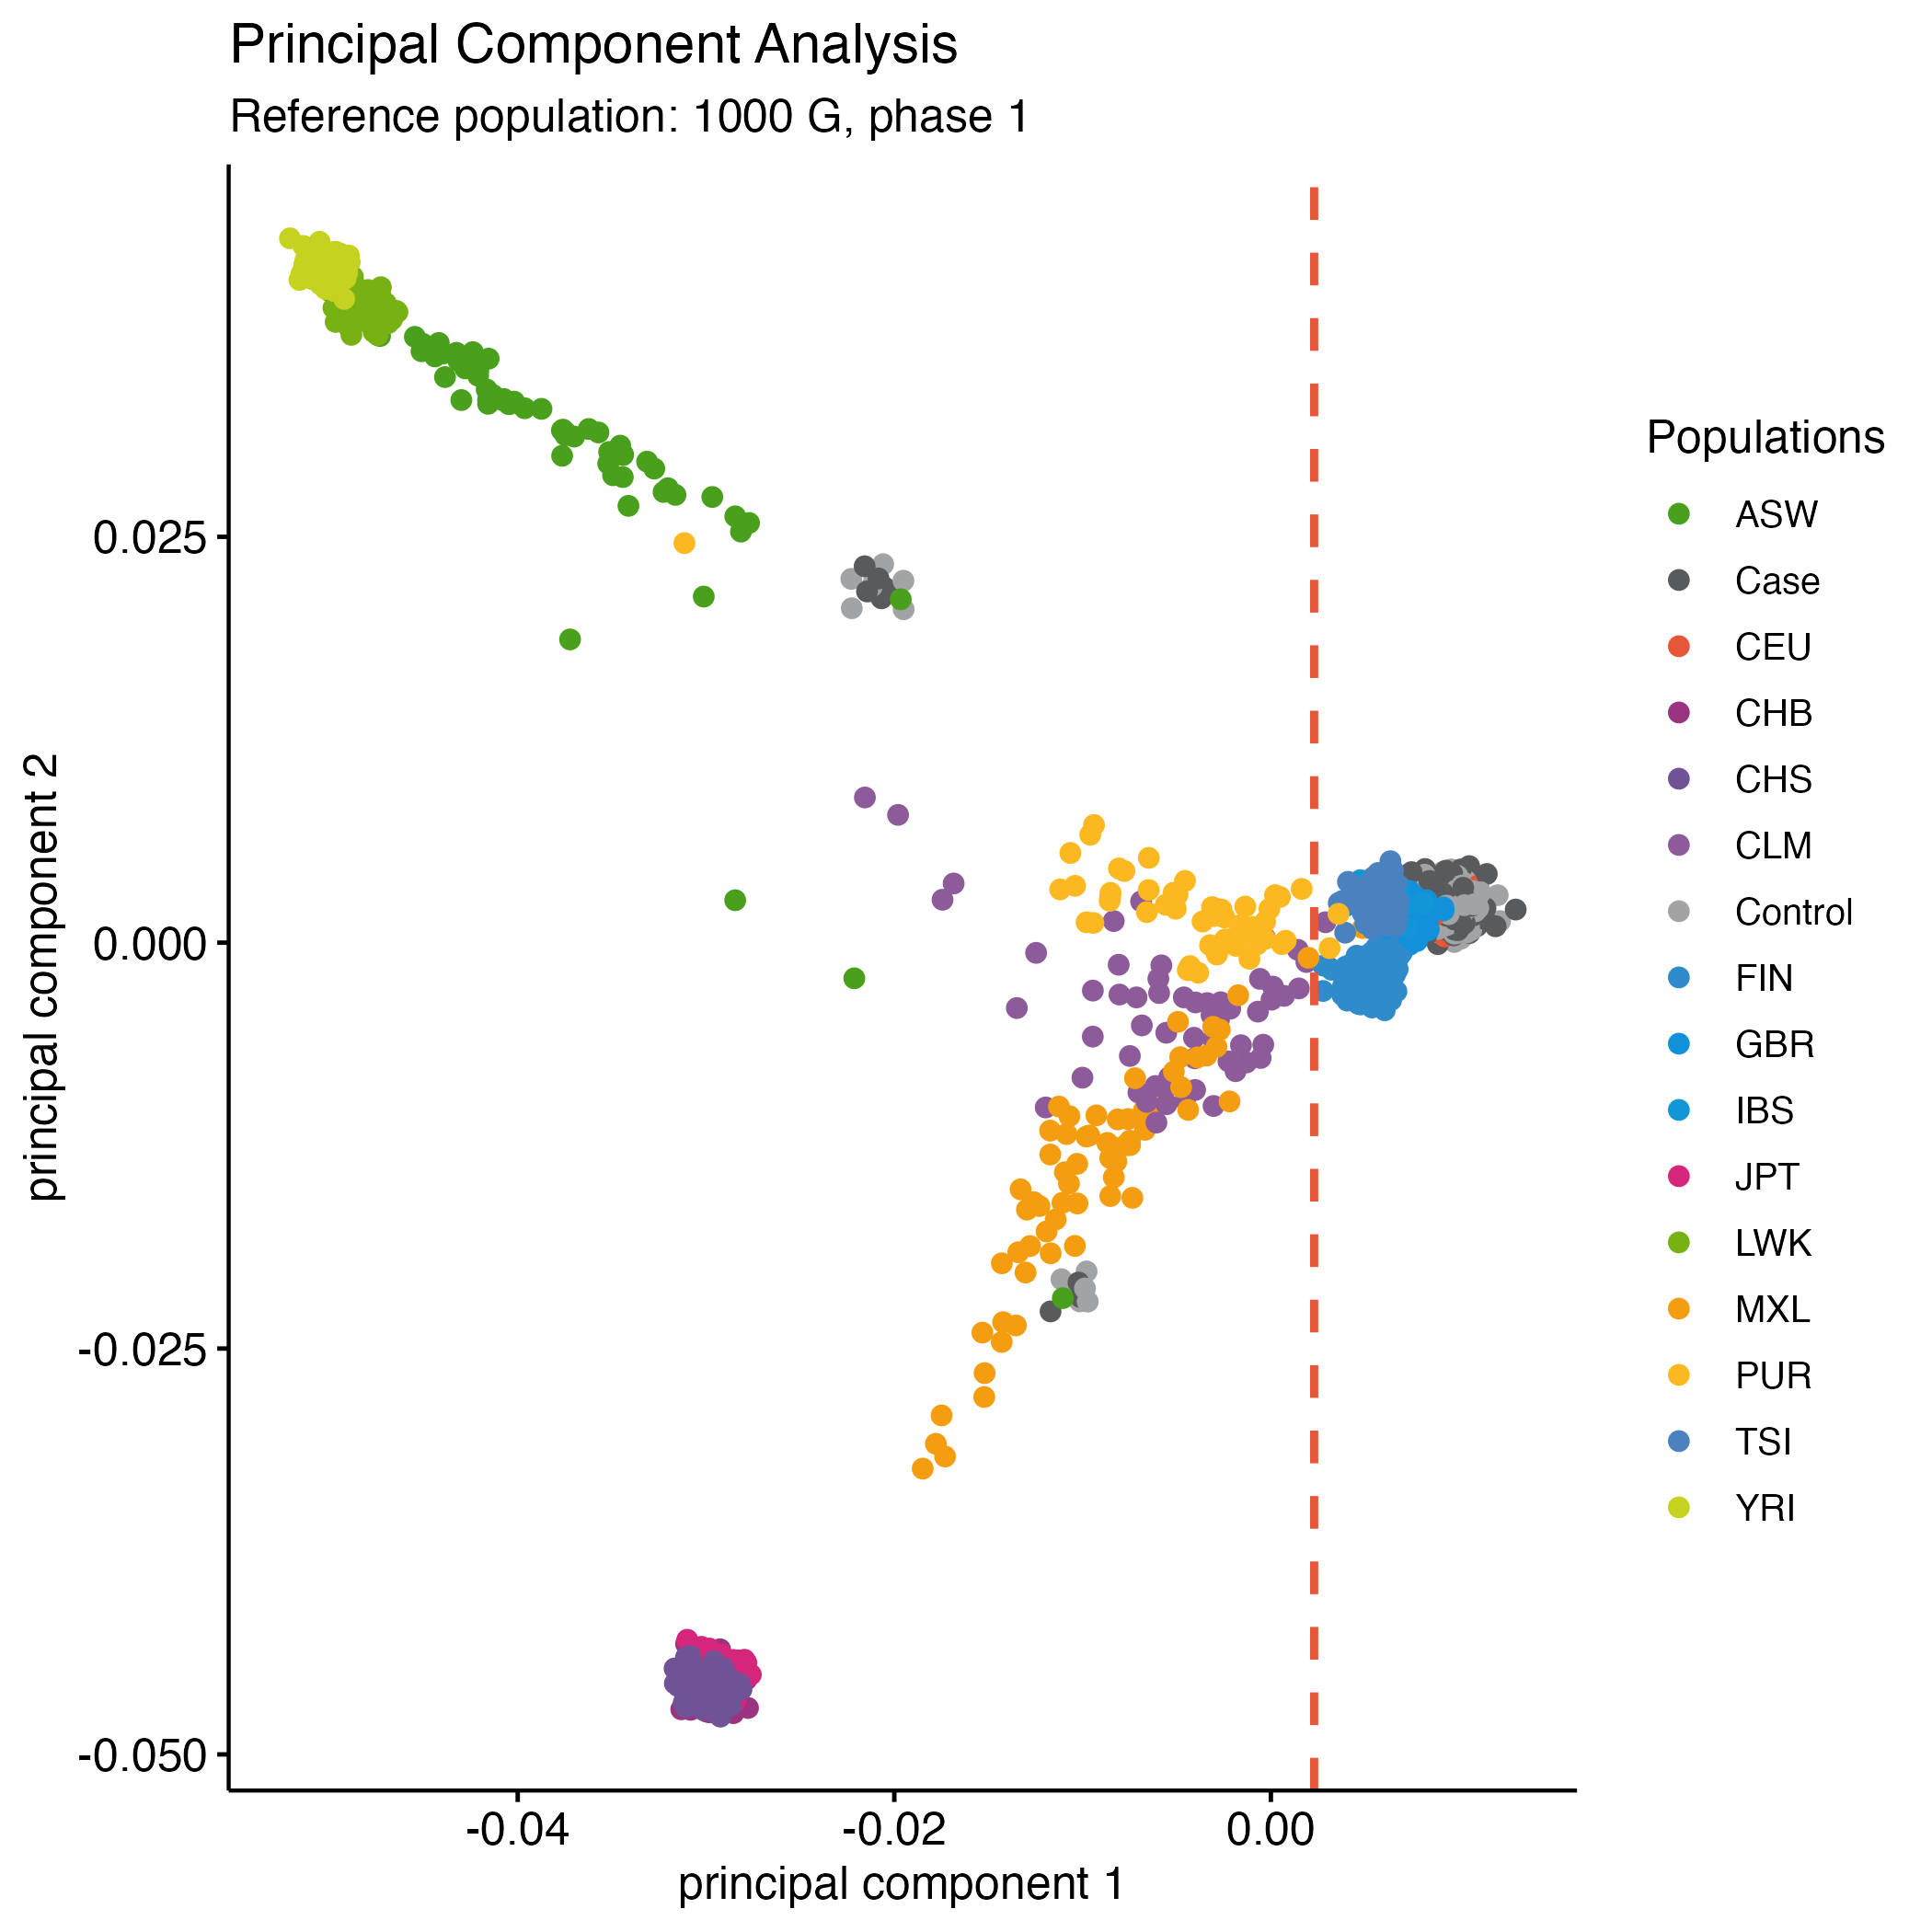
\includegraphics[width=0.85\linewidth]{img/_gwas_dummy/gwas-qc-pca-1000g} 

}

\caption{PCA - Your data vs. 1000g.}\label{fig:showpca1kg}
\end{figure}

\hypertarget{removing-samples}{%
\section{Removing samples}\label{removing-samples}}

Finally! We have a list of samples of poor quality or divergent ancestry, and duplicated or related samples. We should remove these. Let's collect all IDs from our \passthrough{\lstinline!fail-*!}-files into a single file.

\begin{lstlisting}
cat dummy_project/fail-* | sort -k1 | uniq > dummy_project/fail-qc-inds.txt
\end{lstlisting}

This new file should now contain a list of unique individuals failing the previous QC steps which we want to remove.

\begin{lstlisting}
plink --bfile dummy_project/rawdata --remove dummy_project/fail-qc-inds.txt --make-bed --out dummy_project/clean_inds_data
\end{lstlisting}

\begin{quote}
Question: How many variants and samples are left? How many cases and how many controls did you loose?
\end{quote}

\hypertarget{the-next-step}{%
\section{The next step}\label{the-next-step}}

Now that you filtered samples, we should turn our attention to step 2 of the QC for GWAS: identify SNPs of poor quality in Chapter @ref(gwas\_basics\_snp\_qc).

\hypertarget{gwas_basics_snp_qc}{%
\chapter{Per-SNP QC}\label{gwas_basics_snp_qc}}

Now that we removed samples, we can focus on low-quality variants.

\hypertarget{snp-call-rates}{%
\section{SNP call rates}\label{snp-call-rates}}

We start by calculating the missing genotype rate for each SNP, in other words the per-SNP call rate.

\begin{lstlisting}
plink --bfile dummy_project/clean_inds_data --missing --out dummy_project/clean_inds_data
\end{lstlisting}

Let's visualize the results to identify a threshold for extreme genotype failure rate. We chose a callrate threshold of 3\%, but it's arbitrary and depending on the dataset, the data (visualization), and the number of samples (Figure \ref{fig:showsnpcallrate}).

\begin{figure}[H]

{\centering 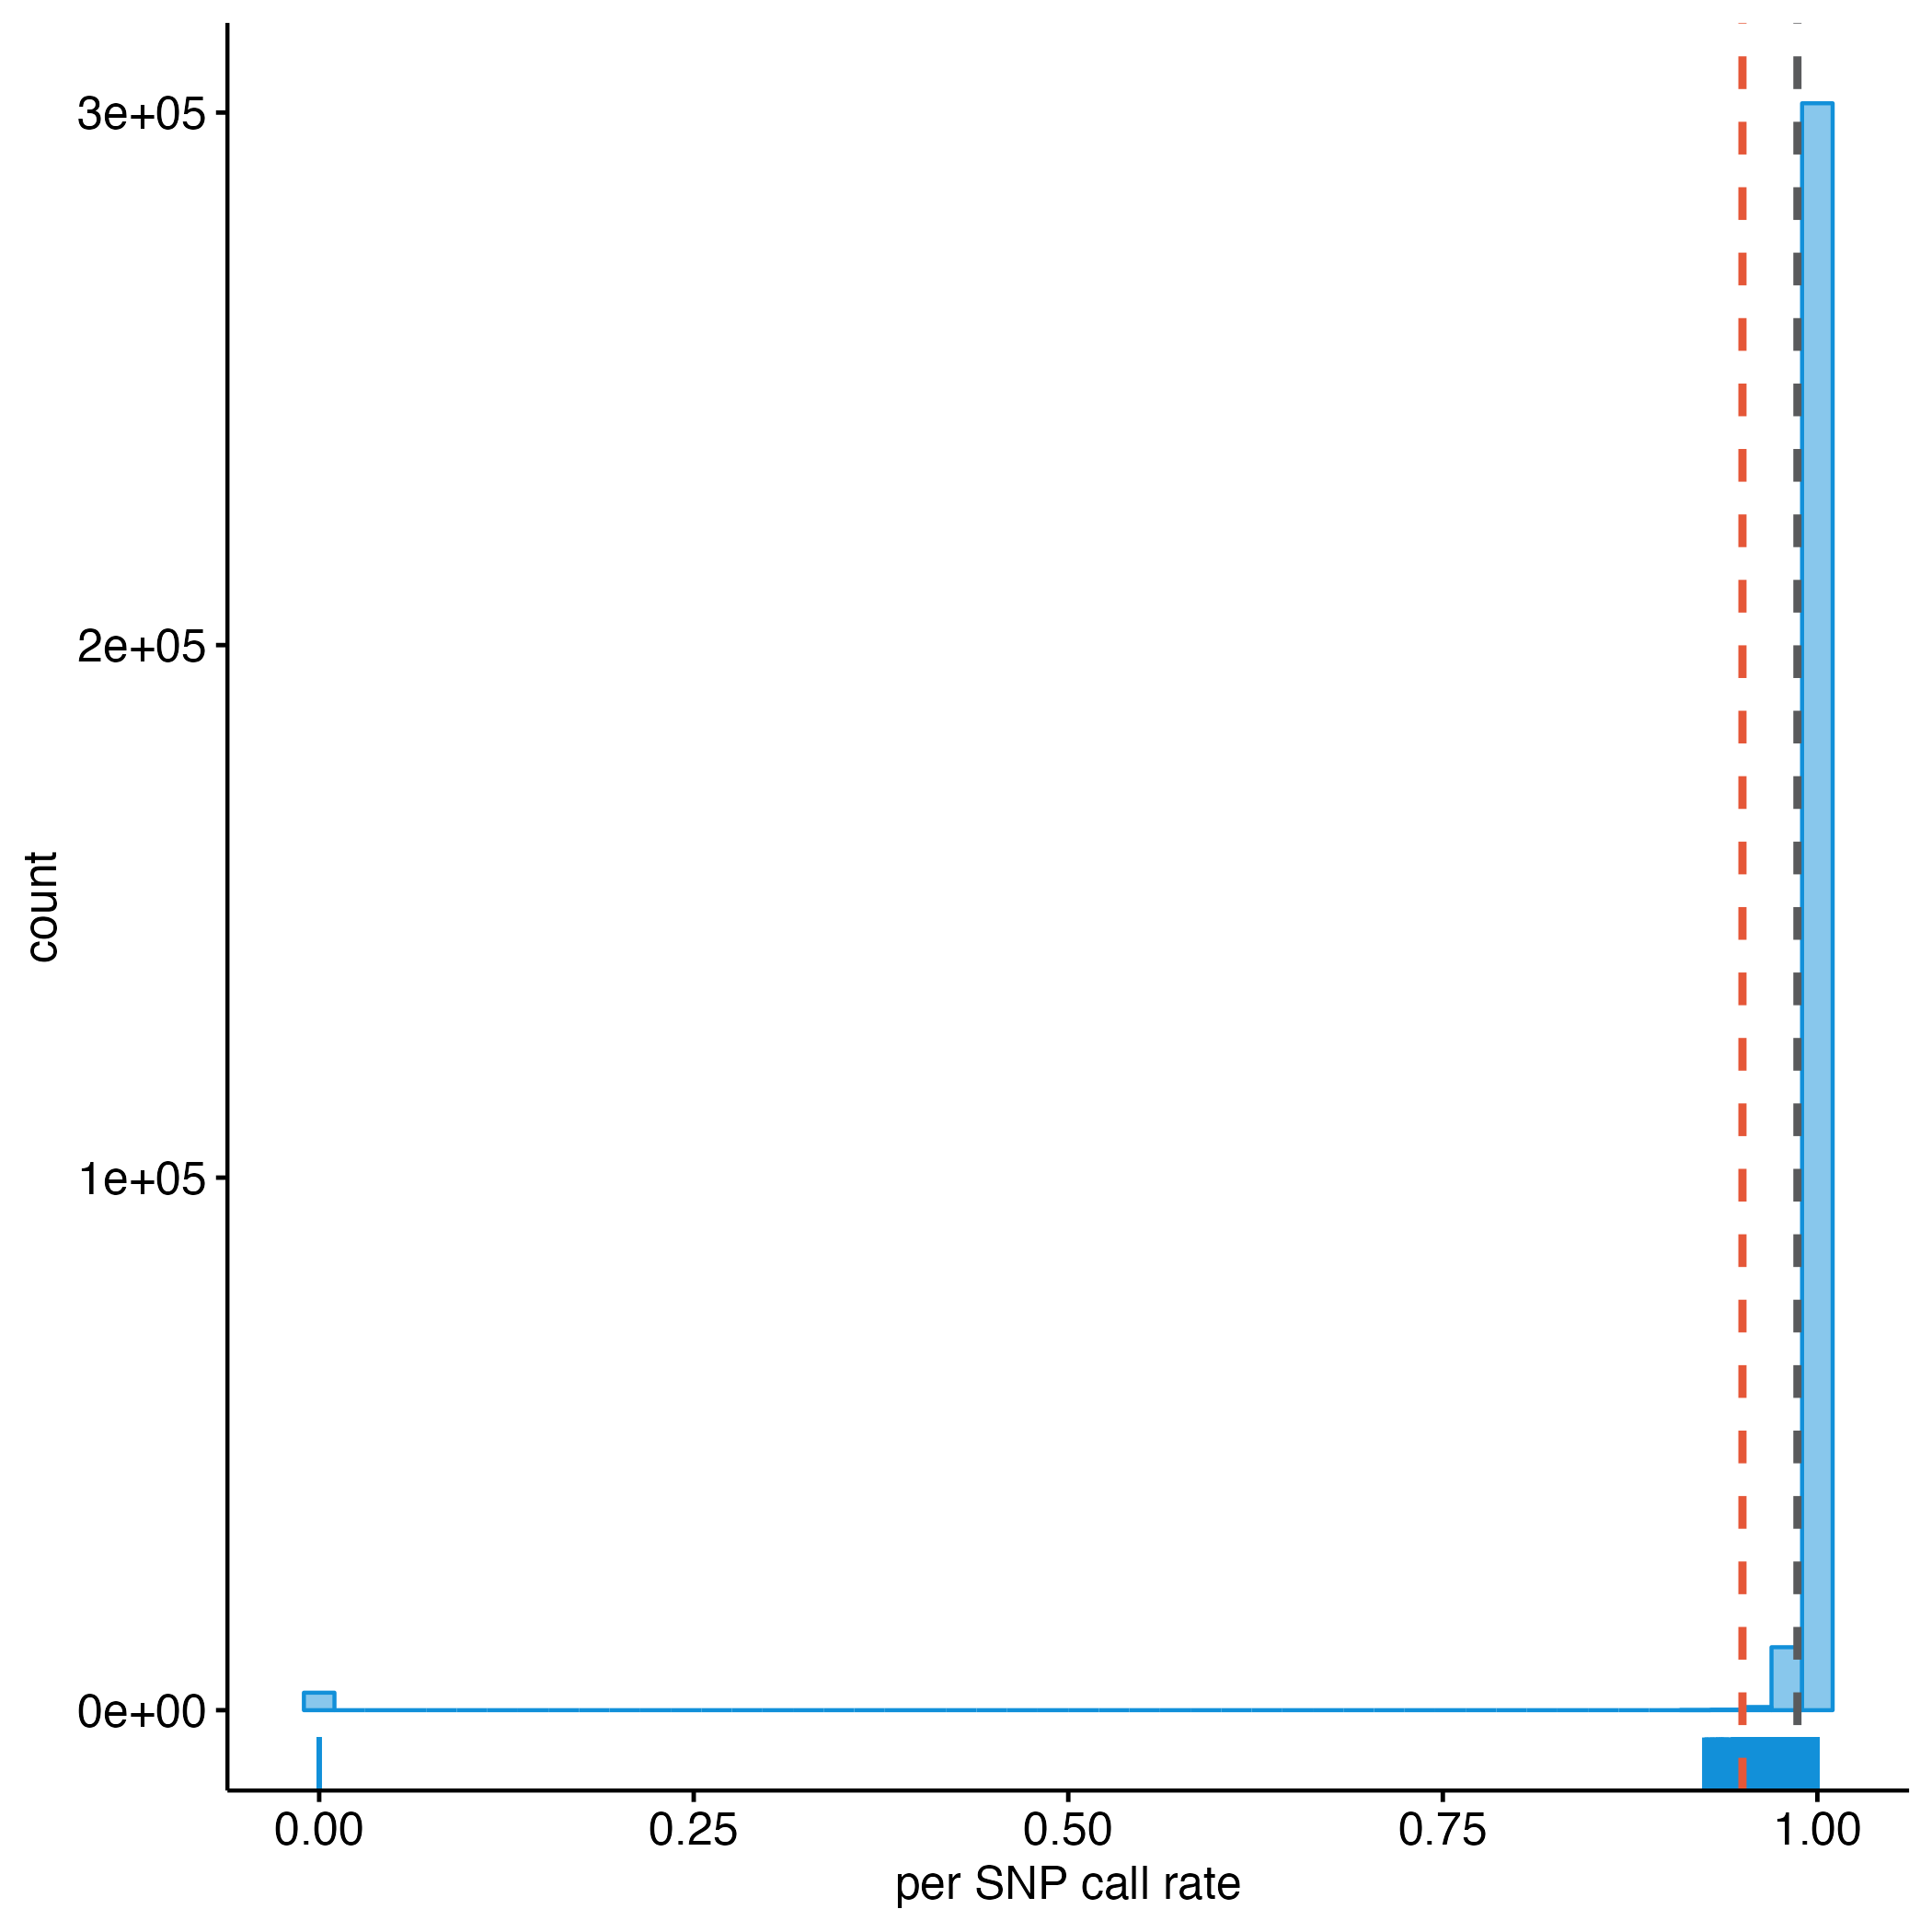
\includegraphics[width=0.85\linewidth]{img/_gwas_dummy/show-snp-callrate} 

}

\caption{Per SNP call rate.}\label{fig:showsnpcallrate}
\end{figure}

\hypertarget{differential-snp-call-rates}{%
\section{Differential SNP call rates}\label{differential-snp-call-rates}}

There could also be differences in genotype call rates between cases and controls. It is very important to check for this because these differences could lead to spurious associations. We can test all markers for differences in call rate between cases and controls, or based on other criteria.

\begin{lstlisting}
plink --bfile dummy_project/clean_inds_data --test-missing --out dummy_project/clean_inds_data
\end{lstlisting}

Let's collect all the SNPs with a significantly different (P \textless{} 0.00001) missing data rate between cases and controls.

\begin{lstlisting}
cat dummy_project/clean_inds_data.missing | awk '$5 < 0.00001' | awk '{ print $2 }' > dummy_project/fail-diffmiss-qc.txt
\end{lstlisting}

\hypertarget{allele-frequencies}{%
\section{Allele frequencies}\label{allele-frequencies}}

We should also get an idea on what the allele frequencies are in our dataset. Low frequent SNPs should probably be excluded, as these are uninformative when monomorphic (allele frequency = 0), or they may lead to spurious associations.

\begin{lstlisting}
plink --bfile dummy_project/clean_inds_data --freq --out dummy_project/clean_inds_data
\end{lstlisting}

Let's also plot these data. You can view the result below, and try it yourself (Figure \ref{fig:showfreq}).

\begin{figure}[H]

{\centering 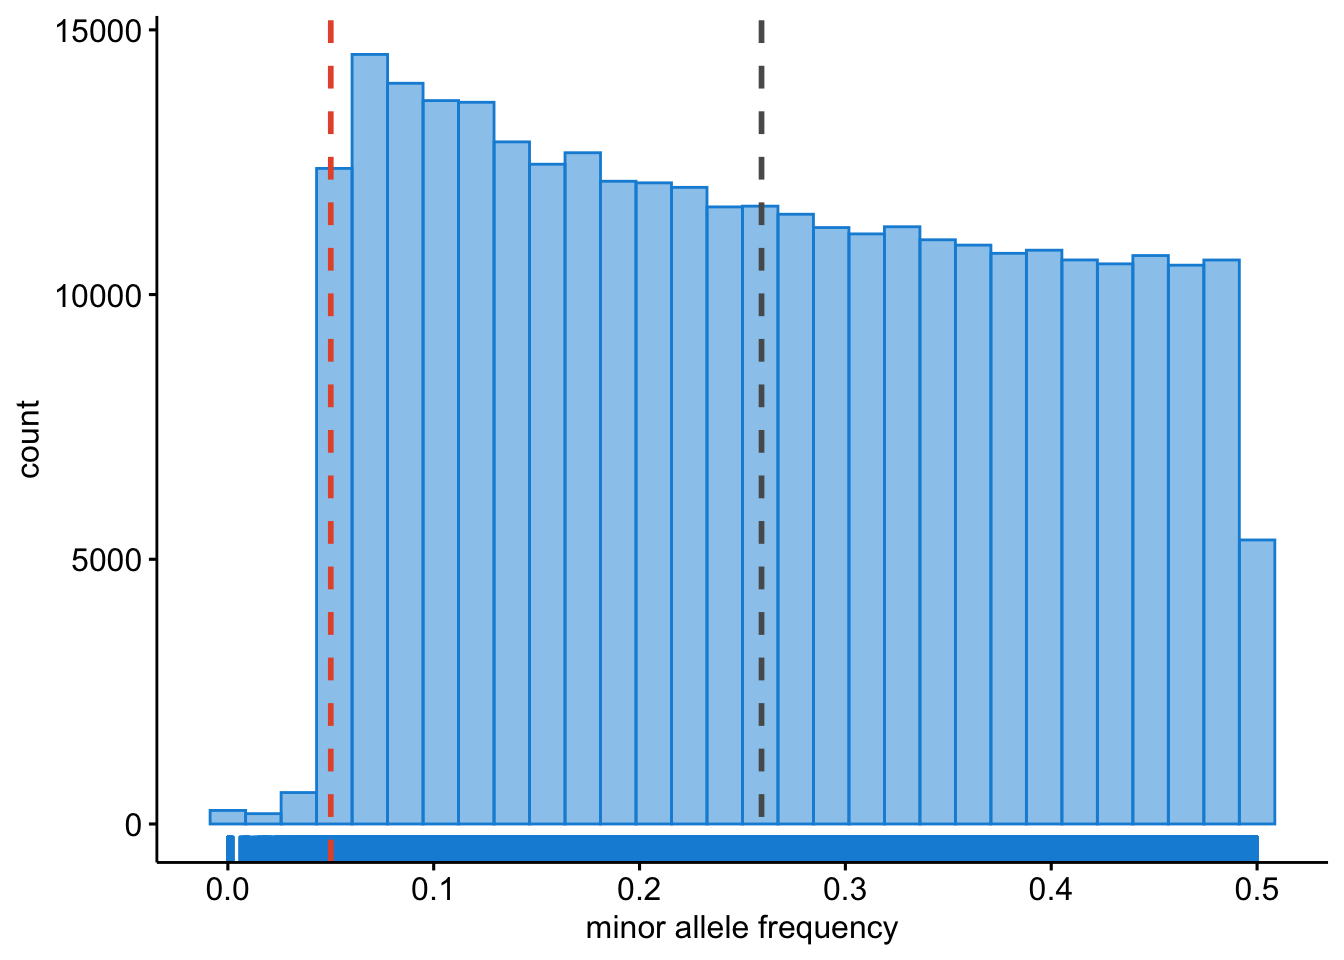
\includegraphics[width=0.85\linewidth]{img/_gwas_dummy/show-freq} 

}

\caption{Minor allele frequency.}\label{fig:showfreq}
\end{figure}

\hypertarget{a-note-on-allele-coding}{%
\subsection{A note on allele coding}\label{a-note-on-allele-coding}}

Oh, one more thing about alleles.

\passthrough{\lstinline!PLINK!} codes alleles as follows:

A1 = minor allele, the least frequent allele
A2 = major allele, the most frequent allele

And when you use \passthrough{\lstinline!PLINK!} the flag \passthrough{\lstinline!--freq!} or \passthrough{\lstinline!--maf!} is always relative to the A1-allele, as is the odds ratio (OR) or effect size (beta).

However, \passthrough{\lstinline!SNPTEST!} makes use of the so-called OXFORD-format, this codes alleles as follows:

A = the `other' allele
B = the `coded' allele

When you use \passthrough{\lstinline!SNPTEST!} it will report the allele frequency as \passthrough{\lstinline!CAF!}, in other words the \emph{coded allele frequency}, and the effect size (beta) is always relative to the B-allele. This means, \passthrough{\lstinline!CAF!} \emph{could} be the \passthrough{\lstinline!MAF!}, or \emph{minor allele frequency}, but this is \textbf{not} a given.

In other words, always make sure what the allele-coding of a given program, be it \passthrough{\lstinline!PLINK!}, \passthrough{\lstinline!SNPTEST!}, \passthrough{\lstinline!GCTA!}, \emph{et cetera}, is! I cannot stress this enough. Ask yourself: `what is the allele frequency referring to?', `the effect size is relative to\ldots?'.

Right, let's continue.

\hypertarget{hardy-weinberg-equilibrium}{%
\section{Hardy-Weinberg Equilibrium}\label{hardy-weinberg-equilibrium}}

Because we are performing a case-control genome-wide association study, we probably expect some differences in Hardy-Weinberg Equilibrium (HWE), but extreme deviations are probably indicative of genotyping errors.

\begin{lstlisting}
plink --bfile dummy_project/clean_inds_data --hardy --out dummy_project/clean_inds_data
\end{lstlisting}

Let's also plot these data. You can view the result below, and type over the code to do it yourself.

\begin{figure}[H]

{\centering 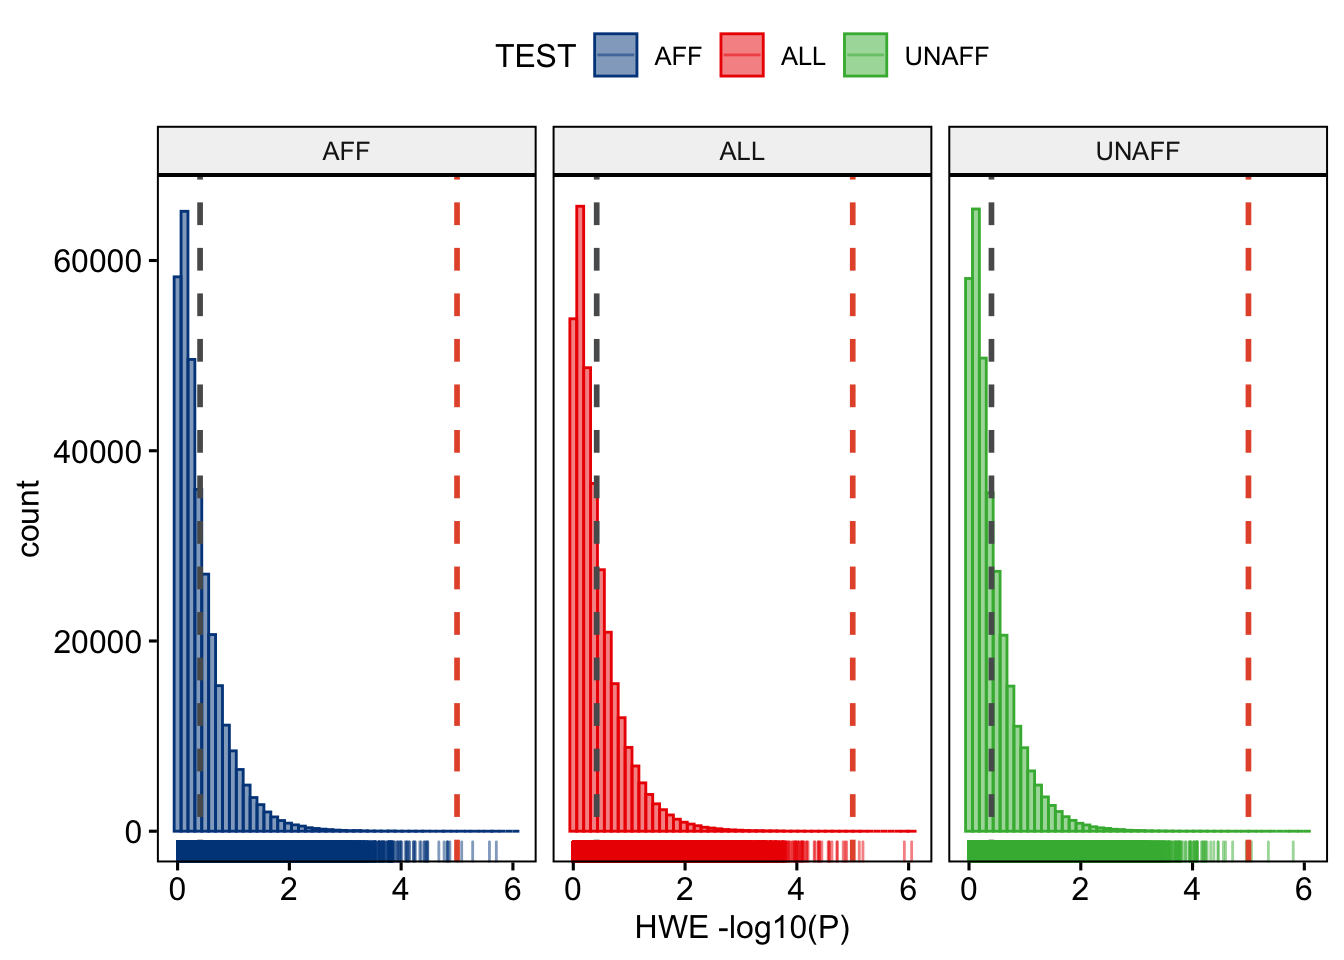
\includegraphics[width=0.85\linewidth]{img/_gwas_dummy/show-hwe} 

}

\caption{Hardy-Weinberg Equilibrium p-values per stratum.}\label{fig:showhwe}
\end{figure}

\hypertarget{final-snp-qc}{%
\section{Final SNP QC}\label{final-snp-qc}}

We are ready to perform the final QC. After inspecting the graphs we will filter on a MAF \textless{} 0.01, call rate \textless{} 0.05, and HWE \textless{} 0.00001 (Figure \ref{fig:showhwe}), in addition those SNPs that failed the differential call rate test will be removed.

\begin{lstlisting}
plink --bfile dummy_project/clean_inds_data --exclude dummy_project/fail-diffmiss-qc.txt --maf 0.01 --geno 0.05 --hwe 0.00001 --make-bed --out dummy_project/cleandata
\end{lstlisting}

\hypertarget{a-milestone}{%
\section{A Milestone}\label{a-milestone}}

Congratulations. You reached a very important milestone. Now that you filtered samples and SNPs, we can finally start the association analyses in Chapter @ref(gwas\_testing).

\hypertarget{gwas_testing}{%
\chapter{Genome-Wide Association Study}\label{gwas_testing}}

Now that you have learned how to perform QC, you can easily run a GWAS and execute some downstream visualization and analyses. Let's do this with a dummy dataset.

\hypertarget{exploring-the-data}{%
\section{Exploring the data}\label{exploring-the-data}}

Even though someone says that the QC was done, it is still wise and good practice to run some of the commands above to get a `feeling' about the data. So let's do this.

\begin{lstlisting}
plink --bfile gwas/gwa --freq --out dummy_project/gwa
\end{lstlisting}

\begin{lstlisting}
plink --bfile gwas/gwa --missing --out dummy_project/gwa
\end{lstlisting}

\begin{lstlisting}
plink --bfile gwas/gwa --hardy --out dummy_project/gwa
\end{lstlisting}

Let's visualize the results. First we should load in all the results.

\begin{quote}
Question: Load the data using R. {[}Hint: use and adapt the examples from the previous chapters.{]}
\end{quote}

We can plot the per-stratum HWE p-values.

\begin{quote}
Question: Plot the per-stratum HWE p-values using R. {[}Hint: use and adapt the examples from the previous chapters.{]}
\end{quote}

\begin{figure}[H]

{\centering 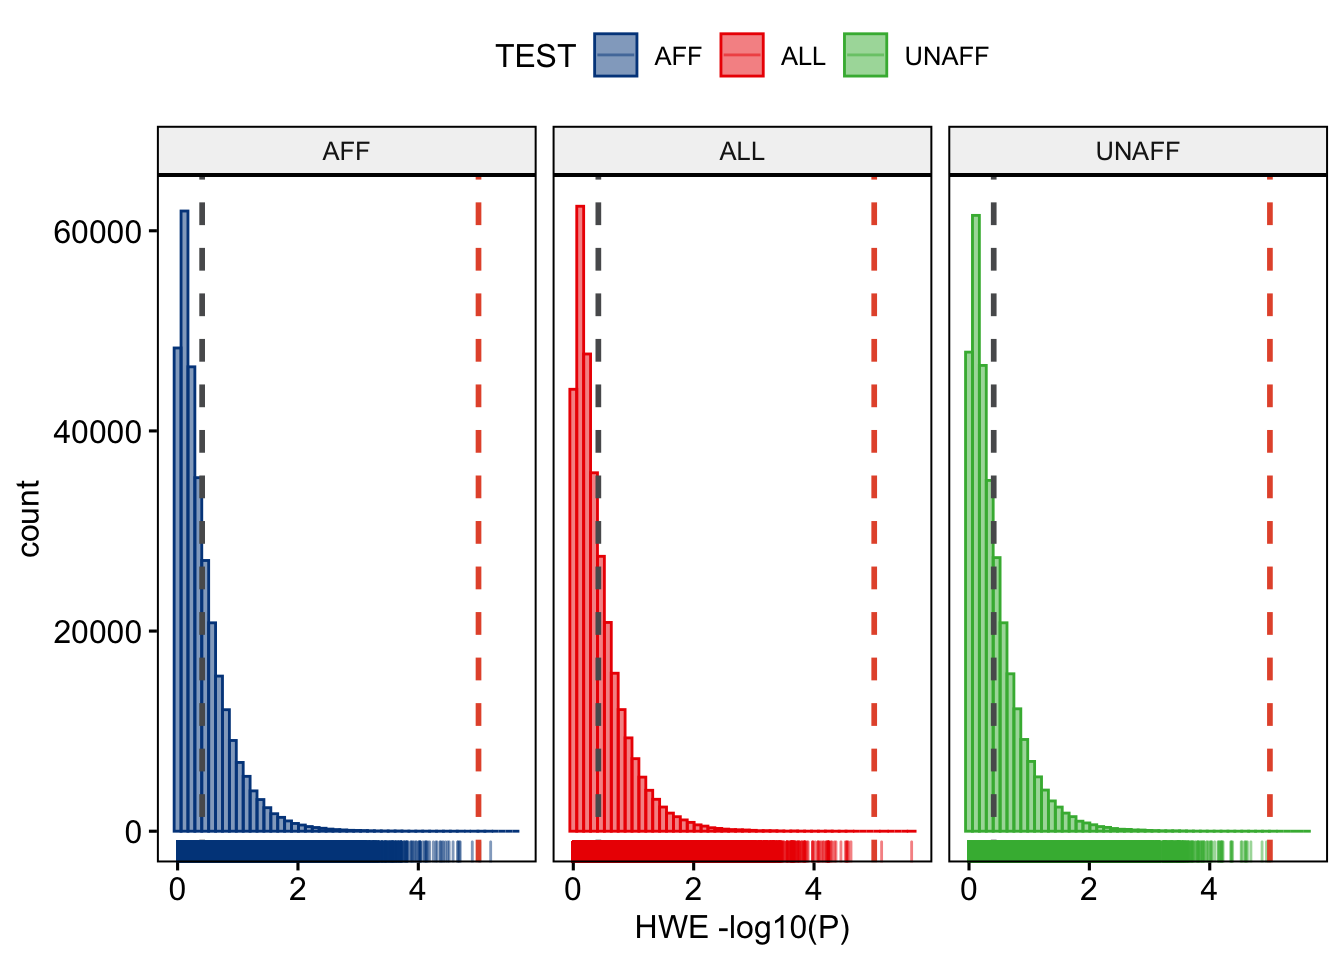
\includegraphics[width=0.85\linewidth]{img/_gwas_dummy/show-hwe-gwas} 

}

\caption{Per stratum HWE p-values.}\label{fig:unnamed-chunk-2}
\end{figure}

We will want to see what the distribution of allele frequencies looks like.

\begin{quote}
Question: Plot the allele frequencies using R. {[}Hint: use and adapt the examples from the previous chapters.{]}
\end{quote}

\begin{figure}[H]

{\centering 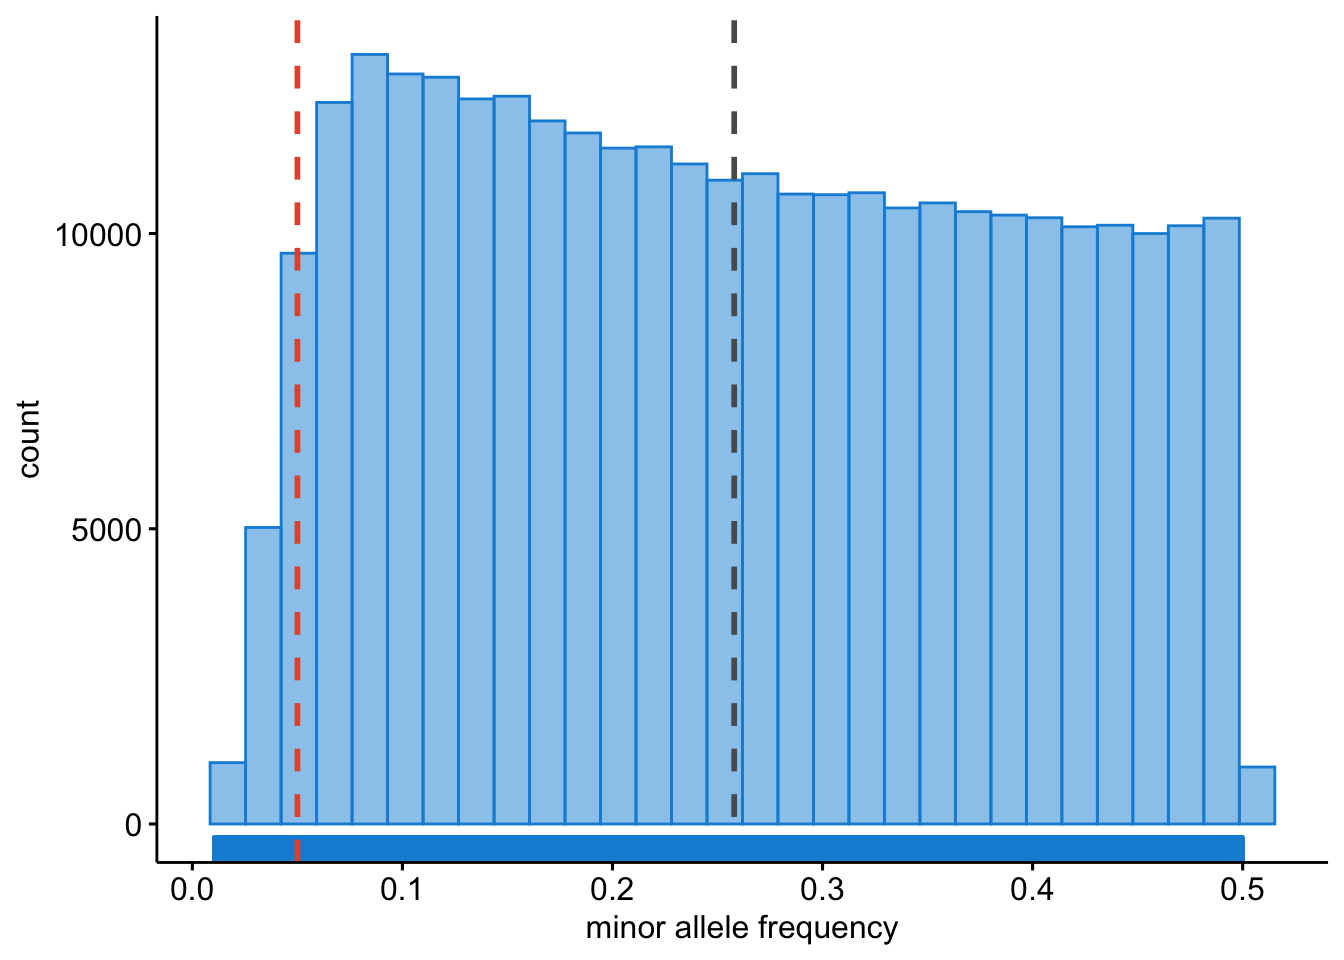
\includegraphics[width=0.85\linewidth]{img/_gwas_dummy/show-freq-gwas} 

}

\caption{Minor allele frequencies.}\label{fig:unnamed-chunk-3}
\end{figure}

We will want to identify samples that have poor call rates.

\begin{quote}
Question: Plot the per-sample call rates using R. {[}Hint: use and adapt the examples from the previous chapters.{]}
\end{quote}

\begin{figure}[H]

{\centering 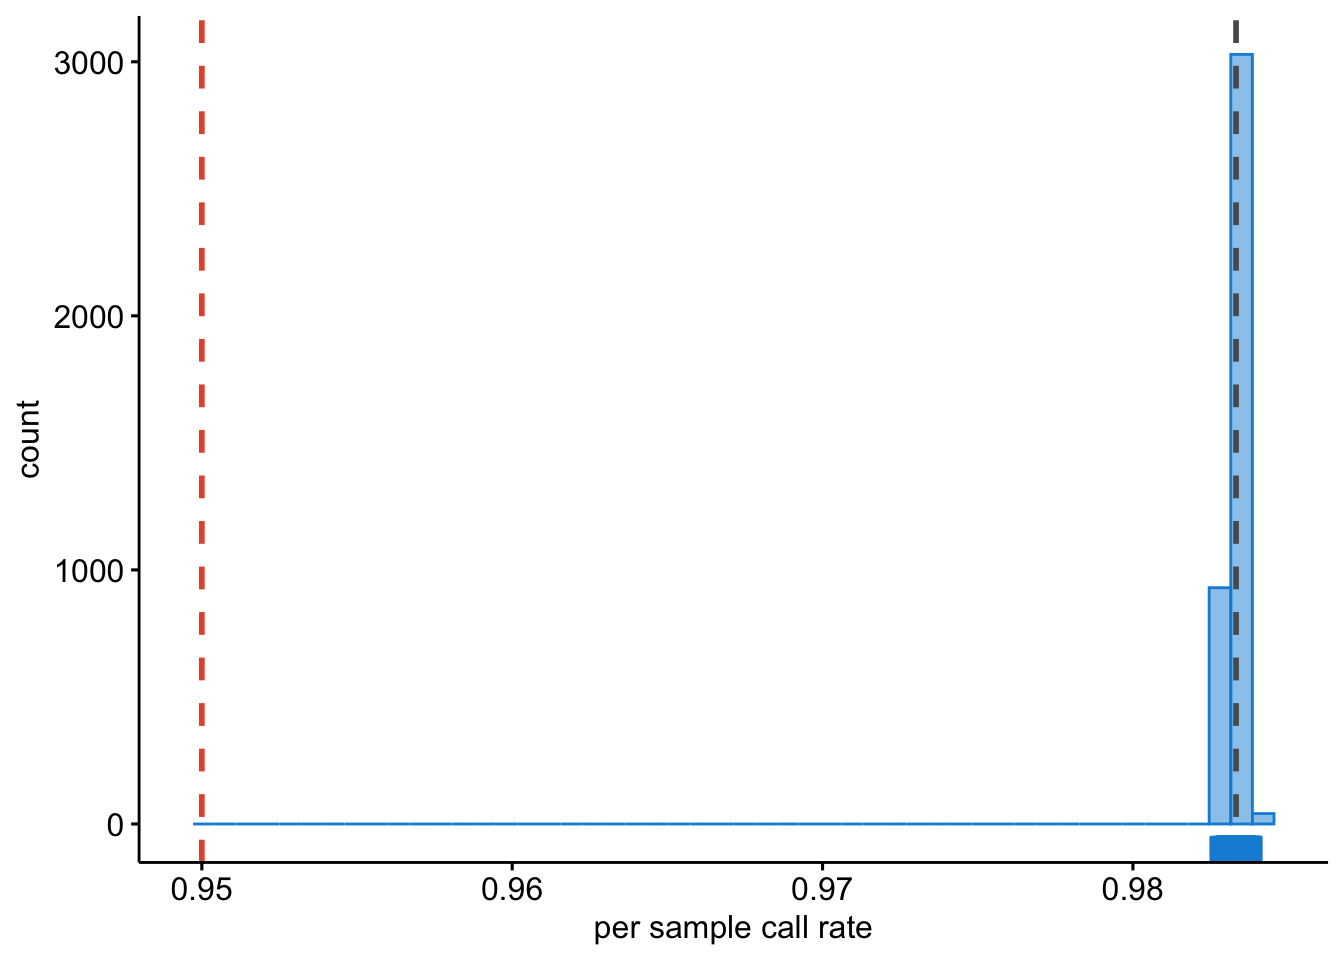
\includegraphics[width=0.85\linewidth]{img/_gwas_dummy/show-sample-callrate-gwas} 

}

\caption{Per sample call rates.}\label{fig:unnamed-chunk-4}
\end{figure}

We also need to know what the per SNP call rates are.

\begin{quote}
Question: Plot the per-SNP call rates using R. {[}Hint: use and adapt the examples from the previous chapters.{]}
\end{quote}

\begin{figure}[H]

{\centering 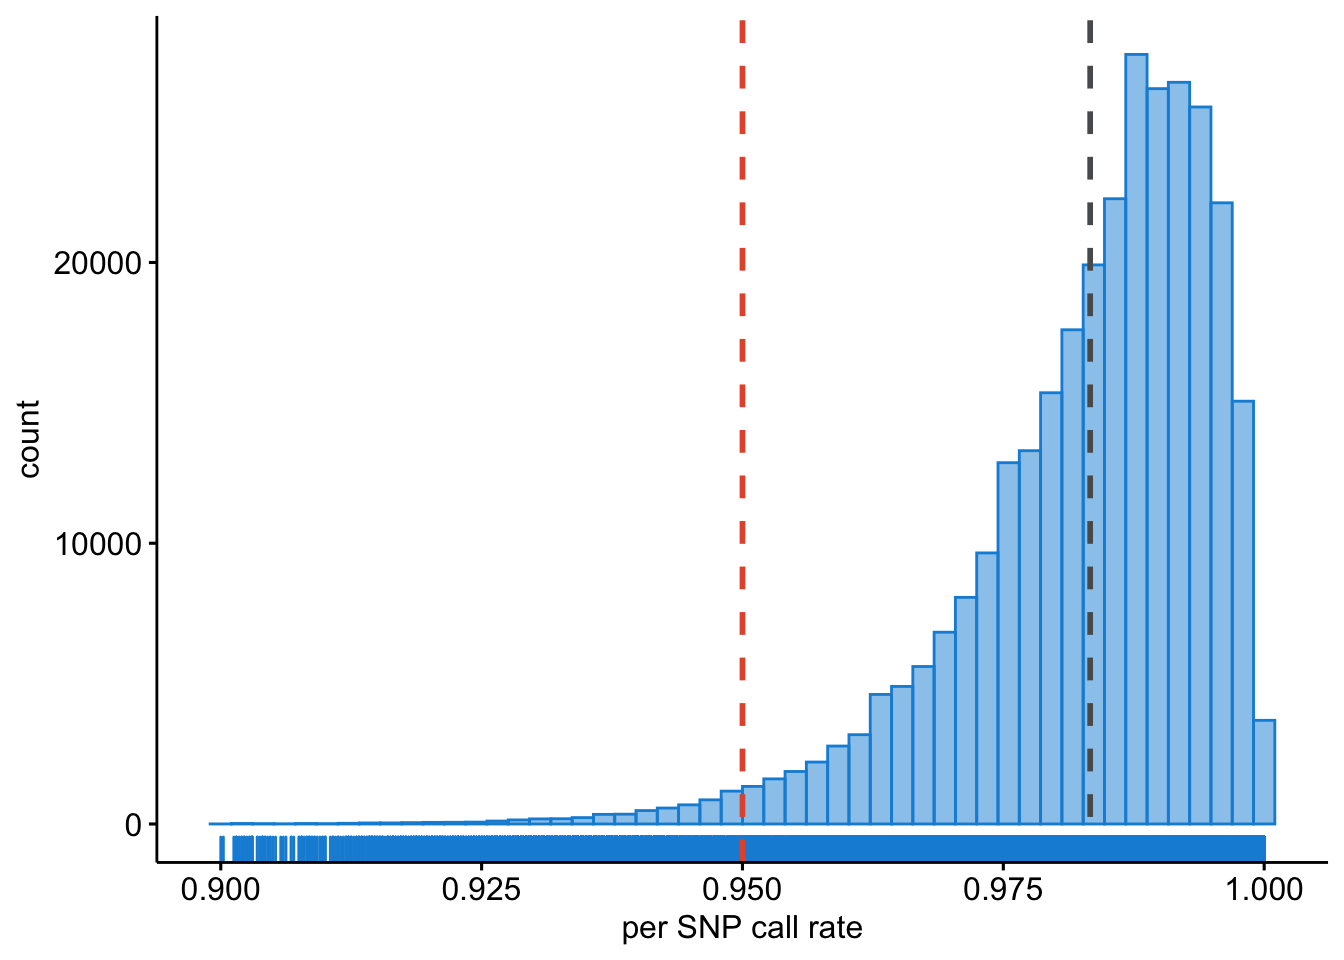
\includegraphics[width=0.85\linewidth]{img/_gwas_dummy/show-snp-callrate-gwas} 

}

\caption{Per SNP call rates.}\label{fig:unnamed-chunk-5}
\end{figure}

\hypertarget{genetic-models}{%
\section{Genetic models}\label{genetic-models}}

A simple chi-square test of association can be done.

\begin{lstlisting}
plink --bfile gwas/gwa --model --out gwas/data
\end{lstlisting}

\emph{Genotypic}, \emph{dominant} and \emph{recessive} tests will not be conducted if any one of the cells in the table of case-control by genotype counts contains less than five observations. This is because the chi-square approximation may not be reliable when cell counts are small. For SNPs with MAFs \textless{} 5\%, a sample of more than 2,000 cases and controls would be required to meet this threshold and more than 50,000 would be required for SNPs with MAF \textless{} 1\%.

You can change this default behaviour by adding the flag \passthrough{\lstinline!--cell!}, \emph{e.g.}, we could lower the threshold to 3.

\begin{lstlisting}
plink --bfile gwas/gwa --model --cell 3 --out gwas/data
\end{lstlisting}

Let's review the contents of the results.

It contains 1,530,510 rows, one for each SNP, and each type of test (\emph{genotypic}, \emph{trend}, \emph{allelic}, \emph{dominant}, and \emph{recessive}) and the following columns:

\begin{itemize}
\tightlist
\item
  chromosome {[}\passthrough{\lstinline!CHR!}{]},
\item
  the SNP identifier {[}\passthrough{\lstinline!SNP!}{]},
\item
  the minor allele {[}\passthrough{\lstinline!A1!}{]} (remember, \passthrough{\lstinline!PLINK!} always codes the A1-allele as the minor allele!),
\item
  the major allele {[}\passthrough{\lstinline!A2!}{]},
\item
  the test performed {[}\passthrough{\lstinline!TEST!}{]}:

  \begin{itemize}
  \tightlist
  \item
    \passthrough{\lstinline!GENO!} (genotypic association);
  \item
    \passthrough{\lstinline!TREND!} (Cochran-Armitage trend);
  \item
    \passthrough{\lstinline!ALLELIC!} (allelic as- sociation);
  \item
    \passthrough{\lstinline!DOM!} (dominant model); and
  \item
    \passthrough{\lstinline!REC!} (recessive model){]},
  \end{itemize}
\item
  the cell frequency counts for cases {[}\passthrough{\lstinline!AFF!}{]},
\item
  the cell frequency counts for controls {[}\passthrough{\lstinline!UNAFF!}{]},
\item
  the chi-square test statistic {[}\passthrough{\lstinline!CHISQ!}{]},
\item
  the degrees of freedom for the test {[}\passthrough{\lstinline!DF!}{]},
\item
  and the asymptotic P value {[}\passthrough{\lstinline!P!}{]} of association.
\end{itemize}

\begin{quote}
Question: Do you know which model, \emph{i.e.} \passthrough{\lstinline!TEST!} is most commonly used and reported? And why is that, do think?
\end{quote}

\hypertarget{logistic-regression}{%
\section{Logistic regression}\label{logistic-regression}}

We can also perform a test of association using logistic regression. In this case we might want to correct for covariates/confounding factors, for example age, sex, ancestral background, i.e.~principal components, and other study specific covariates (e.g.~hospital of inclusion, genotyping centre etc.). In that case each of these P values is adjusted for the effect of the covariates.

When running a regression analysis, be it linear or logistic, PLINK assumes a multiplicative model. By default, when at least one male and one female is present, sex (male = 1, female = 0) is automatically added as a covariate on X chromosome SNPs, and nowhere else. The \passthrough{\lstinline!sex!} flag causes it to be added everywhere, while \passthrough{\lstinline!no-x-sex!} excludes it.

\begin{lstlisting}
plink --bfile gwas/gwa --logistic sex --covar gwas/gwa.covar --out gwas/data
\end{lstlisting}

Let's examine the results.

\begin{lstlisting}
## [1] 918306      9
\end{lstlisting}

\begin{lstlisting}
##      CHR       SNP      BP     A1   TEST NMISS     OR
##    <int>    <char>   <int> <char> <char> <int>  <num>
## 1:     1 rs3934834  995669      T    ADD  3818 1.0290
## 2:     1 rs3934834  995669      T    AGE  3818 1.0020
## 3:     1 rs3934834  995669      T    SEX  3818 1.0120
## 4:     1 rs3737728 1011278      A    ADD  3982 1.0190
## 5:     1 rs3737728 1011278      A    AGE  3982 1.0020
## 6:     1 rs3737728 1011278      A    SEX  3982 1.0060
## 7:     1 rs6687776 1020428      T    ADD  3915 0.9692
## 8:     1 rs6687776 1020428      T    AGE  3915 1.0020
## 9:     1 rs6687776 1020428      T    SEX  3915 1.0150
##        STAT      P
##       <num>  <num>
## 1:  0.38120 0.7031
## 2:  1.11800 0.2635
## 3:  0.19090 0.8486
## 4:  0.38670 0.6990
## 5:  1.09800 0.2721
## 6:  0.09898 0.9212
## 7: -0.33330 0.7389
## 8:  1.04000 0.2984
## 9:  0.23690 0.8127
\end{lstlisting}

\begin{quote}
Question: How come there are more lines in this file than there are variants?
\end{quote}

If no model option is specified, the first row for each SNP corresponds to results for a multiplicative test of association. The C \textgreater= 0 subsequent rows for each SNP correspond to separate tests of significance for each of the C covariates included in the regression model. We can remove the covariate-specific lines from the main report by adding the \passthrough{\lstinline!hide-covar!} flag.

The columns in the association results are:

\begin{itemize}
\tightlist
\item
  the chromosome {[}\passthrough{\lstinline!CHR!}{]},
\item
  the SNP identifier {[}\passthrough{\lstinline!SNP!}{]},
\item
  the base-pair location {[}\passthrough{\lstinline!BP!}{]},
\item
  the minor allele {[}\passthrough{\lstinline!A1!}{]},
\item
  the test performed {[}\passthrough{\lstinline!TEST!}{]}: ADD (multiplicative model or genotypic model testing additivity),

  \begin{itemize}
  \tightlist
  \item
    \passthrough{\lstinline!GENO\_2DF!} (genotypic model),
  \item
    \passthrough{\lstinline!DOMDEV!} (genotypic model testing deviation from additivity),
  \item
    \passthrough{\lstinline!DOM!} (dominant model), or
  \item
    \passthrough{\lstinline!REC!} (recessive model){]},
  \end{itemize}
\item
  the number of missing individuals included {[}\passthrough{\lstinline!NMISS!}{]},
\item
  the \passthrough{\lstinline!OR!} relative to the A1, \emph{i.e.} minor allele,
\item
  the coefficient z-statistic {[}\passthrough{\lstinline!STAT!}{]}, and
\item
  the asymptotic P-value {[}\passthrough{\lstinline!P!}{]} of association.
\end{itemize}

We need to calculate the standard error and confidence interval from the z-statistic. We can modify the effect size (\passthrough{\lstinline!OR!}) to output the \emph{beta} by adding the \passthrough{\lstinline!beta!} flag.

\begin{quote}
Question: Can you write down the mathematical relation between \emph{beta} and \emph{OR}?
\end{quote}

\hypertarget{lets-get-visual}{%
\section{Let's get visual}\label{lets-get-visual}}

Looking at numbers is important, but it won't give you a perfect overview. We should turn to visualizing our results in Chapter \ref{gwas-visuals}.

\hypertarget{gwas-visuals}{%
\chapter{GWAS visualisation}\label{gwas-visuals}}

Data visualization is key, not only for presentation but also to inspect the results.

\hypertarget{qq-plots}{%
\subsection{QQ plots}\label{qq-plots}}

We should create \emph{quantile-quantile (QQ) plots} to compare the observed association test statistics with their expected values under the null hypothesis of no association and so assess the number, magnitude and quality of true associations.

First, we will add the standard error, call rate, A2, and allele frequencies.

\begin{lstlisting}
## Key: <SNP>
##           SNP   CHR        BP     A1 NMISS     OR
##        <char> <int>     <int> <char> <int>  <num>
## 1: rs10000010     4  21227772      C  3996 1.0420
## 2: rs10000023     4  95952929      T  3957 0.9902
## 3: rs10000030     4 103593179      A  3991 0.9779
## 4:  rs1000007     2 237416793      C  4000 1.0180
## 5: rs10000092     4  21504615      C  3963 0.9240
## 6: rs10000121     4 157793485      G  3919 0.9665
##       STAT       P     A2    MAF NCHROBS callrate
##      <num>   <num> <char>  <num>   <int>    <num>
## 1:  0.9010 0.36760      T 0.4258    7992  0.99900
## 2: -0.2160 0.82900      G 0.4841    7914  0.98925
## 3: -0.3696 0.71170      G 0.1616    7982  0.99775
## 4:  0.3649 0.71520      T 0.3122    8000  1.00000
## 5: -1.6770 0.09354      T 0.3430    7926  0.99075
## 6: -0.7525 0.45170      A 0.4532    7838  0.97975
\end{lstlisting}

\begin{lstlisting}
## [1] 306102     14
\end{lstlisting}

\begin{lstlisting}
## # A tibble: 6 x 14
##   SNP        CHR     BP A1    A2      MAF callrate NMISS
##   <chr>    <int>  <int> <chr> <chr> <dbl>    <dbl> <int>
## 1 rs10000~     4 2.12e7 C     T     0.426    0.999  3996
## 2 rs10000~     4 9.60e7 T     G     0.484    0.989  3957
## 3 rs10000~     4 1.04e8 A     G     0.162    0.998  3991
## 4 rs10000~     2 2.37e8 C     T     0.312    1      4000
## 5 rs10000~     4 2.15e7 C     T     0.343    0.991  3963
## 6 rs10000~     4 1.58e8 G     A     0.453    0.980  3919
## # i 6 more variables: NCHROBS <int>, BETA <dbl>,
## #   SE <dbl>, OR <dbl>, STAT <dbl>, P <dbl>
\end{lstlisting}

Let's list the number of SNPs per chromosome. This gives a pretty good idea about the per-chromosome coverage. And it's a sanity check: did the whole analysis run properly (we expect 22 chromosomes)?

\begin{quote}
Question: Why do the number of variants per chrosome (approximately) correlate with the chromosome number?
\end{quote}

\begin{quote}
Question: Where are the data for chromosome X, Y and MT?
\end{quote}

Let's plot the QQ plot to diagnose our GWAS.

\begin{figure}[H]

{\centering 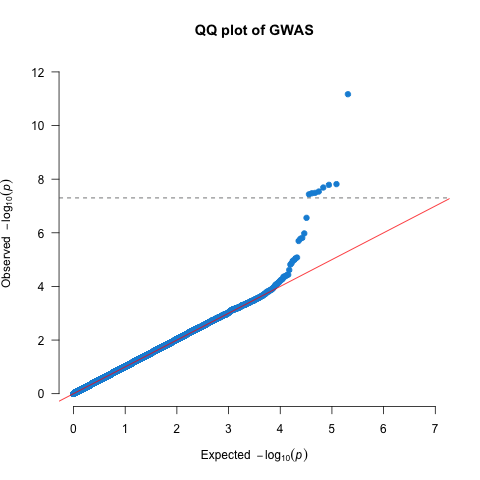
\includegraphics[width=0.85\linewidth]{img/_gwas_dummy/show-qq} 

}

\caption{A QQ plot.}\label{fig:show-qq}
\end{figure}

\hypertarget{manhattan-plots}{%
\section{Manhattan plots}\label{manhattan-plots}}

We also need to create a \emph{Manhattan plot} to display the association test P-values as a function of chromosomal location and thus provide a visual summary of association test results that draw immediate attention to any regions of significance (Figure \ref{fig:showmanhattan}).

\begin{figure}[H]

{\centering 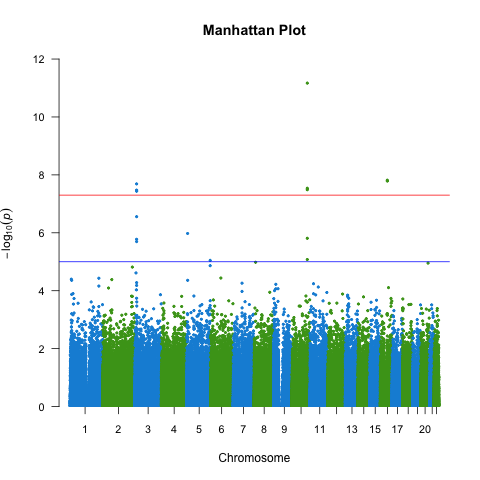
\includegraphics[width=0.85\linewidth]{img/_gwas_dummy/show-manhattan} 

}

\caption{A manhattan plot.}\label{fig:showmanhattan}
\end{figure}

\hypertarget{other-plots}{%
\section{Other plots}\label{other-plots}}

It is also informative to plot the density per chromosome. We can use the \passthrough{\lstinline!CMplot!} for that which you can find \href{https://github.com/YinLiLin/R-CMplot}{here}. For now we just make these graphs `quick-n-dirty', you can further prettify them, but you easily loose track of time, so maybe carry on.

\begin{quote}
Question: What do the grey spots on the density plot indicate?
\end{quote}

This would lead to the following graphs.

\begin{figure}[H]

{\centering 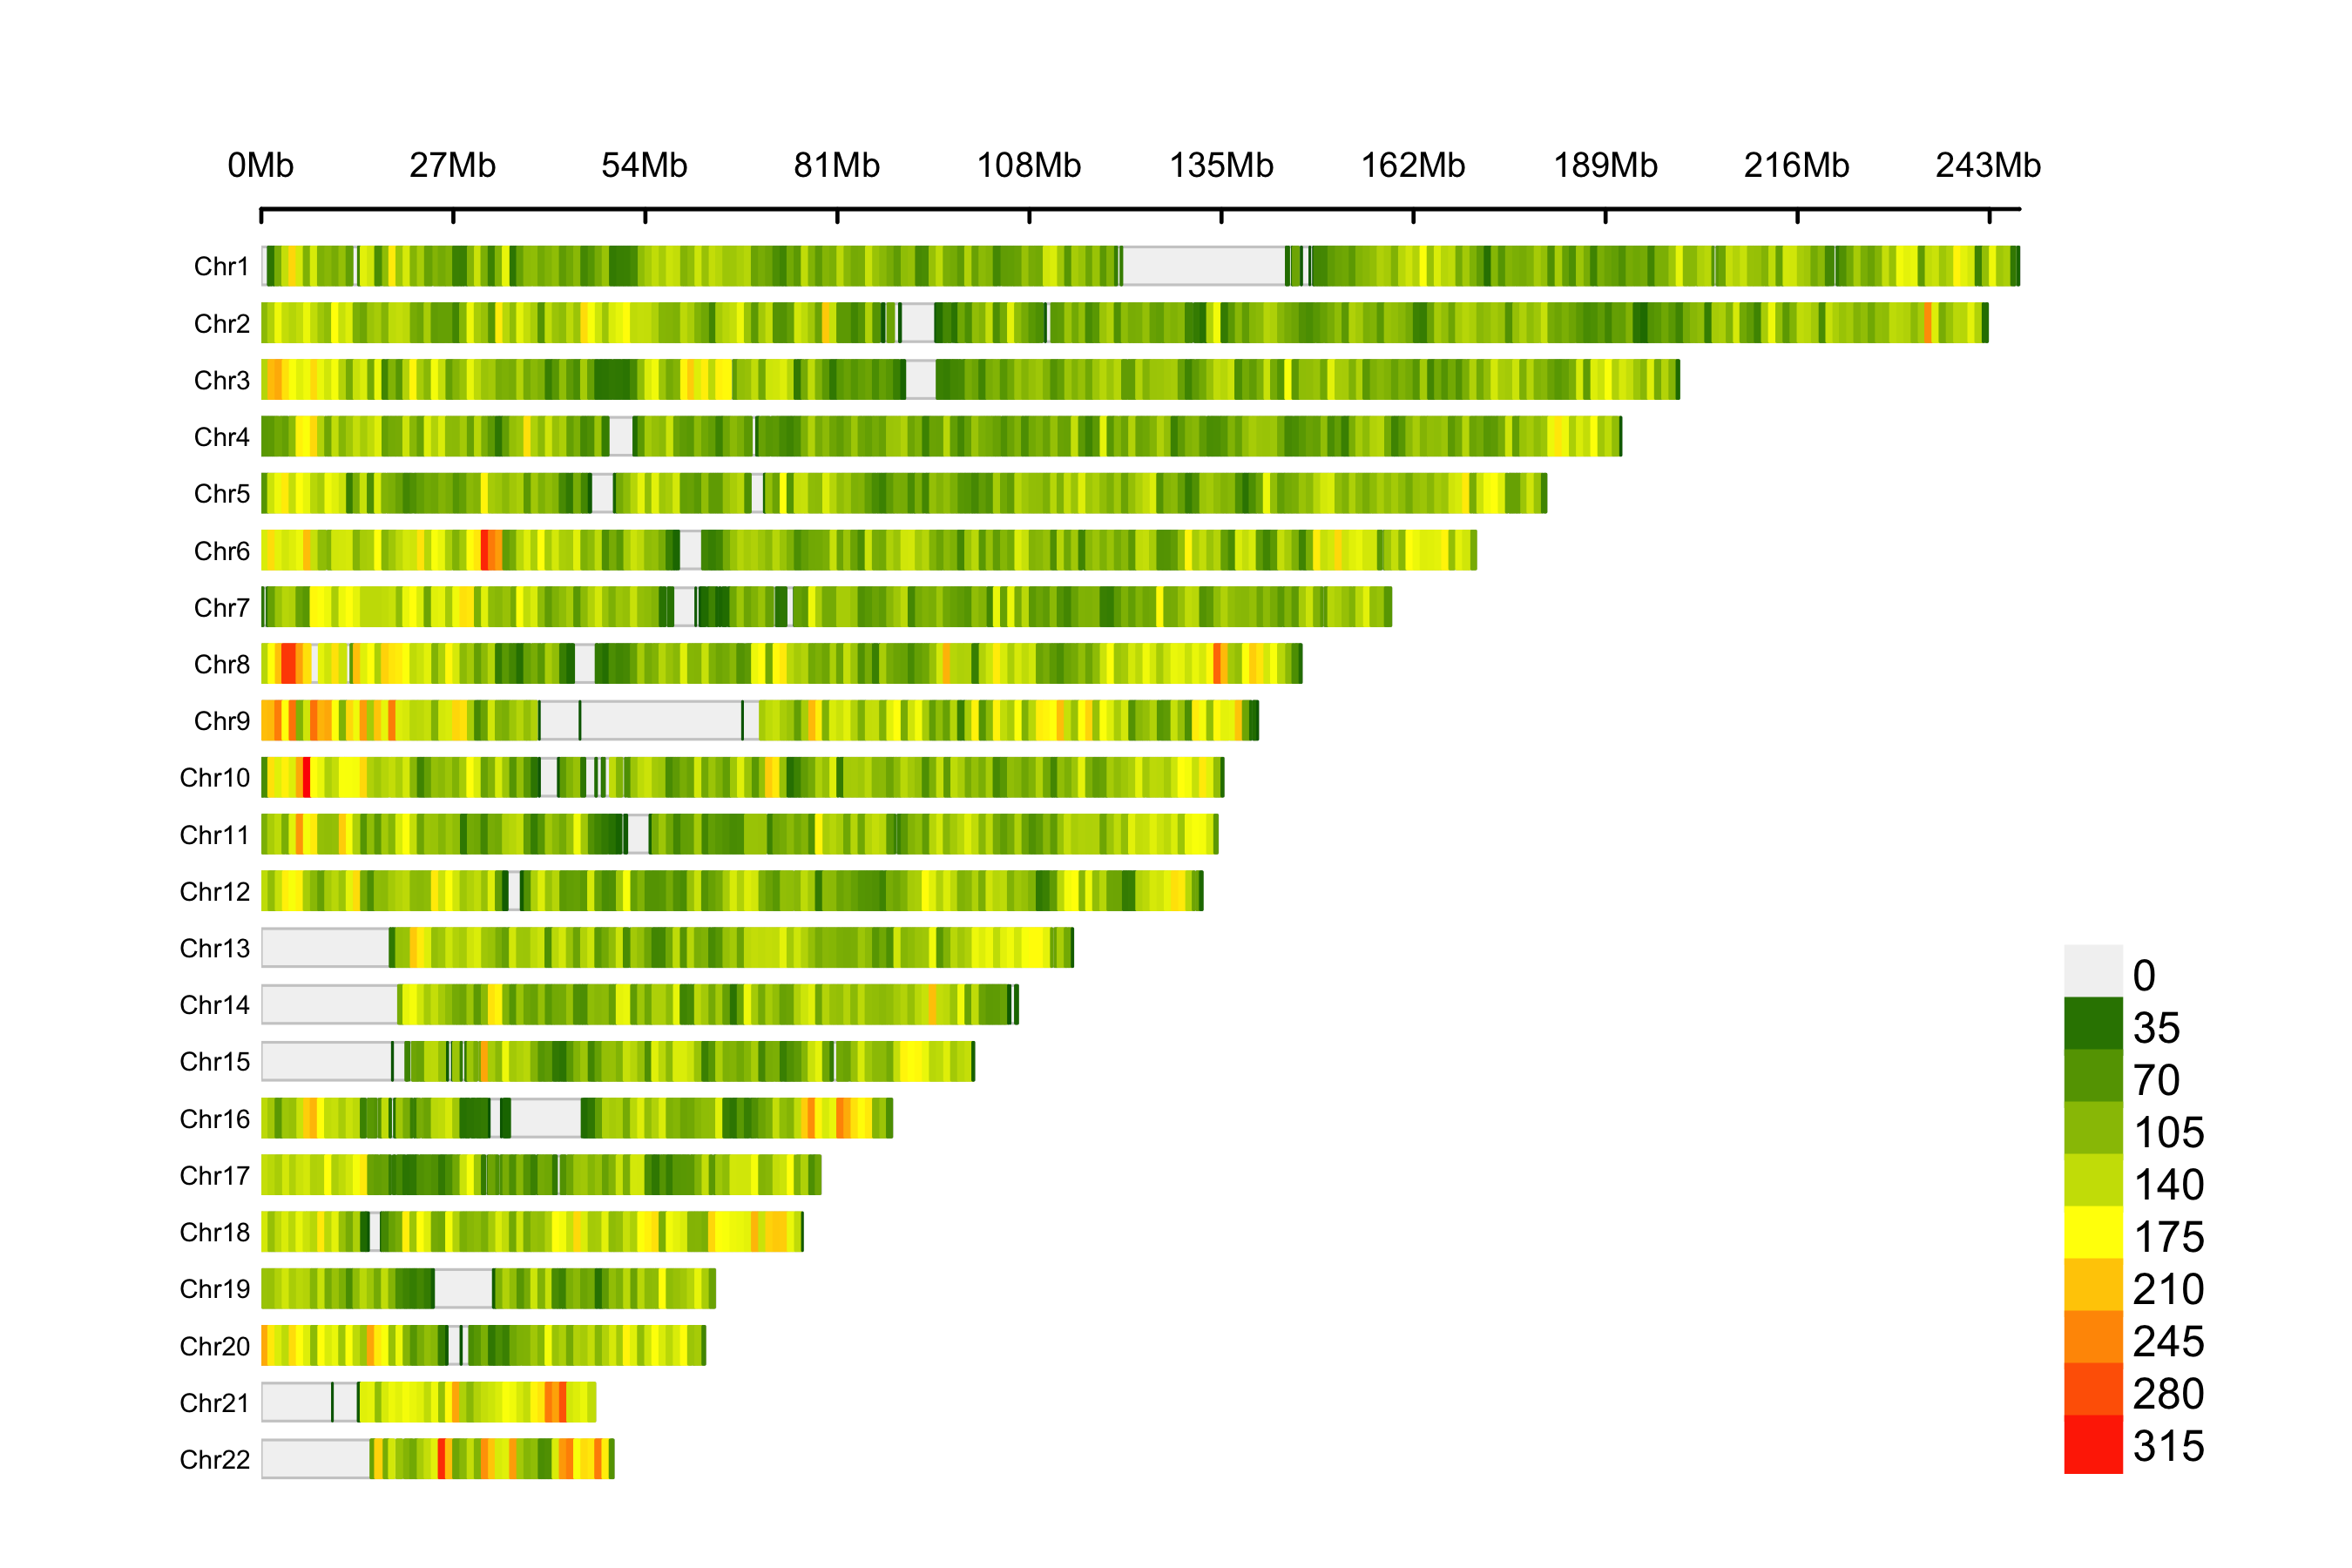
\includegraphics[width=0.85\linewidth]{img/_gwas_dummy/show-cmplot-all-density} 

}

\caption{SNP density of the association results.}\label{fig:showcmplotalldensity}
\end{figure}

\begin{figure}[H]

{\centering 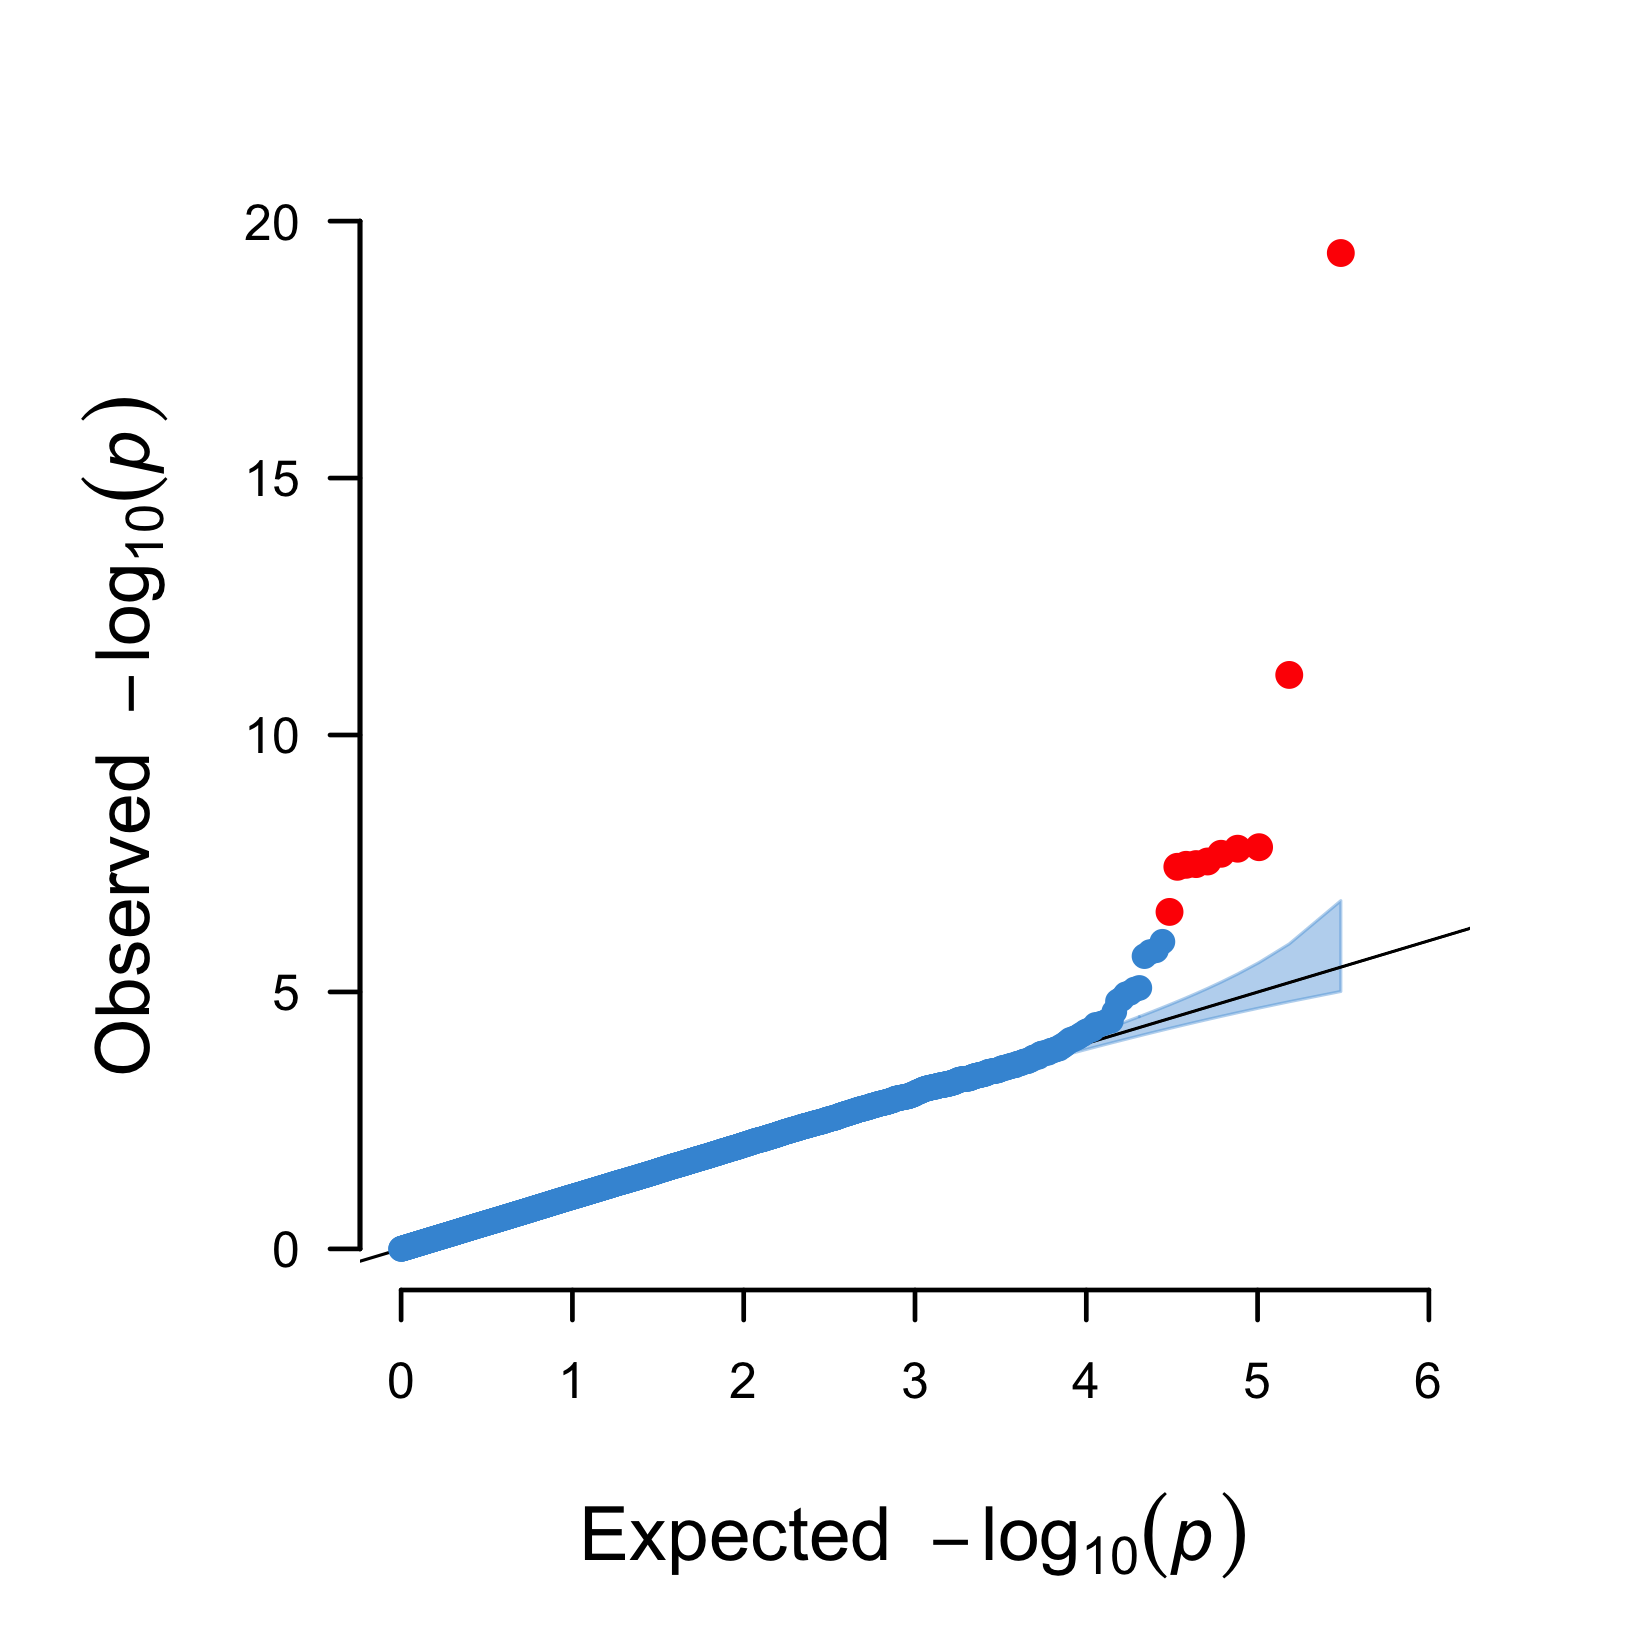
\includegraphics[width=0.85\linewidth]{img/_gwas_dummy/show-cmplot-all-qq} 

}

\caption{A QQ plot including a 95\% confidence interval (blue area) and genome-wide significant hits (red).}\label{fig:showcmplotallqq}
\end{figure}

\begin{figure}[H]

{\centering 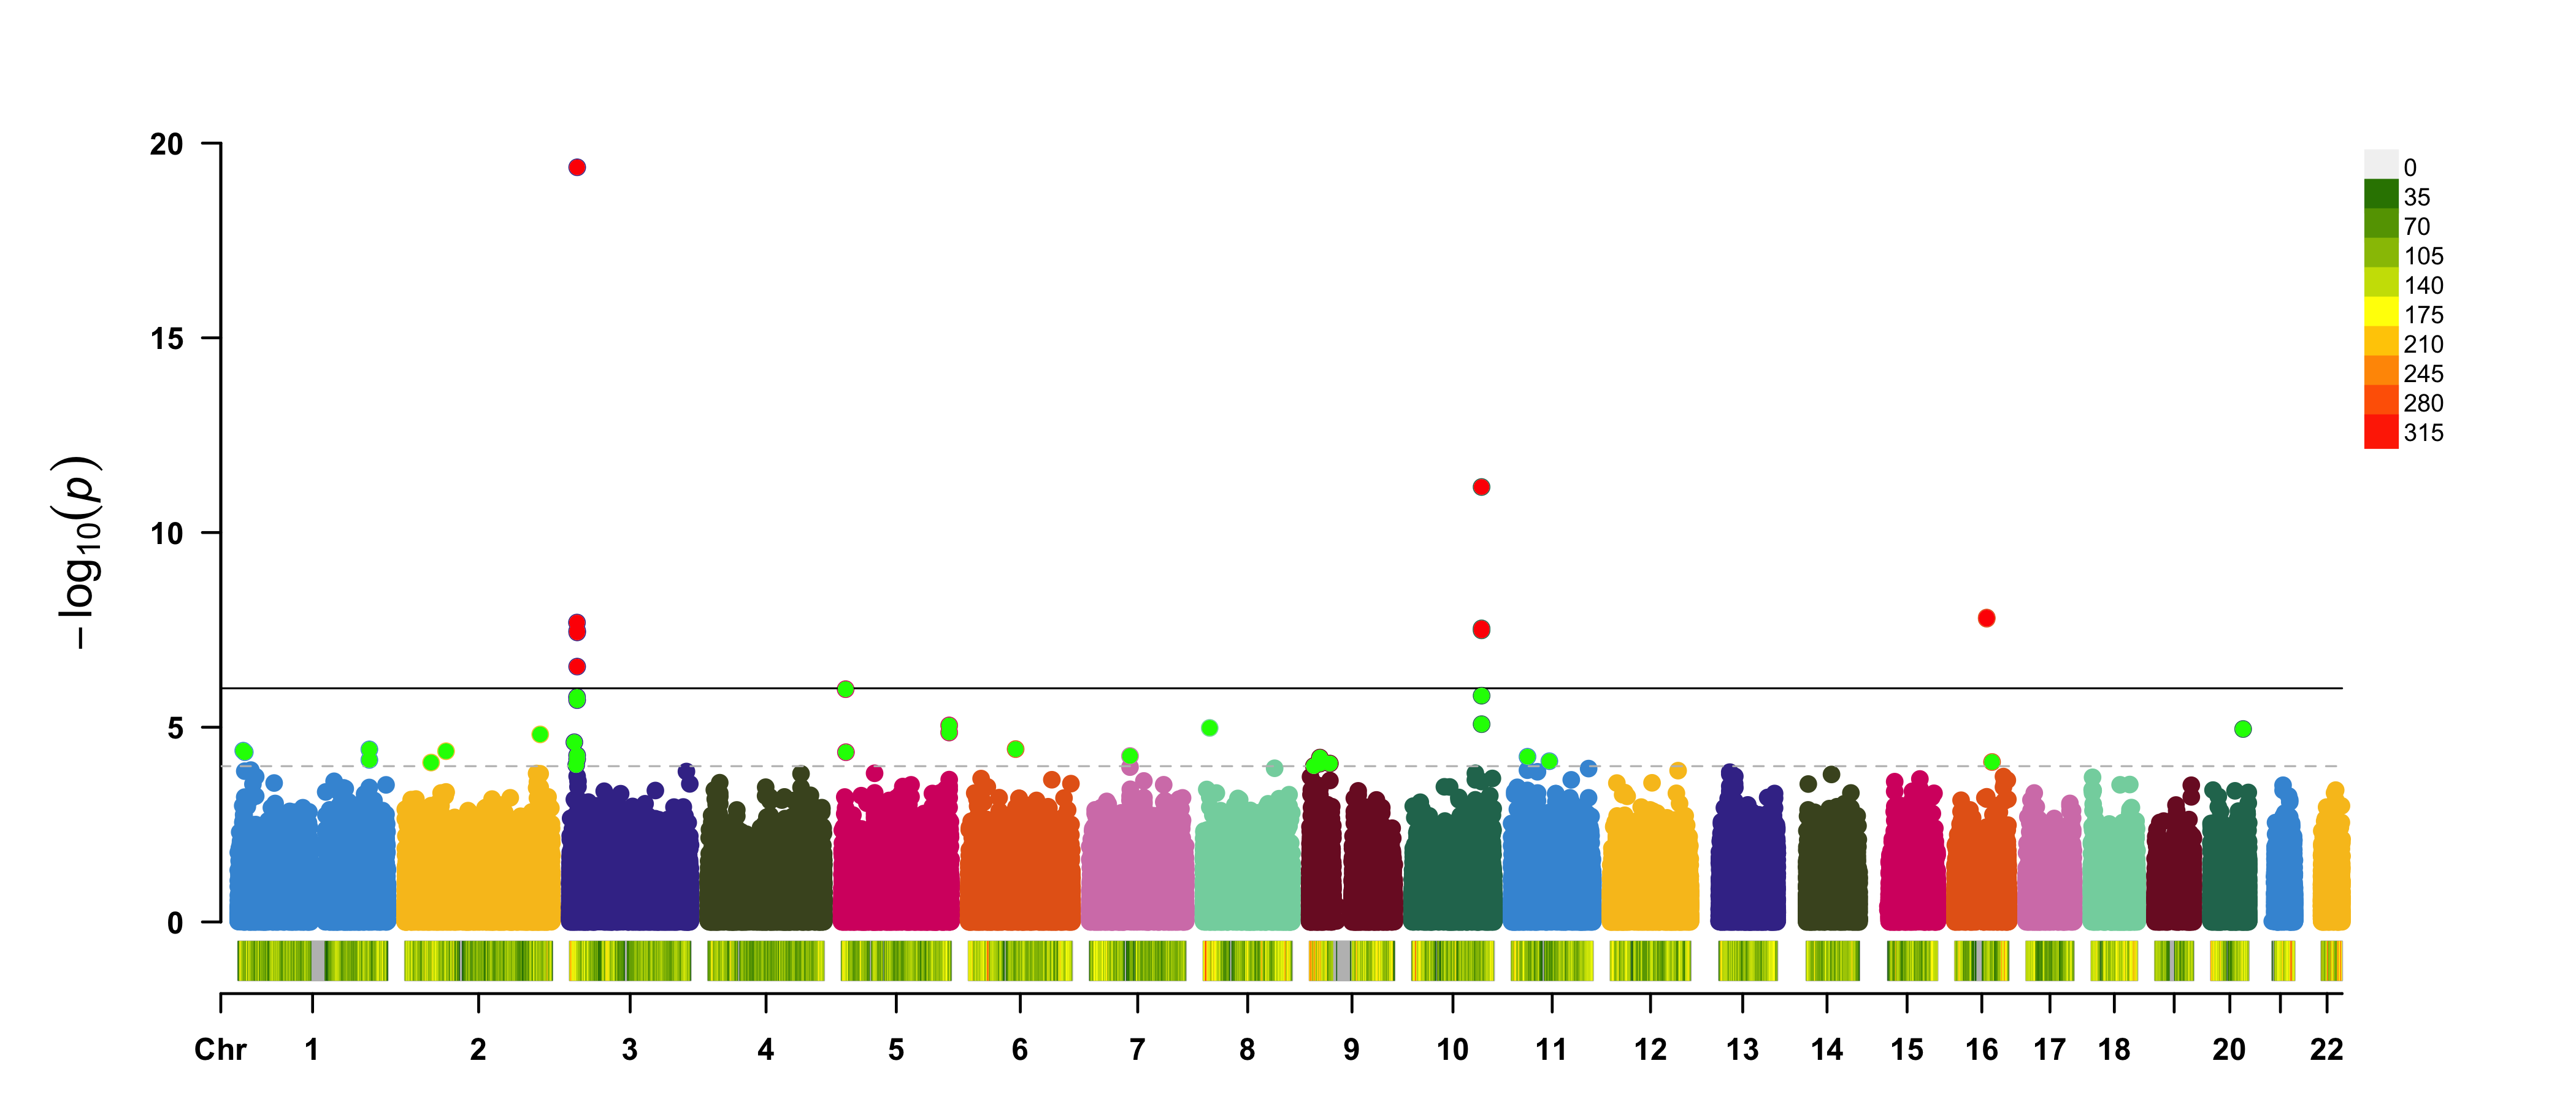
\includegraphics[width=0.85\linewidth]{img/_gwas_dummy/show-cmplot-all-manhattan} 

}

\caption{A regular manhattan plot. Colored by chromosome, suggestive hits are green, genome-wide hits are red. The bottom graph shows the per-chromosome SNP density.}\label{fig:showcmplotallmanhattan}
\end{figure}

\begin{figure}[H]

{\centering 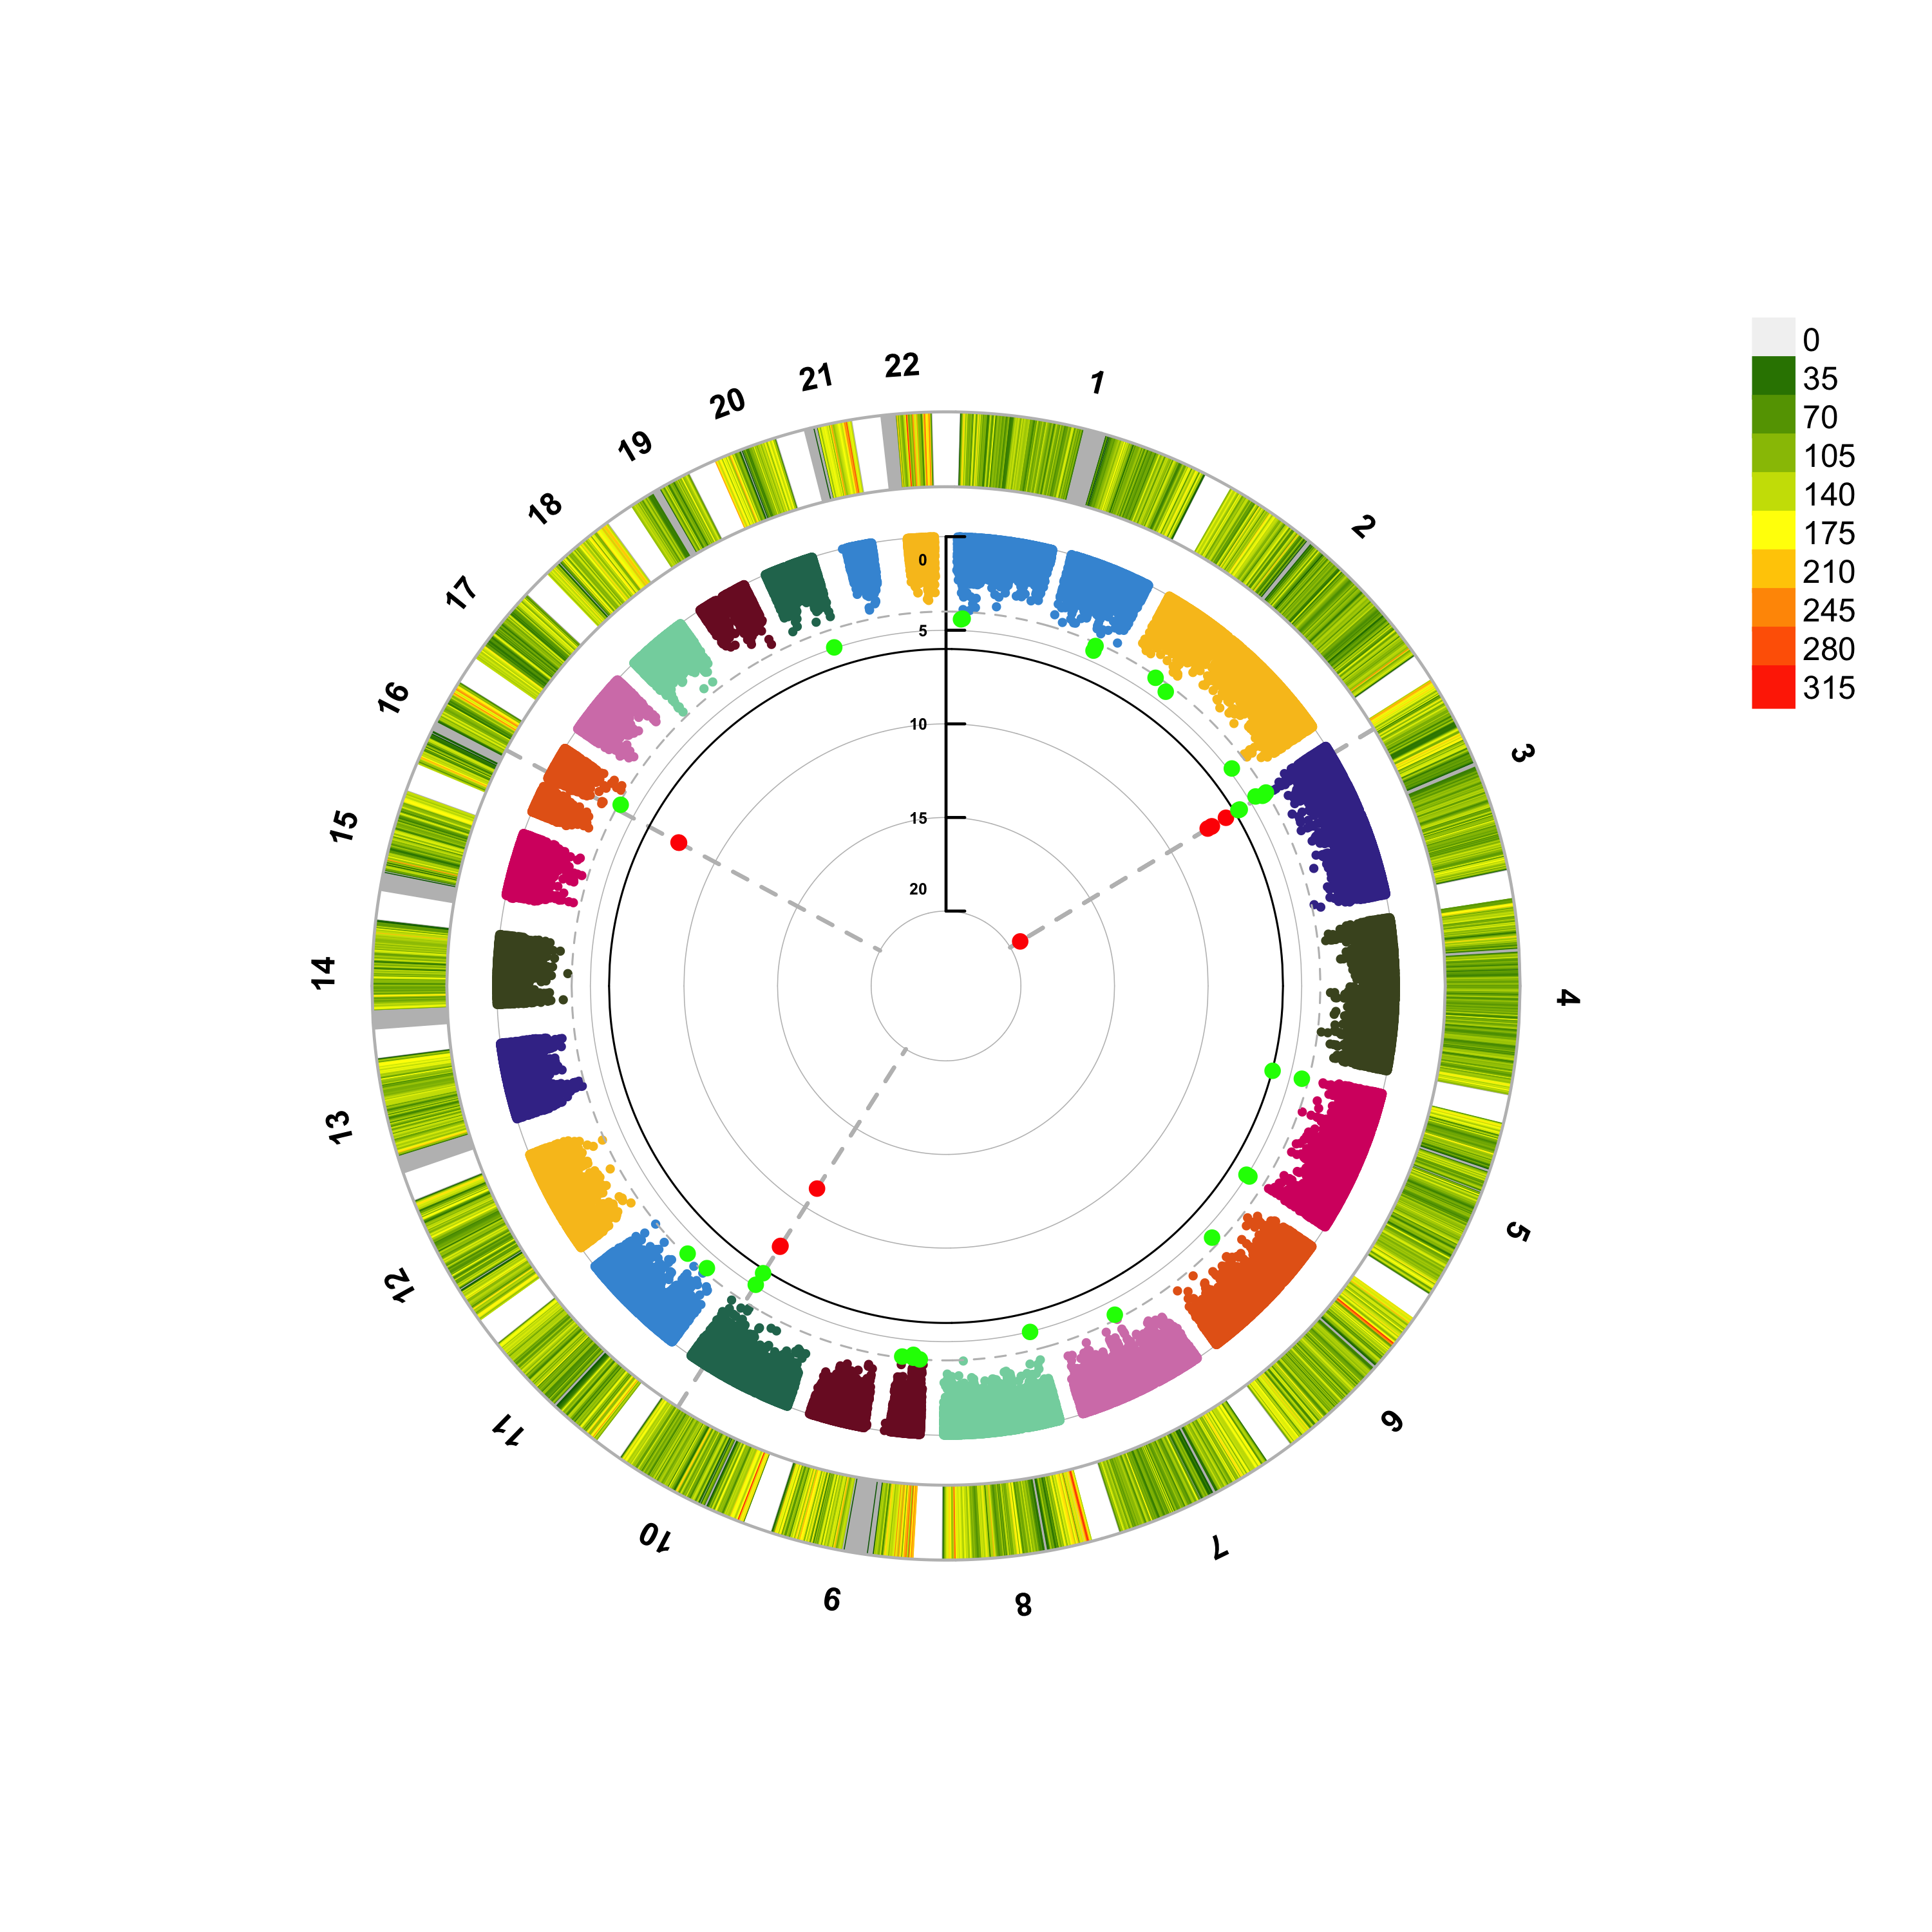
\includegraphics[width=0.85\linewidth]{img/_gwas_dummy/show-cmplot-all-circular} 

}

\caption{A circular manhattan.}\label{fig:show-cmplot-all-circular}
\end{figure}

\hypertarget{interactive-plots}{%
\section{Interactive plots}\label{interactive-plots}}

You can also make an \href{https://r-graph-gallery.com/101_Manhattan_plot.html}{interactive version} of the Manhattan - just because you can. The code below shows you how.

\begin{lstlisting}
library(plotly)
library(dplyr)

# Prepare the dataset (as an example we use the data (gwasResults) from the `qqman`-package)
don <- gwasResults %>%

  # Compute chromosome size
  group_by(CHR) %>%
  summarise(chr_len=max(BP)) %>%

  # Calculate cumulative position of each chromosome
  mutate(tot=cumsum(chr_len)-chr_len) %>%
  select(-chr_len) %>%

  # Add this info to the initial dataset
  left_join(gwasResults, ., by=c("CHR"="CHR")) %>%

  # Add a cumulative position of each SNP
  arrange(CHR, BP) %>%
  mutate( BPcum=BP+tot) %>%

  # Add highlight and annotation information
  mutate( is_highlight=ifelse(SNP %in% snpsOfInterest, "yes", "no")) %>%

  # Filter SNP to make the plot lighter
  filter(-log10(P)>0.5)

# Prepare X axis
axisdf <- don %>% group_by(CHR) %>% summarize(center=( max(BPcum) + min(BPcum) ) / 2 )

# Prepare text description for each SNP:
don$text <- paste("SNP: ", don$SNP, "\nPosition: ", don$BP, "\nChromosome: ", don$CHR, "\nLOD score:", -log10(don$P) %>% round(2), "\nWhat else do you wanna know", sep="")

# Make the plot
p <- ggplot(don, aes(x=BPcum, y=-log10(P), text=text)) +

    # Show all points
    geom_point( aes(color=as.factor(CHR)), alpha=0.8, size=1.3) +
    scale_color_manual(values = rep(c("grey", "skyblue"), 22 )) +

    # custom X axis:
    scale_x_continuous( label = axisdf$CHR, breaks= axisdf$center ) +
    scale_y_continuous(expand = c(0, 0)) +     # remove space between plot area and x axis

    # Add highlighted points
    geom_point(data=subset(don, is_highlight=="yes"), color="orange", size=2) +

    # Custom the theme:
    theme_bw() +
    theme(
      legend.position="none",
      panel.border = element_blank(),
      panel.grid.major.x = element_blank(),
      panel.grid.minor.x = element_blank()
    )
ggplotly(p, tooltip="text")
\end{lstlisting}

It will produce something like this.

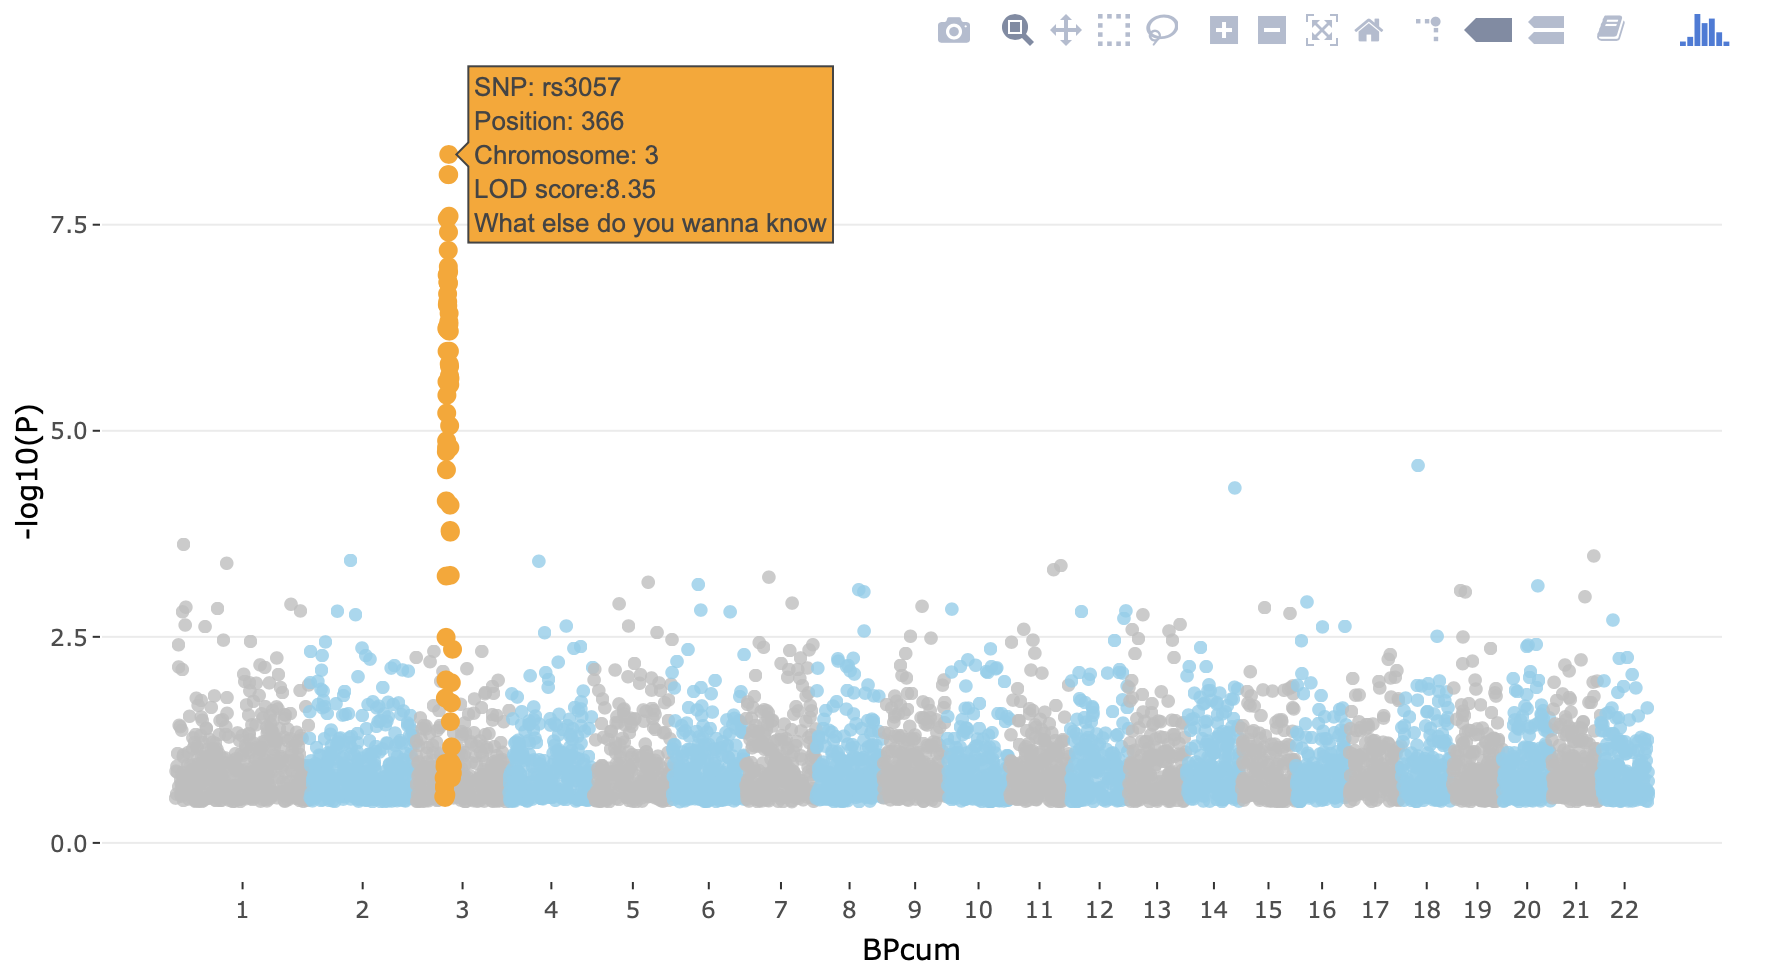
\includegraphics{img/_gwas/interactive_plot.png}

Again, this is an example with dummy data - you can try to do it for our GWAS, but careful with the time. You can also choose to carry on.

You will encounter the above types of visualizations in any high-quality GWAS paper, because each is so critically informative. Usually, analysts of large-scale meta-analyses of GWAS will also stratify the QQ-plots based on the imputation quality (if your GWAS was imputed), call rate, and allele frequency (although that is rarely shared in publications, not even in supplemental material).

\hypertarget{stop-playing-around}{%
\section{Stop playing around}\label{stop-playing-around}}

Alright. It's time to stop playing around and do a quick recap of what you've learned.

\begin{enumerate}
\def\labelenumi{\arabic{enumi}.}
\tightlist
\item
  You learned how to convert datasets.
\item
  You learned how to execute sample QC and create diagnostic graphics
\item
  You learned how to do the same for SNP QC
\item
  You learned how to execute an association study given a dataset, covariates, and different assumptions regarding the genetic model.
\item
  You learned how to visualize results and played around with different visuals.
\end{enumerate}

You should be ready for the real stuff. And if not, the next chapter will help you get ready: Chapter @ref(wtccc1\_intro).

\hypertarget{wtccc1_intro}{%
\chapter{The Welcome Trust Case-Control Consortium}\label{wtccc1_intro}}

Now that you know your way around \passthrough{\lstinline!PLINK!}, \passthrough{\lstinline!bash!} and \passthrough{\lstinline!r!} and have done some basic quality control and association testing, you are ready for the real thing. We have prepared a real dataset: the first release of the \href{https://www.wtccc.org.uk/ccc1/overview.html}{\emph{Welcome Trust Case-Control Consortium (WTCCC)}} on coronary artery disease (CAD) and a control dataset used for that project.

\hypertarget{genotyping}{%
\section{Genotyping}\label{genotyping}}

The WTCCC1 data were genotyped using a chip from \href{https://www.thermofisher.com/us/en/home/life-science/microarray-analysis/affymetrix.html?category=34000\&categoryIdClicked=34000\&rootCategoryId=34000\&navMode=34000\&aId=productsNav}{Affymetrix}, nowadays part of ThermoFisher. As a brand Affymetrix still exists, but the chips aren't made anymore. Unfortunately, most links to the old generation Affymetrix chips are borken, but you can still find some information about the 500K chip that was used for \href{https://tools.thermofisher.com/content/sfs/brochures/whole_genome_assoc_500k_jsmith.pdf}{WTCCC1}. It's good practice to read up a bit on what chip was used, and what \href{https://www.thermofisher.com/us/en/home/life-science/microarray-analysis/microarray-data-analysis.html}{support materials are available}.

\hypertarget{the-data}{%
\section{The data}\label{the-data}}

Before quality control the original data included:

\begin{itemize}
\tightlist
\item
  CAD cohort, n ± 2,000
\item
  Healthy controls, from the UK 1958 birth control cohort, n ± 1,500 (we won't use this)
\item
  Healthy controls, from the UK National Blood Service, n ± 1,500.
\end{itemize}

\hypertarget{assignment}{%
\section{Assignment}\label{assignment}}

Your assignment in the next chapter (Chapter \ref{wtccc1}) is to do the following:

\begin{enumerate}
\def\labelenumi{\arabic{enumi}.}
\tightlist
\item
  Explore the individual datasets by calculating some statistics and visualising these.
\item
  Merge the datasets in the folder \passthrough{\lstinline!wtccc1!}.
\item
  Calculate PCs using smartPCA.
\item
  Perform an association test using available covariates.
\item
  Visualize the results.
\item
  Identify independent SNPs.
\item
  Make regional association plots.
\end{enumerate}

\hypertarget{there-you-go}{%
\section{There you go}\label{there-you-go}}

As I wrote, you are ready for the real stuff in Chapter \ref{wtccc1}.

\hypertarget{wtccc1}{%
\chapter{WTCCC1: a GWAS on coronary artery disease (CAD)}\label{wtccc1}}

As usual, we start by exploring the data in hand.

\begin{lstlisting}
plink --bfile wtccc1/CADn1871_500Kb37fwd --bmerge wtccc1/UKBSn1397_500Kb37fwd --make-bed --out wtccc1/wtccc1 && \
plink --bfile wtccc1/wtccc1 --freq --out wtccc1/wtccc1 && \
plink --bfile wtccc1/wtccc1 --hardy --out wtccc1/wtccc1 && \
plink --bfile wtccc1/wtccc1 --missing --out wtccc1/wtccc1 && \
plink --bfile wtccc1/wtccc1 --test-missing --out wtccc1/wtccc1

cat wtccc1/wtccc1.missing | awk '$5 < 0.00001' | awk '{ print $2 }' > wtccc1/wtccc1-fail-diffmiss-qc.txt
\end{lstlisting}

Let's investigate the HWE p-value in the whole cohort, and per stratum (cases and controls) with the code below.

This will result in Figure \ref{fig:show-wtccc1-hwe}.

\begin{figure}[H]

{\centering 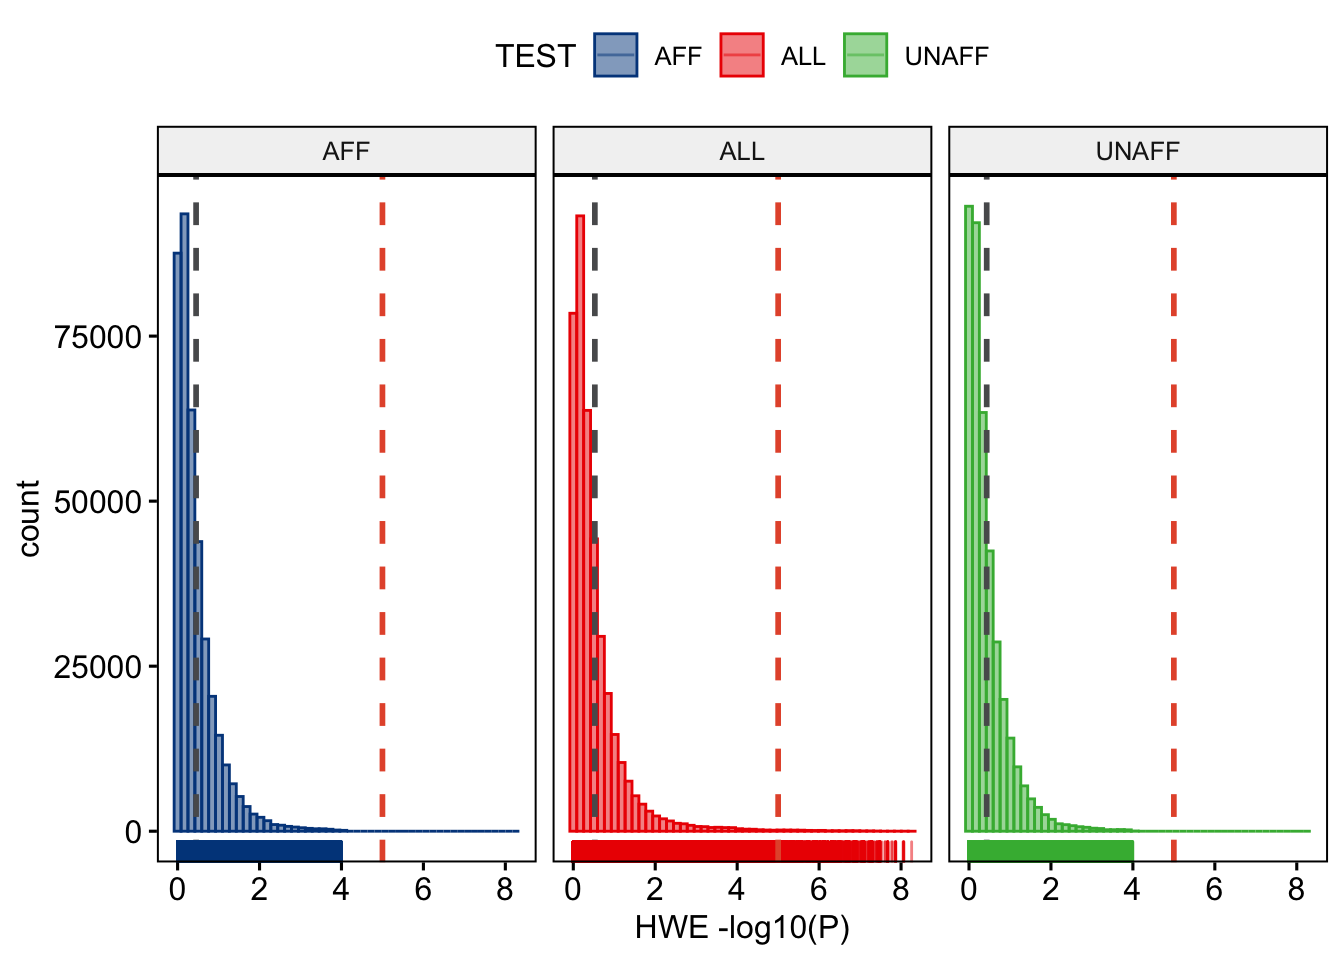
\includegraphics[width=0.85\linewidth]{img/_gwas_wtccc/WTCCC1-HWE} 

}

\caption{Stratified HWE p-values.}\label{fig:show-wtccc1-hwe}
\end{figure}

We should also inspect the allele frequencies. Note that \emph{by default} PLINK (whether v0.7, v1.9, or v2.0) stores the alleles as minor (A1) and major (A2), and therefore \passthrough{\lstinline!--maf!} \emph{always} calculates the frequency of the minor allele (A1).

This will result in Figure \ref{fig:show-wtccc1-freq}.

\begin{figure}[H]

{\centering 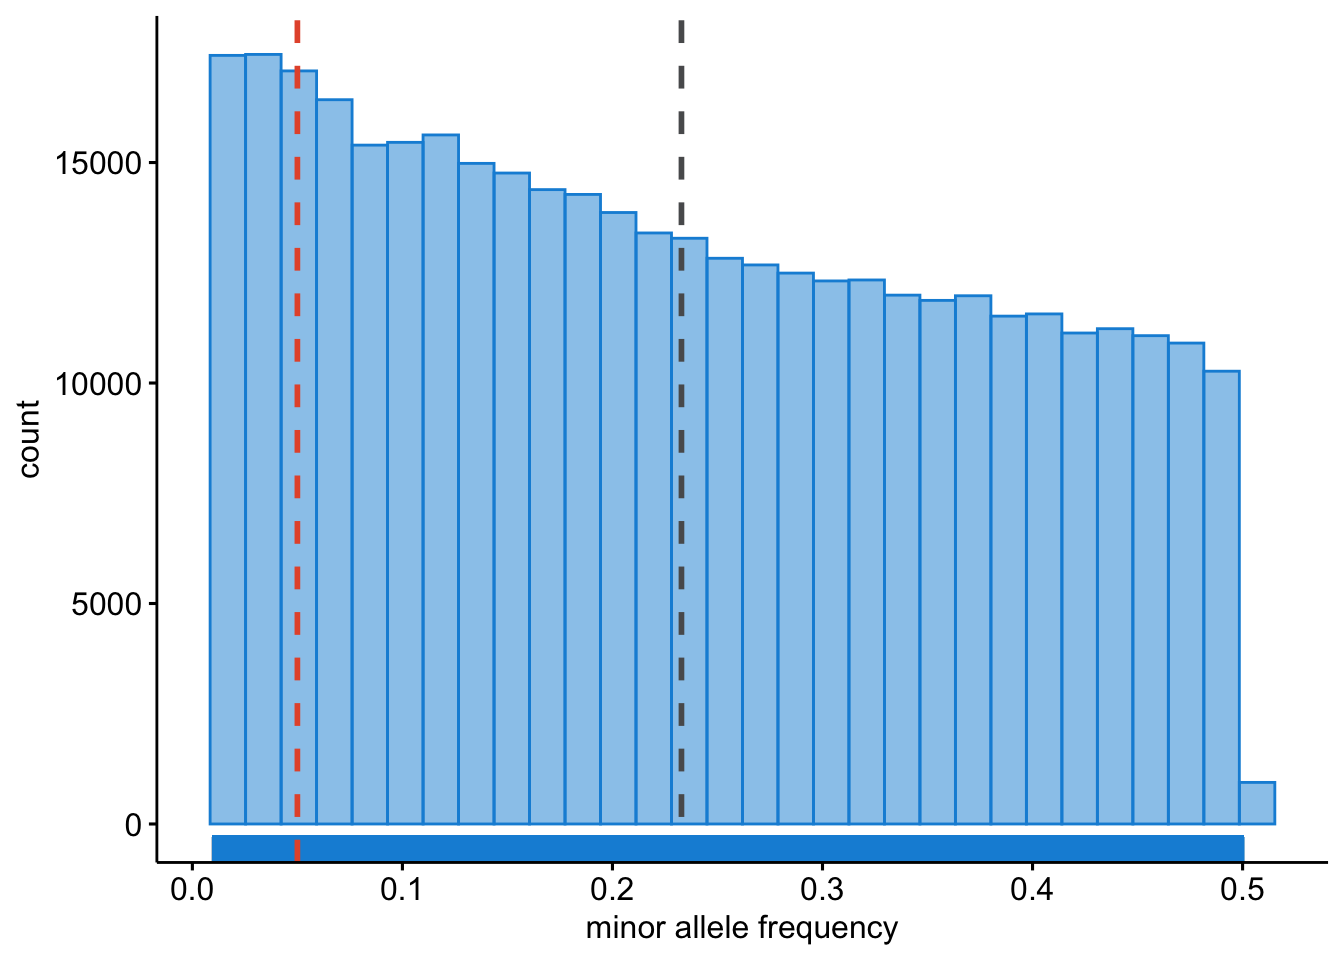
\includegraphics[width=0.85\linewidth]{img/_gwas_wtccc/WTCCC1-FREQ} 

}

\caption{Minor allele frequencies.}\label{fig:show-wtccc1-freq}
\end{figure}

There could be sample with very poor overall call rate, where for many SNPs there is no data. We will want to identify these samples and exclude them.

This will result in Figure \ref{fig:show-wtccc1-callratesample}.

\begin{figure}[H]

{\centering 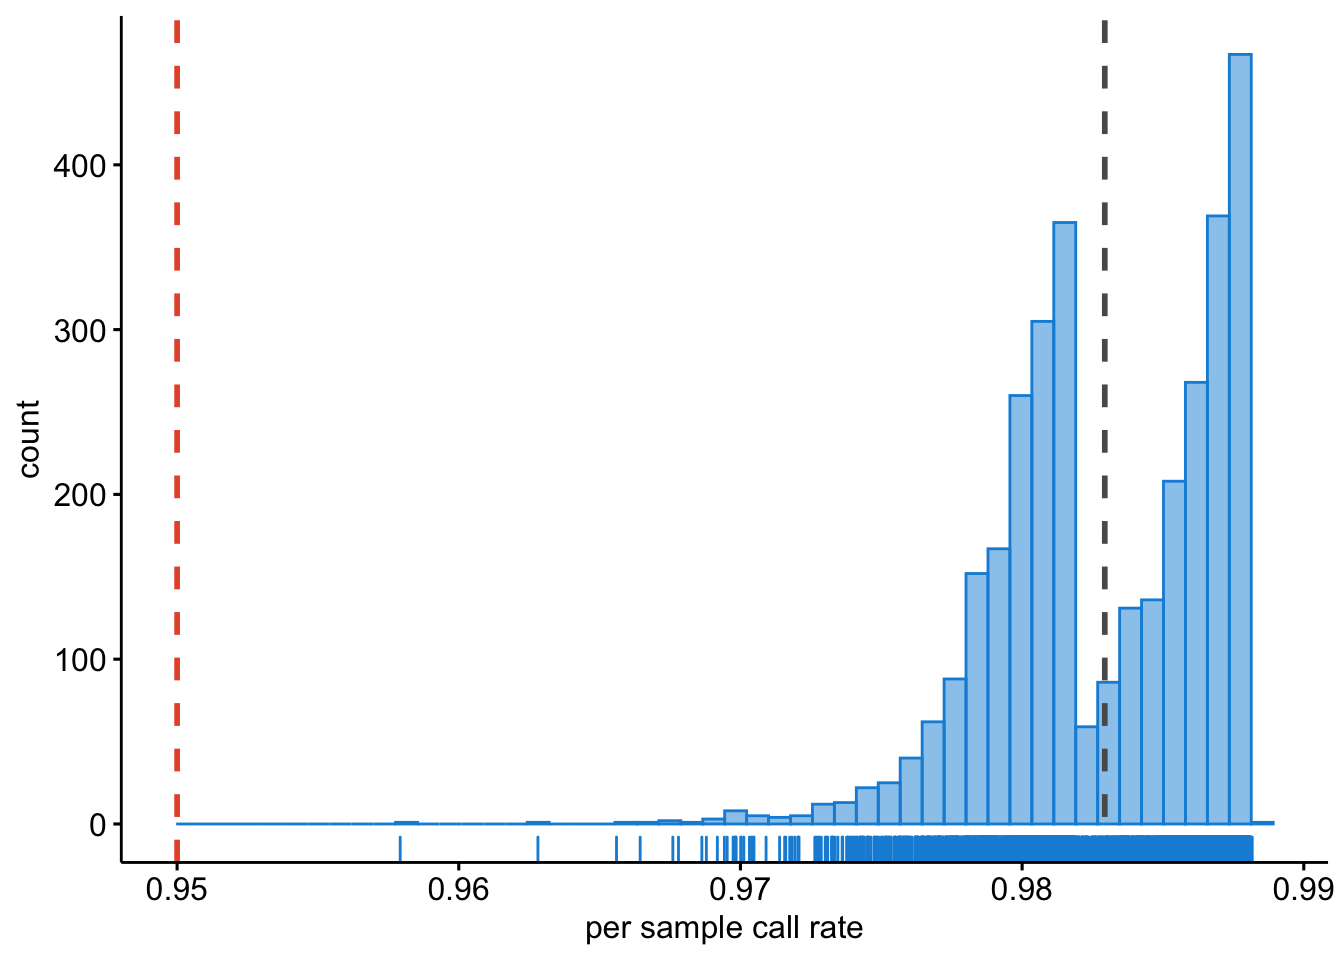
\includegraphics[width=0.85\linewidth]{img/_gwas_wtccc/WTCCC1-callrate-samples} 

}

\caption{Per sample call rate.}\label{fig:show-wtccc1-callratesample}
\end{figure}

Lastly, we must inspect the per SNP call rate; we need to know if there are SNPs that have no data for many samples. We will want to identify such SNPs and exclude these.

This will result in Figure \ref{fig:show-wtccc1-callratesnp}.

\begin{figure}[H]

{\centering 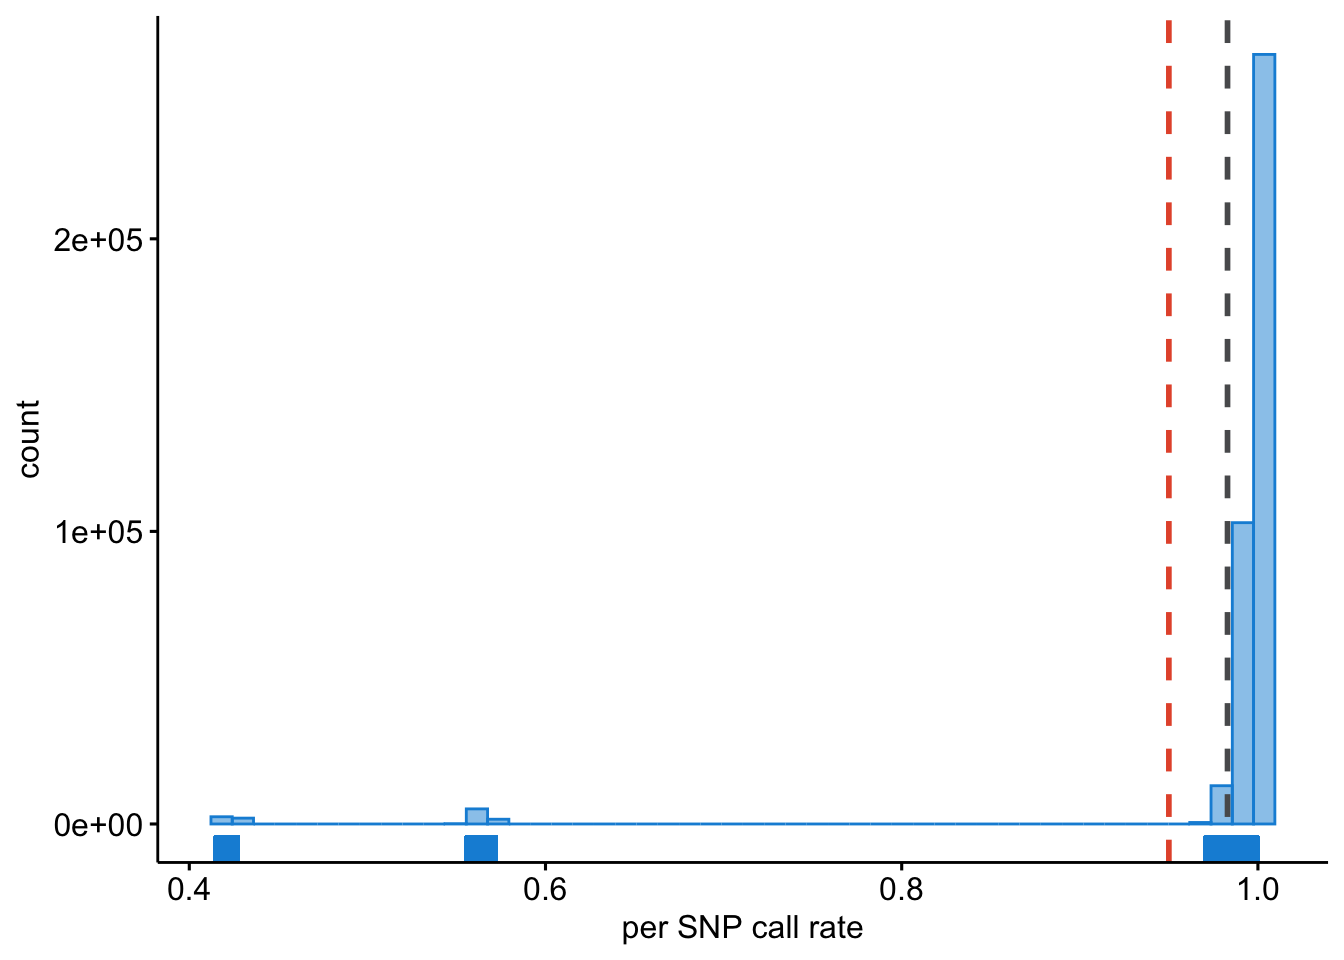
\includegraphics[width=0.85\linewidth]{img/_gwas_wtccc/WTCCC1-callrate-SNPs} 

}

\caption{Per SNP call rate.}\label{fig:show-wtccc1-callratesnp}
\end{figure}

\hypertarget{quality-control-1}{%
\section{Quality control}\label{quality-control-1}}

Now that we have handle on the data, we can filter it.

\begin{quote}
Do you have any thoughts on that? Do you agree with the filters I set below? How would you do it differently and why?
\end{quote}

\begin{lstlisting}
plink --bfile wtccc1/wtccc1 --exclude wtccc1/wtccc1-fail-diffmiss-qc.txt --maf 0.01 --geno 0.05 --hwe 0.00001 --make-bed --out wtccc1/wtccc1_clean
\end{lstlisting}

\hypertarget{ancestral-background-1}{%
\section{Ancestral background}\label{ancestral-background-1}}

If these individuals are all from the United Kingdom, we are certain there will be admixture from other populations given UK's history. Let's project the WTCCC1 data on 1000G phase 1 populations.

We will face the same issue as before with our dummy dataset with respect to \passthrough{\lstinline!EIGENSOFT!}. So I created the data for you to skip to the \protect\hyperlink{plotting-pca}{Plotting PCA} section immediately. Regardless, in the \protect\hyperlink{preparing-pca}{Preparing PCA} and \protect\hyperlink{running-pca}{Running PCA} sections I show you how to get there.

\hypertarget{preparing-pca}{%
\subsection{Preparing PCA}\label{preparing-pca}}

\textbf{Filtering WTCCC1}

For PCA we need to perform extreme clean.

\begin{lstlisting}
plink --bfile wtccc1/wtccc1_clean --maf 0.1 --geno 0.1 --indep-pairwise 100 50 0.2 --exclude support/exclude_problematic_range.txt --make-bed --out wtccc1/wtccc1_temp

plink --bfile wtccc1/wtccc1_temp --exclude wtccc1/wtccc1_temp.prune.out --make-bed --out wtccc1/wtccc1_extrclean

rm -fv wtccc1/wtccc1_temp*

cat wtccc1/wtccc1_extrclean.bim | awk '{ print $2 }' > wtccc1/wtccc1_extrclean.variants.txt

cat wtccc1/wtccc1.bim | grep "rs" > wtccc1/all.variants.txt
\end{lstlisting}

\textbf{Merging WTCCC1 with 1000G phase 1}

Now we are ready to extract the WTCCC1 variants from the 1000G phase 1 reference

\begin{lstlisting}
plink --bfile ref_1kg_phase1_all/1kg_phase1_all --extract wtccc1/all.variants.txt --make-bed --out ref_1kg_phase1_all/1kg_phase1_wtccc1
\end{lstlisting}

Extracting the A/T and C/G SNPs as well.

\begin{lstlisting}
cat ref_1kg_phase1_all/1kg_phase1_wtccc1.bim | \
awk '($5 == "A" && $6 == "T") || ($5 == "T" && $6 == "A") || ($5 == "C" && $6 == "G") || ($5 == "G" && $6 == "C")' | awk '{ print $2, $1, $4, $3, $5, $6 }' \
> ref_1kg_phase1_all/all.1kg_wtccc1.atcg.variants.txt
\end{lstlisting}

\begin{lstlisting}
plink --bfile ref_1kg_phase1_all/1kg_phase1_wtccc1 --exclude ref_1kg_phase1_all/all.1kg_wtccc1.atcg.variants.txt --make-bed --out ref_1kg_phase1_all/1kg_phase1_wtccc1_no_atcg

plink --bfile ref_1kg_phase1_all/1kg_phase1_wtccc1_no_atcg --extract wtccc1/wtccc1_extrclean.variants.txt --make-bed --out ref_1kg_phase1_all/1kg_phase1_raw_no_atcg_wtccc1
\end{lstlisting}

Finally we will merge the datasets.

\begin{lstlisting}
plink --bfile wtccc1/wtccc1_extrclean --bmerge ref_1kg_phase1_all/1kg_phase1_raw_no_atcg_wtccc1 --maf 0.1 --geno 0.1 --exclude support/exclude_problematic_range.txt --make-bed --out wtccc1/wtccc1_extrclean_1kg
\end{lstlisting}

\hypertarget{running-pca}{%
\subsection{Running PCA}\label{running-pca}}

\begin{lstlisting}
cp -v wtccc1/wtccc1_extrclean_1kg.bim wtccc1/wtccc1_extrclean_1kg.pedsnp
cp -v wtccc1/wtccc1_extrclean_1kg.fam wtccc1/wtccc1_extrclean_1kg.pedind
\end{lstlisting}

Now that the cleaning is done, we can execute the actual PCA.

\begin{lstlisting}
perl ~/git/EIG/bin/smartpca.perl \
-i wtccc1/wtccc1_extrclean_1kg.bed \
-a wtccc1/wtccc1_extrclean_1kg.pedsnp \
-b wtccc1/wtccc1_extrclean_1kg.pedind \
-k 10 \
-o wtccc1/wtccc1_extrclean_1kg.pca \
-p wtccc1/wtccc1_extrclean_1kg.plot \
-e wtccc1/wtccc1_extrclean_1kg.eval \
-l wtccc1/wtccc1_extrclean_1kg.log \
-m 5 \
-t 10 \
-s 6.0 \
-w ref_1kg_phase1_all/1kg-pca-populations.txt
\end{lstlisting}

\hypertarget{plotting-pca}{%
\subsection{Plotting PCA}\label{plotting-pca}}

If all is peachy, you were able to run the PCA for the WTCCC1 data against 1000G phase 1. Using \passthrough{\lstinline!smartpca!} (you know, \passthrough{\lstinline!EIGENSOFT!}) we have calculated principal components (PCs) and we can now start plotting them. Let's create a scatter diagram of the first two principal components, including all individuals in the file \passthrough{\lstinline!wtccc1\_extrclean\_1kg.pca.evec!} (the first and second principal components are columns 2 and 3, respectively). Use the data in column 4 to color the points according to sample origin.

\begin{quote}
Please note! You may have been able to make \passthrough{\lstinline!EIGENSOFT!} to work. So you may have to change ``/ref\_pca\_wtccc1/wtccc1\_extrclean\_1kg.pca.evec'' to ``/wtccc1/wtccc1\_extrclean\_1kg.pca.evec'' in the command below.
\end{quote}

And we should visualize the PCA results: are these individuals really all from European (UK) ancestry?

We expect most individuals from the WTCCC to be 100\% British, but a substantial group will have a different ancestral background as shown in the Figure \ref{fig:showwtccc1pca} you just made.

\begin{figure}[H]

{\centering 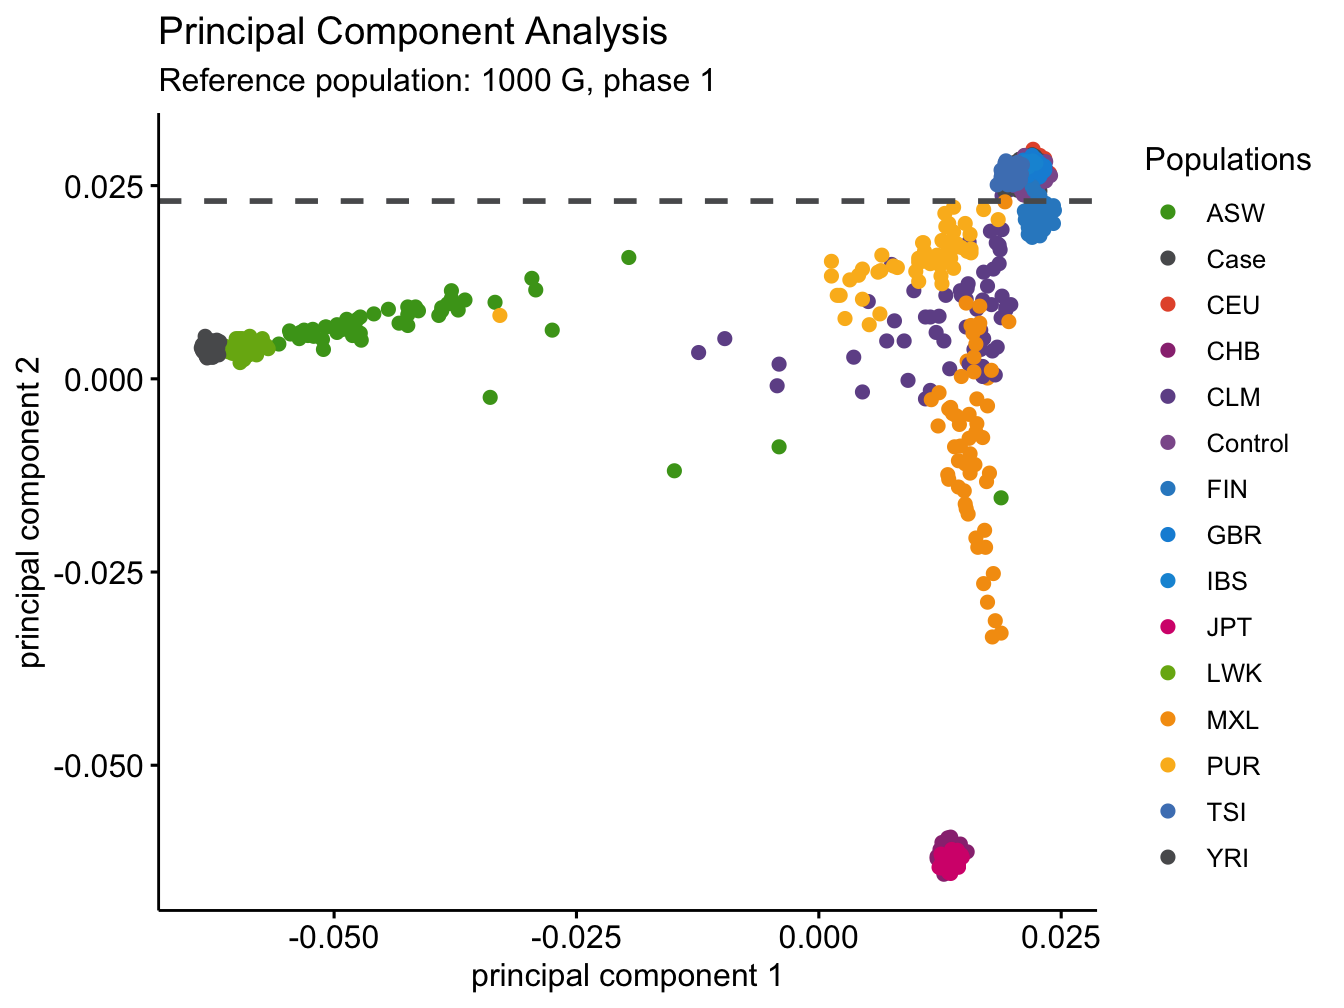
\includegraphics[width=0.85\linewidth]{img/_gwas_wtccc/WTCCC1-pca-1000g} 

}

\caption{PCA - WTCCC1 vs. 1000G}\label{fig:showwtccc1pca}
\end{figure}

\hypertarget{removing-samples-1}{%
\subsection{Removing samples}\label{removing-samples-1}}

In a similar fashion as in the example \emph{gwas} and \emph{rawdata} datasets, you should consider to \textbf{remove the samples below the threshold} based on this PCA (Figure \ref{fig:showwtccc1pca}).

\begin{quote}
Go ahead, try that.
\end{quote}

You're code would be something like below:

\begin{lstlisting}
cat wtccc1/wtccc1_extrclean_1kg.pca.evec | tail -n +2 | \
awk '$3 < 0.023' | awk '{ print $1 }' | awk -F":" '{ print $1, $2 }' > wtccc1/fail-ancestry-QC.txt
\end{lstlisting}

Next we filter these samples and get a final fully QC'd dataset.

\begin{lstlisting}
plink --bfile wtccc1/wtccc1_clean --exclude wtccc1/fail-ancestry-QC.txt --make-bed --out wtccc1/wtccc1_qc
\end{lstlisting}

\hypertarget{association-testing}{%
\section{Association testing}\label{association-testing}}

Now that we have explored the data, we are ready for some simple association testing. However, it would be great to have some PCs to correct for. We can use PLINK for that too.

\begin{lstlisting}
plink --bfile wtccc1/wtccc1_extrclean --exclude wtccc1/fail-ancestry-QC.txt --pca --out wtccc1/wtccc1_extrclean
\end{lstlisting}

Let's add those PCs to the covariates-file.

\begin{lstlisting}
echo "IID PC1 PC2 PC3 PC4 PC5 PC6 PC7 PC8 PC9 PC10 PC11 PC12 PC13 PC14 PC15 PC16 PC17 PC18 PC19 PC20" > wtccc1/wtccc1_qc.pca

cat wtccc1/wtccc1_extrclean.eigenvec | awk '{ print $2,$3,$4,$5,$6,$7,$8,$9,$10,$11,$12,$13,$14,$15,$16,$17,$18,$19,$20,$21,$22}' >> wtccc1/wtccc1_qc.pca

perl scripts/mergeTables.pl --file1 wtccc1/wtccc1_qc.pca --file2 wtccc1/wtccc1.covar --index IID --format NORM > wtccc1/wtccc1_qc.covar_pca
\end{lstlisting}

Exciting, now we are ready to perform a GWAS on CAD in WTCCC1.

\begin{lstlisting}
plink --bfile wtccc1/wtccc1_qc --logistic sex --covar wtccc1/wtccc1_qc.covar_pca --out wtccc1/wtccc1_qc_log_covar_pca
\end{lstlisting}

After you ran the association analysis, you're ready to process the data and take a first look at the results. First, we prepare the raw output.

You could visualize these results with the code below.

This would lead to the following graphs.

\begin{figure}[H]

{\centering 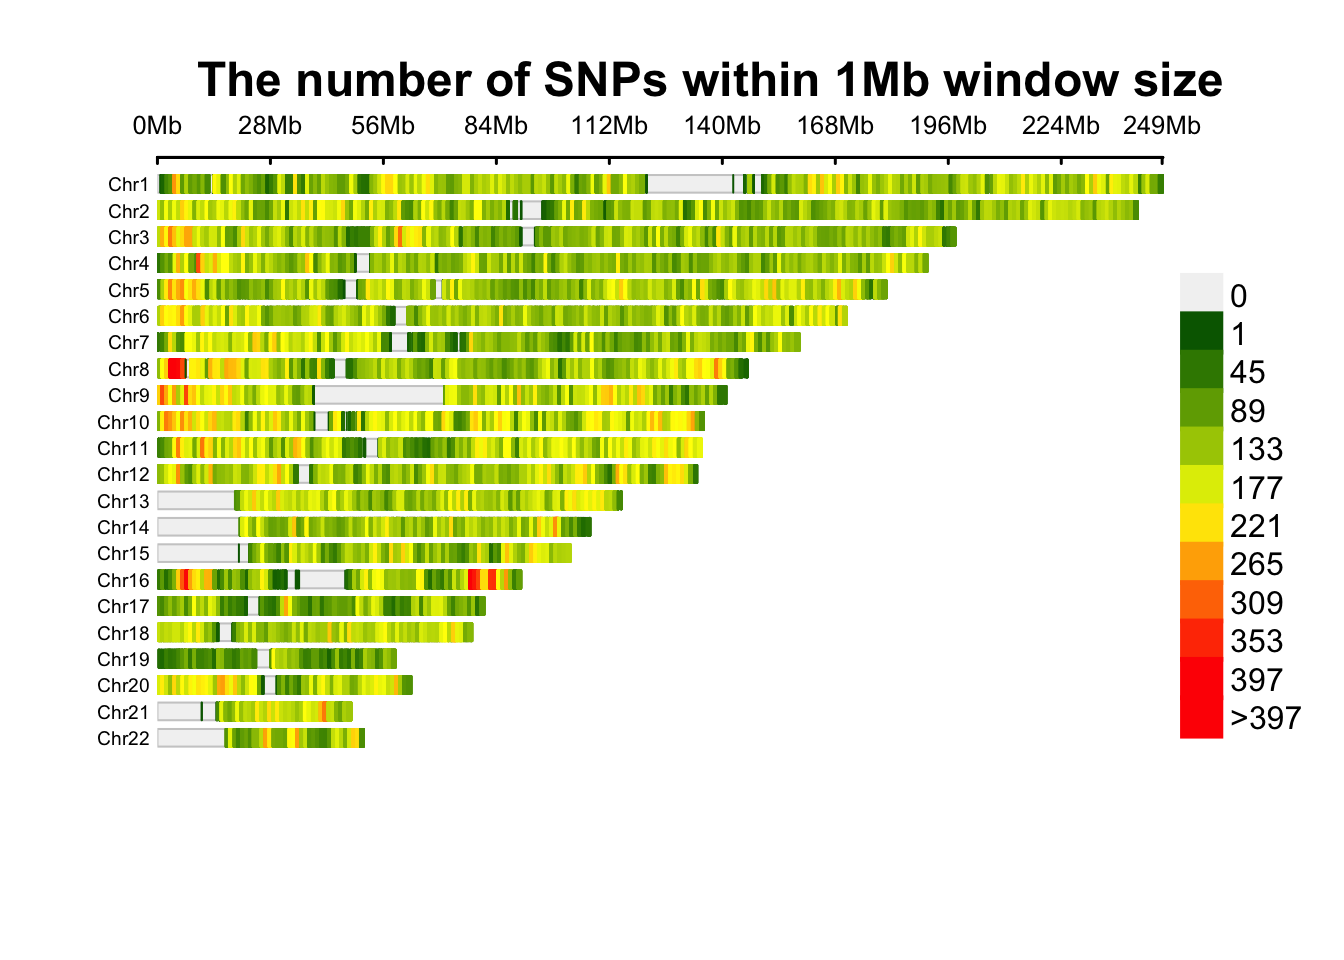
\includegraphics[width=0.85\linewidth]{img/_gwas_wtccc/WTCCC1ResultsManhattan-density} 

}

\caption{SNP density of the association results.}\label{fig:show-wtccc1-graphs-density}
\end{figure}

\begin{figure}[H]

{\centering 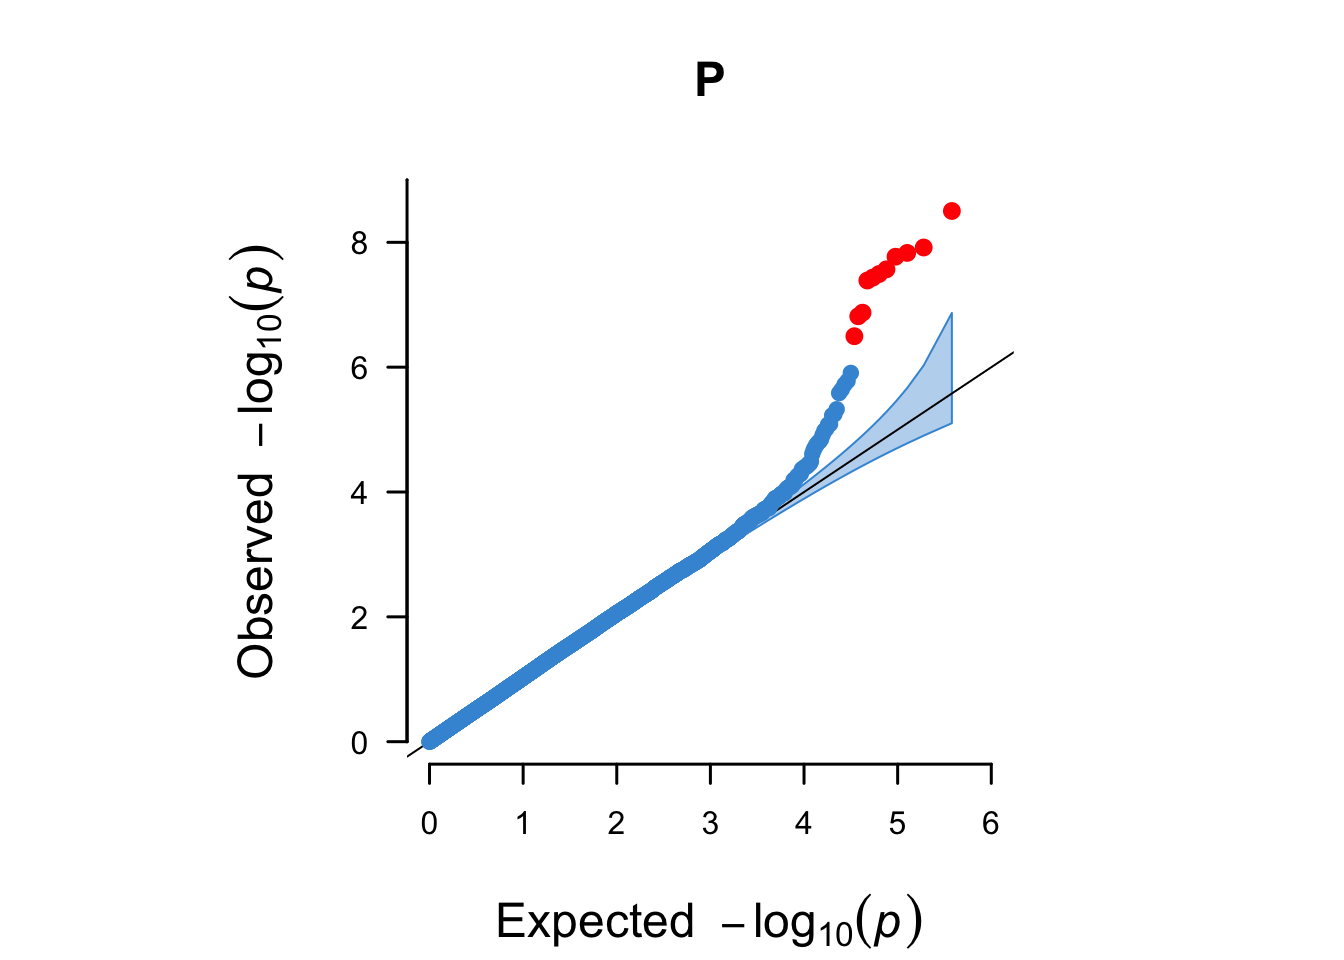
\includegraphics[width=0.85\linewidth]{img/_gwas_wtccc/WTCCC1ResultsManhattan-qq} 

}

\caption{A QQ plot including a 95\% confidence interval (blue area) and genome-wide significant hits (red).}\label{fig:show-wtccc1-graphs-qq}
\end{figure}

\begin{figure}[H]

{\centering 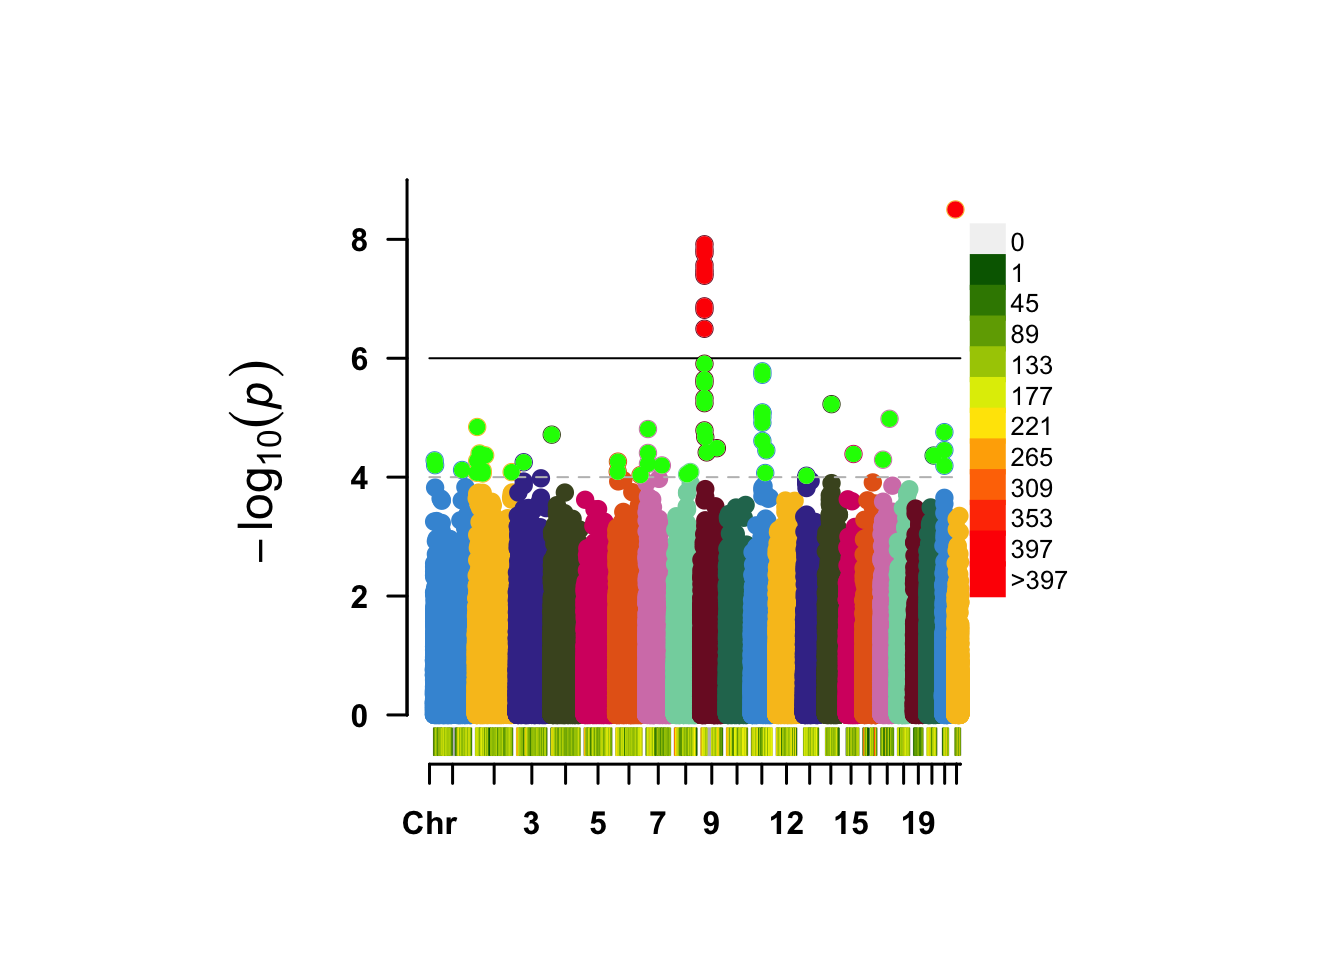
\includegraphics[width=0.85\linewidth]{img/_gwas_wtccc/WTCCC1ResultsManhattan-manhattan} 

}

\caption{A regular manhattan plot. Colored by chromosome, suggestive hits are green, genome-wide hits are red. The bottom graph shows the per-chromosome SNP density.}\label{fig:show-wtccc1-graphs-manhattan}
\end{figure}

\begin{figure}[H]

{\centering 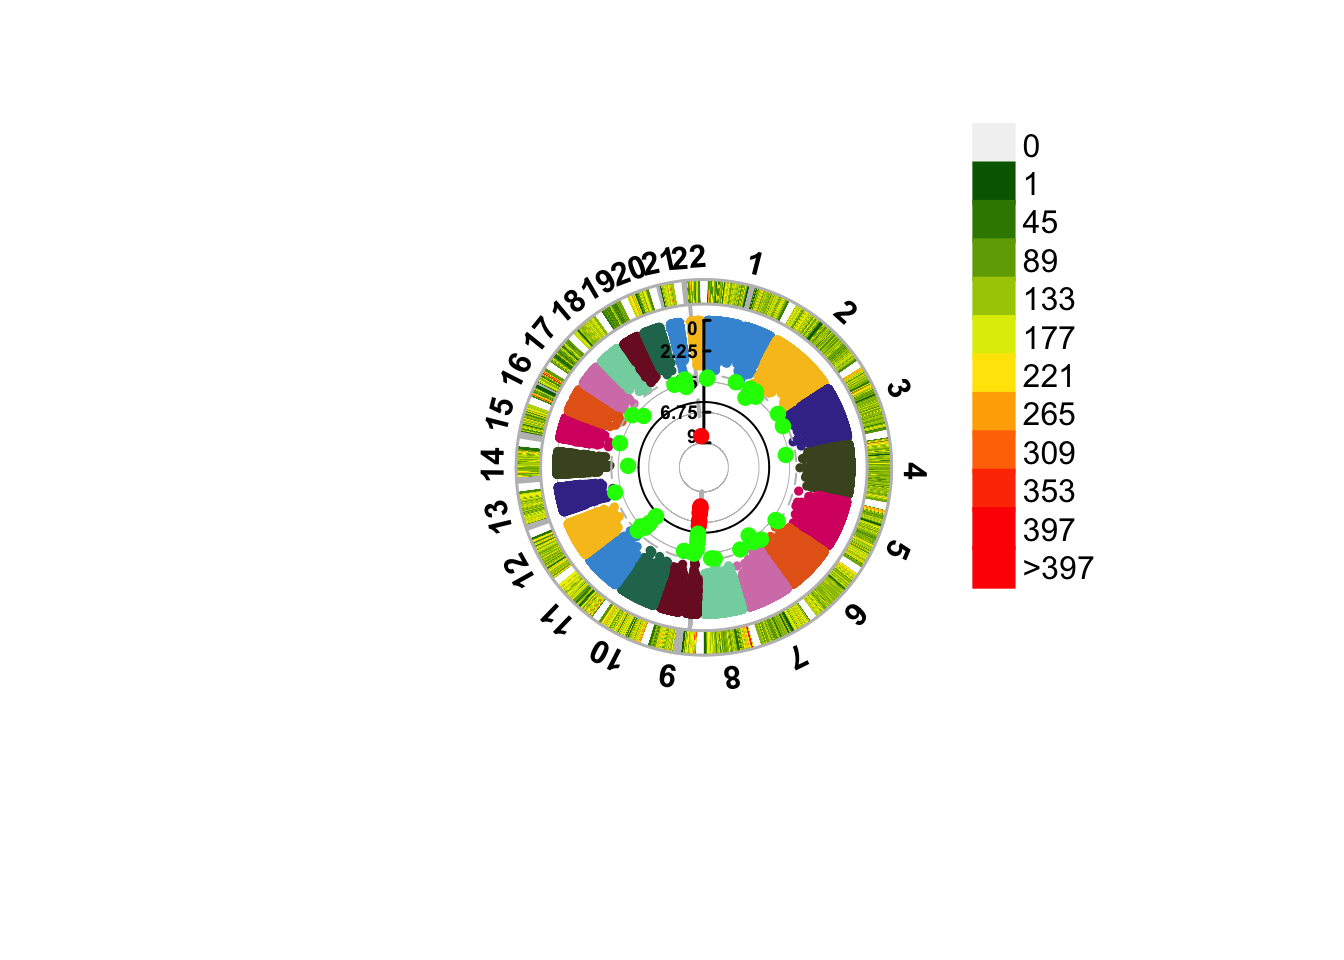
\includegraphics[width=0.85\linewidth]{img/_gwas_wtccc/WTCCC1ResultsManhattan-circular} 

}

\caption{A circular manhattan.}\label{fig:show-wtccc1-graphs-circular}
\end{figure}

\hypertarget{replication}{%
\section{Replication!}\label{replication}}

You reached an important milestone.

\textbf{You recreated the work by the whole WTCCC1-team that took them years in just one afternoon!}

Wow. Take a pause. And realize what you've done.

Back then there wasn't much on analyses \emph{after} a GWAS, nowadays there are many post-GWAS analyses methods. We will cover them in the next Chapter @ref(post\_gwas).

\hypertarget{post_gwas}{%
\chapter{Post-GWAS Analyses}\label{post_gwas}}

A critical step in post-GWAS analysis is probably `mapping SNPs to genes'. It is critical, but it is also the most challenging. \emph{How do you even map SNPs to genes?} What criteria to use? Should we take into account physical position? Or is it of interest that certain SNPs might influence downstream or upstream gene expression? And what of the fact that most loci discovered in GWAS are \_inter\_genic? What is the heritability of our trait? Are there any pleiotropic effects?

In the next few sections I deal with a couple of the downstream, post-GWAS analyses. We don't have time to go practically into a few of these steps, but I do believe it is important to provide you with some pointers where to start.

\hypertarget{clumping}{%
\section{Clumping}\label{clumping}}

The Manhattan plot immediately draws your attention to the peaks above the genome-wide significance threshold. \textbf{Clumping} is the procedure in which we identify the \emph{independent hits}, those top variants and the variants in linkage disequilibrium (their `LD buddies') in the same genomic region (\emph{locus}). The basic steps are as follows. First define a threshold above which to identify the top variant, usually this is the genome-wide significance threshold. Next, define the maximum p-value of association a variant may have with the trait of interest. Define the strength of the correlation that is allowed between the top variant and its LD buddies. And lastly define the size of region around the top variant to assess.

\textbf{Clumping} can easily be done in PLINK. And you can too with the dummy GWAS dataset in this additional chapter @ref(add\_chapter\_regional\_plot). You don't have to now, it's just for fun.

\hypertarget{conditional-analyses}{%
\section{Conditional analyses}\label{conditional-analyses}}

The visualization of a GWAS is very appealing and draws attention to single peaks, and the most significant variant. And with \textbf{clumping} you can identify the independent signals, \emph{i.e.} the top variants and their LD buddies in the locus. We implicitly assume that the top variant captures all the variation in the region by its linkage disequilibrium with an unknown causal variant, in other words it is `tagging' the (un)measured potential causal variant in the region. Intuitively it is unlikely that a single causal variant is accounting for all the LD between the unknown causal variant and the measured (genotyped or imputed) variants at the locus. So, a naive focus on only the top variant ignores the fact that multiple causal variants exist and thus the variation captured by that single top variant underestimates the total variation that could be explained by that single region (locus).

\textbf{Conditional analysis} is a tool to identify the secondary variants associated with the trait of interest. This involves conditioning the association model (\passthrough{\lstinline!trait \~ Variant X + covariates!}) on the primary variant associated in that locus. A more comprehensive and general approach would be to condition on each variant in the whole genome starting with the top variants and stepwise selecting additional variants according to their conditional p-values. This strategy could potentially result in multiple top variants in the same locus. In other words, it could uncover different haplotypes that are causing the same association with the trait of interest.

This would be straightforward with super computers and full-access to individual level data. Unfortunately we often have neither.

Don't despair, a method exists that fills this gap. With the program \href{http://cnsgenomics.com/software/gcta/\#Overview}{GCTA} you can execute conditional analyses on GWAS summary statistics - the kind you just produced with the dummy data and with the WTCCC1 dataset - and a proper reference. You can read more on this in \href{https://www.nature.com/articles/ng.2213}{the paper}.

For now, we will skip this part. I will add a whole chapter on this at some later stage.

\hypertarget{statistical-finemapping}{%
\section{Statistical finemapping}\label{statistical-finemapping}}

\textbf{Statistical finemapping} is closely related to \textbf{conditional analysis}. Where \textbf{conditional analysis} identifies secondary signals in a region associated to the trait of interest, \textbf{statistical finemapping} answers the question `which variants are likely causal to the trait?'. In more formal words, through \textbf{statistical finemapping} we identify the \emph{95\% credible set of causal variants}.
There are multiple methods and tools developed to get to this answer. I list a few and I encourage you to read up on these.

\textbf{FINEMAP}

This tool is very fast and versatile, and was developed by Christian Benner. It will identify the \emph{credible sets} for each locus and calculates the \emph{posterior probabilities} for each set. This is the more hands-on version of getting to \emph{credible sets}.

\textbf{LocusZoom}

You could upload - privately or publicly - your data to \href{https://my.locuszoom.org}{my.locuszoom.org} and obtain a list of causal variants with posterior probabilities. It uses a \href{https://statgen.github.io/gwas-credible-sets/method/locuszoom-credible-sets.pdf}{simple procedure} to obtain the \emph{credible sets} using \href{https://github.com/statgen/gwas-credible-sets/}{these scripts}. This is the more lazy version of getting a list of likely causal variants.

\textbf{SuSIE}

An laternate approach to \emph{credible set} identification is through \href{https://stephenslab.github.io/susieR/index.html}{SuSIE}. Through SuSIE you can identify \emph{credible sets} under the assumption of multiple causal variants, whereas \textbf{FINEMAP} assumes a single causal variant.

For now, we will skip this part. I will add a whole chapter on this at some later stage.

\hypertarget{fuma-functional-mapping-and-annotation-of-gwas}{%
\section{FUMA: FUnctional Mapping and Annotation of GWAS}\label{fuma-functional-mapping-and-annotation-of-gwas}}

Researchers from the VUMC in Amsterdam have created an online tool that aids in mapping genes and function to GWAS: \emph{``Functional Mapping and Annotation of Genome-Wide Association Studies''} a.k.a. \href{https://fuma.ctglab.nl}{FUMA}. This online tool uses a variety of datasets and programs to prioritize genes and map these to associated loci.

We have covered some aspects of post-GWAS analyses, and a lot are covered by FUMA. Let's try and annotate our WTCCC1 results. The assignment in this chapter \ref{fuma} will be a bit more \emph{Do It Yourself}.

\hypertarget{phenome-wide-association-study}{%
\section{Phenome-wide association study}\label{phenome-wide-association-study}}

A \textbf{phenome-wide association study}, or \textbf{PheWAS}, deals with assessing the association of top variants identified in GWAS with other traits. Through a \textbf{PheWAS} you'll to get a notion whether on any of the top variants, the independent hits in your GWAS, have pleiotropic effects. In other words, whether your independent hits have effects on other traits too. This will paint a picture as it were about the role the genetic locus you identified plays in life: is it unique to your trait or does it affect other traits as well? What does it mean when your top variant near the gene \emph{FTO} associates not only to BMI, but also to type 2 diabetes and coronary artery disease? \textbf{PheWAS} will not answer that question, but they do help in inventory all the other traits to which your hits are associated.

Again, we'll get a bit hands-on and more \emph{Do It Yourself} in the chapter that deals with this. Let's jump over to Chapter \ref{phewas}.

\hypertarget{colocalization}{%
\section{Colocalization}\label{colocalization}}

From all of the above follows another intuitive question. Suppose a signal in your trait also shows association - to some extent - with other traits. Do these two signals than significantly overlap, more so than you would think based on chance? \textbf{Colocalization} deals with exactly this question.

We are not going to deal with \textbf{colocalization}, but a nice starting point is \href{https://github.com/oliviasabik/RACER}{RACER} about which you can read more in chapter @ref(add\_chapter\_regional\_plot). I will add a whole chapter on this at some later stage.

\hypertarget{genetic-correlation}{%
\section{Genetic correlation}\label{genetic-correlation}}

Because of the underlying biology or because of the way they are measured or calculated, traits can be highly correlated - phenotypically. That is to say, when the levels of HDL are high, LDL is probably low, and so when you draw a correlation plot from some data obtained in a general population you'll see a nice pattern. Biology may also cause traits to be genetically correlated: the same genetic variants influence multiple traits. In other words, if a variant is associated with higher levels of LDL-cholesterol, it may alternatively be associated with lower HDL-cholesterol, etc. Genetic correlation will aid in further understanding the relations between traits biologically: if there is a strong \textbf{genetic correlation}, it is may be due to the same biological pathways and so the traits are `linked' through the same processes (maybe counter-acting processes).

\begin{quote}
Puzzle: what other phenomenom could cause a high but spurious \textbf{genetic correlation}?
\end{quote}

We are not going to deal with \textbf{genetic correlation}. I will add a whole chapter on this at some later stage.

\hypertarget{causal-inference-mendelian-randomization}{%
\section{Causal inference: Mendelian Randomization}\label{causal-inference-mendelian-randomization}}

In observational studies we may find a strong association between a certain risk factor or biomarker and a disease. For instance, epidemiological studies show that high circulating cystatin C is associated with risk of cardiovascular disease (CVD), independent of creatinine-based renal function measurements\citep{vanderlaan2016}. However, residual confounding and reverse causality remain alternative explanations for the strong correlation between cystatin C and CVD, both of which are difficult to tease apart from traditional observational (epidemiological) studies.

\textbf{Mendelian Randomization (MR)} harnesses the properties of the genome to enable causal inference of a biomarker. Specifically, the invariant nature of the genome and the random distribution of alleles from parents to offspring at conception mean that genetic information is not influenced by disease status (reverse causality) and should be free from confounding by traditional risk factors\citep{vanderlaan2016}. So, genetic variation that modulates serum concentrations of cystatin C could serve as an instrumental variable to assess the effect of lifelong elevated concentrations of cystatin C on disease risk, independent of potential confounders\citep{vanderlaan2016}.

Finding the causal genes for complex disease is a primary objective of many researchers, because these genes are putative therapeutic targets. In this course we intend to find out whether Type 2 Diabetes (T2D) causes coronary artery disease and ischemic stroke.

There is an easy, quick-and-dirty way and a harder way.

\textbf{MRBase}

The quick-and-dirty way uses \href{http://www.mrbase.org/}{MRBase}. It is based on the \passthrough{\lstinline!TwoSampleMR!} package and uses the \passthrough{\lstinline!MRInstruments!} package to load in all the genetic instruments. The creators of MRBase have curated hundreds of GWAS and molecular QTL studies, and prepared the data for easy use on the website and in the R packages.

\textbf{TwoSampleMR}

The hard way means getting your hands dirty and using the \passthrough{\lstinline!TwoSampleMR!} package yourself in \passthrough{\lstinline!R!}. You'll learn all the steps you need to take into account to get to the answer of this question. You'll create the diagnostic graphs and calculate the statistics.

\hypertarget{your-choice}{%
\subsection{Your choice}\label{your-choice}}

Your choice. In both cases you'll learn how to do execute a MR, what to look out for in the statistics and diagnostic graphs, and how interpret the results. Your choice: Chapter @ref(mr\_mrbase) or Chapter @ref(mr\_twosamplemr).

In a future version I will aim to include a partial replication of the Cystatin C paper\citep{vanderlaan2016}

\hypertarget{polygenic-scores}{%
\section{Polygenic scores}\label{polygenic-scores}}

Under the assumption of polygenicity, many variants with small effects contribute to the phenotypic variation in a trait or the risk to disease. Sample size and accurate phenotyping have a major impact on the power of a GWAS. It is estimated that 70\% of variants that reach 10-6 in an initial discovery GWAS will reach genome-wide significance with increasing sample sizes. The individual variants that do reach genome-wide significance the first or second time around do not explain \emph{all} the phenotypic variation or residual disease risk.

To capture the polygenicity of a trait beyond individual genome-wide significant hits, we can calculate a polygenic score (PGS). There are several methods to calculate PGS, but essentially it comes down to multiplying the effect size at a given variant with the number of effect alleles a given individual carries.
Depending on the method you can use the `hard-coded' genotyped data, or the imputed data. In case of the latter the effect sizes are multiplied by the genotype probabilities or dosages, this ensures that the PGS takes into account the uncertainty intrinsic to imputed data.

Let's consider the most intuitive PGS-method which is based on p-value thresholding, which was nicely applied in this classic \href{https://doi.org/10.1038/nature08185}{paper}. This method selects variants based on their p-value and than calculates the PGS. This can be done using increasingly liberal significance thresholds (pT), for instance starting with all variants with p \textless{} 10-8, next p \textless{} 10-7, p \textless{} 10-6, p \textless{} 10-5, p \textless{} 10-4, p \textless{} 10-3, p \textless{} 0.05, p \textless{} 0.1, p \textless{} 0.2, p \textless{} 0.3, p \textless{} 0.4, p \textless{} 0.5. Under the assumption of polygenicity we expect an increasingly stronger correlation (r2) of the PGS at a certain pT with the trait of interest. Another application of this method is provided by Van Setten\citep{vansetten2015}.

Lastly, there is a great explanatory \href{http://polygenicscores.org/explained/}{website} on how to calculate PGS, and it also shows one application of PGS (although much debate ensues about this particular application!).

\hypertarget{what-comes-next}{%
\section{What comes next}\label{what-comes-next}}

You come to the end of this practical primer. What is left are a summary (not written yet) of what you've learned and should take home. And some musings in the Epilogue (\ref{epilogue} on this book and what the future holds.

\hypertarget{conditional_analysis}{%
\chapter{Conditional analysis}\label{conditional_analysis}}

\hypertarget{section-1}{%
\section{Section 1}\label{section-1}}

Lorem ipsum dolor sit amet, consectetur adipiscing elit, sed do eiusmod tempor incididunt ut labore et dolore magna aliqua. Ut enim ad minim veniam, quis nostrud exercitation ullamco laboris nisi ut aliquip ex ea commodo consequat. Duis aute irure dolor in reprehenderit in voluptate velit esse cillum dolore eu fugiat nulla pariatur. Excepteur sint occaecat cupidatat non proident, sunt in culpa qui officia deserunt mollit anim id est laborum.

\hypertarget{section-2}{%
\section{Section 2}\label{section-2}}

Sed ut perspiciatis unde omnis iste natus error sit voluptatem accusantium doloremque laudantium, totam rem aperiam, eaque ipsa quae ab illo inventore veritatis et quasi architecto beatae vitae dicta sunt explicabo. Nemo enim ipsam voluptatem quia voluptas sit aspernatur aut odit aut fugit, sed quia consequuntur magni dolores eos qui ratione voluptatem sequi nesciunt. Neque porro quisquam est, qui dolorem ipsum quia dolor sit amet, consectetur, adipisci velit, sed quia non numquam eius modi tempora incidunt ut labore et dolore magnam aliquam quaerat voluptatem. Ut enim ad minima veniam, quis nostrum exercitationem ullam corporis suscipit laboriosam, nisi ut aliquid ex ea commodi consequatur? Quis autem vel eum iure reprehenderit qui in ea voluptate velit esse quam nihil molestiae consequatur, vel illum qui dolorem eum fugiat quo voluptas nulla pariatur?

\hypertarget{section-3}{%
\section{Section 3}\label{section-3}}

At vero eos et accusamus et iusto odio dignissimos ducimus qui blanditiis praesentium voluptatum deleniti atque corrupti quos dolores et quas molestias excepturi sint occaecati cupiditate non provident, similique sunt in culpa qui officia deserunt mollitia animi, id est laborum et dolorum fuga. Et harum quidem rerum facilis est et expedita distinctio. Nam libero tempore, cum soluta nobis est eligendi optio cumque nihil impedit quo minus id quod maxime placeat facere possimus, omnis voluptas assumenda est, omnis dolor repellendus. Temporibus autem quibusdam et aut officiis debitis aut rerum necessitatibus saepe eveniet ut et voluptates repudiandae sint et molestiae non recusandae. Itaque earum rerum hic tenetur a sapiente delectus, ut aut reiciendis voluptatibus maiores alias consequatur aut perferendis doloribus asperiores repellat.

\hypertarget{replication-1}{%
\section{Replication!}\label{replication-1}}

You reached an important milestone: you recreated the work by the whole WTCCC1 in just an afternoon. Wow. Back then there wasn't much on analyses \emph{after} a GWAS, nowadays there are many post-GWAS analyses methods. We will cover them in the next Chapter \ref{finemapping}.

\hypertarget{finemapping}{%
\chapter{Statistical finemapping}\label{finemapping}}

\hypertarget{section-1-1}{%
\section{Section 1}\label{section-1-1}}

Lorem ipsum dolor sit amet, consectetur adipiscing elit, sed do eiusmod tempor incididunt ut labore et dolore magna aliqua. Ut enim ad minim veniam, quis nostrud exercitation ullamco laboris nisi ut aliquip ex ea commodo consequat. Duis aute irure dolor in reprehenderit in voluptate velit esse cillum dolore eu fugiat nulla pariatur. Excepteur sint occaecat cupidatat non proident, sunt in culpa qui officia deserunt mollit anim id est laborum.

\hypertarget{section-2-1}{%
\section{Section 2}\label{section-2-1}}

Sed ut perspiciatis unde omnis iste natus error sit voluptatem accusantium doloremque laudantium, totam rem aperiam, eaque ipsa quae ab illo inventore veritatis et quasi architecto beatae vitae dicta sunt explicabo. Nemo enim ipsam voluptatem quia voluptas sit aspernatur aut odit aut fugit, sed quia consequuntur magni dolores eos qui ratione voluptatem sequi nesciunt. Neque porro quisquam est, qui dolorem ipsum quia dolor sit amet, consectetur, adipisci velit, sed quia non numquam eius modi tempora incidunt ut labore et dolore magnam aliquam quaerat voluptatem. Ut enim ad minima veniam, quis nostrum exercitationem ullam corporis suscipit laboriosam, nisi ut aliquid ex ea commodi consequatur? Quis autem vel eum iure reprehenderit qui in ea voluptate velit esse quam nihil molestiae consequatur, vel illum qui dolorem eum fugiat quo voluptas nulla pariatur?

\hypertarget{section-3-1}{%
\section{Section 3}\label{section-3-1}}

At vero eos et accusamus et iusto odio dignissimos ducimus qui blanditiis praesentium voluptatum deleniti atque corrupti quos dolores et quas molestias excepturi sint occaecati cupiditate non provident, similique sunt in culpa qui officia deserunt mollitia animi, id est laborum et dolorum fuga. Et harum quidem rerum facilis est et expedita distinctio. Nam libero tempore, cum soluta nobis est eligendi optio cumque nihil impedit quo minus id quod maxime placeat facere possimus, omnis voluptas assumenda est, omnis dolor repellendus. Temporibus autem quibusdam et aut officiis debitis aut rerum necessitatibus saepe eveniet ut et voluptates repudiandae sint et molestiae non recusandae. Itaque earum rerum hic tenetur a sapiente delectus, ut aut reiciendis voluptatibus maiores alias consequatur aut perferendis doloribus asperiores repellat.

\hypertarget{replication-2}{%
\section{Replication!}\label{replication-2}}

You reached an important milestone: you recreated the work by the whole WTCCC1 in just an afternoon. Wow. Back then there wasn't much on analyses \emph{after} a GWAS, nowadays there are many post-GWAS analyses methods. We will cover them in the next Chapter \ref{fuma}.

\hypertarget{fuma}{%
\chapter{Functional Mapping and Annotation of GWAS}\label{fuma}}

\hypertarget{assignment-1}{%
\section{Assignment}\label{assignment-1}}

\hypertarget{tutorial}{%
\subsection{Tutorial}\label{tutorial}}

Go to the \href{https://fuma.ctglab.nl}{FUMA website}, get an account, and study the \href{https://fuma.ctglab.nl/tutorial}{online-tutorial}.

\hypertarget{create-the-input}{%
\subsection{Create the input}\label{create-the-input}}

You will need to use the \passthrough{\lstinline!fwrite!} function in \passthrough{\lstinline!r!} to write the concatenated results of the WTCCC1 study (remember: \passthrough{\lstinline!wtccc1\_assoc\_compl!}).

\begin{quote}
Question: can you figure out the sample size of the WTCCC1 data you used?
\end{quote}

Make sure you know what the column-names are in the file, you'll need that for FUMA. You can use \passthrough{\lstinline!cat your\_file | head!} to get the first 10 lines of the file.

You will need to compress the resulting output, this will make uploading to FUMA go faster. You can use the \passthrough{\lstinline!bash!}-program \passthrough{\lstinline!gzip!} for that. If you want to know what the options are for that program, you can use \passthrough{\lstinline!gzip -h!}.

\hypertarget{run-fuma---snp-to-gene}{%
\subsection{Run FUMA - SNP to gene}\label{run-fuma---snp-to-gene}}

Upload via the form on the FUMA-website. Since you've done the tutorial you are familiar with its options.

Select \emph{everything} in the tabs \passthrough{\lstinline!Gene Mapping (positional mapping)!}, \passthrough{\lstinline!Gene Mapping (eQTL mapping)!} but \emph{not} \passthrough{\lstinline!GTEx v6!} and \passthrough{\lstinline!GTEx v7!}, and \passthrough{\lstinline!Gene Mapping (3D Chromatin Interaction mapping)!} and leave the settings at \passthrough{\lstinline!Gene types!} and \passthrough{\lstinline!MHC region!} as-is. At \passthrough{\lstinline!MAGMA analysis!} set the \emph{MAGMA gene expression analysis} to include all tissues, \emph{but} \passthrough{\lstinline!GTEx v6!} and \passthrough{\lstinline!GTEx v7!}.

Don't forget to give your analysis a name.

This will take some time and so it's a good moment to carry on with the rest of the practical or take a break, or study for the exam.

\begin{quote}
Questions

\begin{enumerate}
\def\labelenumi{\arabic{enumi}.}
\tightlist
\item
  How many lead SNPs did we find?
\item
  What do the results of MAGMA (the gene-based test) look like and how many genes pass the threshold of multiple testing correction?
\item
  How many loci were mapped?
\item
  How many genes were physically located and how many were mapped to these loci?
\item
  Do you think all loci are `correct', \emph{i.e.} do you `believe' all the signals looking at the mapping results? Why?
\item
  For what tissues are the signals enriched?
\item
  Are there any chromatin interactions discovered?
\end{enumerate}
\end{quote}

\hypertarget{run-fuma---gene-to-function}{%
\subsection{Run FUMA - Gene to function}\label{run-fuma---gene-to-function}}

Now that you mapped SNPs to genes, it's time to go back to `My Jobs'. Select your job and perform \passthrough{\lstinline!GENE2FUNC!}.

\begin{quote}
Questions

\begin{enumerate}
\def\labelenumi{\arabic{enumi}.}
\tightlist
\item
  What genes show the lowest expression across tissues?
\item
  And what genes the highest?
\item
  For what pathways are the signals enriched?
\item
  What molecular functions are mapped to the signals?
\end{enumerate}
\end{quote}

\hypertarget{some-closing-thoughts}{%
\section{Some closing thoughts}\label{some-closing-thoughts}}

FUMA is a great tool, but it comes with a caveat. It includes a couple of references of which it is not readily clear which variants are included - the authors do provide the codes used on Git, but still, you don't know which variants precisely are filtered. That is key: perhaps the top variant you discovered is filtered in the reference. This means FUMA will not use it to map SNPs to genes, rather next best variant. This should be in high-LD - but, again, assumptions\ldots{} And of course, the references used might not match your data well enough.
So, my advice: use FUMA (why not be lazy rather than work hard?), but aware of such caveats as I described. All in all, I do think FUMA is very complete, intuitive, and it makes your work publication-ready because it creates just the right file-formats for you too (\passthrough{\lstinline!.png!}, \passthrough{\lstinline!.svg!}, \passthrough{\lstinline!.pdf!}, \passthrough{\lstinline!.jpeg!}).

That said, time to move on to inspect other phenotypes in relation to your findings in the next Chapter \ref{phewas} or to return to the previous chapter on post-GWAS analyses @ref(post\_gwas).

\hypertarget{phewas}{%
\chapter{Phenome-Wide Association Study}\label{phewas}}

Given the large biobanks available nowadays that have also genotyped the participants and collected a vast-array of information on them, it is possible to perform a \textbf{Phe}nome-\textbf{W}ide \textbf{A}ssociation \textbf{S}tudy.

There are several options in (Table \ref{tab:tab-phewas}).

\begin{table}

\caption{\label{tab:tab-phewas}PheWAS Resources.}
\centering
\begin{tabular}[t]{l|l}
\hline
Site & Description\\
\hline
https://atlas.ctglab.nl & 4,155 GWAS based on UK Biobank release 2\\
\hline
https://biobankengine.stanford.edu & UK Biobank based\\
\hline
http://pheweb.sph.umich.edu & University of Michigan EHR-based PheWAS\\
\hline
http://pheweb.sph.umich.edu/SAIGE-UKB/ & 1,403 GWAS UK Biobank based\\
\hline
http://phewas.mrbase.org & UK Biobank based\\
\hline
\end{tabular}
\end{table}

\emph{Assignment}

\begin{enumerate}
\def\labelenumi{\arabic{enumi}.}
\tightlist
\item
  Perform a PheWAS with a few of the resources and your favorite SNP from this tutorial.
\item
  Compare the different websites. What do you notice?
\item
  How is a PheWAS informative?
\end{enumerate}

\hypertarget{whats-next}{%
\section{What's next?}\label{whats-next}}

You now know to what other traits, risk factors and diseases our trait of interest (coronary artery disease) is correlated. An obvious next question would be: is this a causal correlation? We will cover this aspect in the next Chapter @ref(mendelian\_randomization) or to return to the previous chapter on post-GWAS analyses @ref(post\_gwas).

\hypertarget{mr_mrbase}{%
\chapter{MRBase}\label{mr_mrbase}}

You took the easy way out. No shame in that. Your choice. Right, so as I wrote, \emph{\href{http://www.mrbase.org/}{MRBase}} is very easy to handle. It is based on the \passthrough{\lstinline!TwoSampleMR!} package and uses the \passthrough{\lstinline!MRInstruments!} package to load in all the genetic instruments. The creators of MRBase have curated hundreds of GWAS and molecular QTL studies, and prepared the data for easy use on the website and in the R packages.

Using \textbf{\href{http://www.mrbase.org/}{MRBase}} we intend to find out whether Type 2 Diabetes (T2D) causes coronary artery disease and ischemic stroke.

\hypertarget{the-end}{%
\section{The end?}\label{the-end}}

You are almost at the end. Time to return to the previous chapter on post-GWAS analyses @ref(post\_gwas).

\hypertarget{summary}{%
\chapter*{Summary}\label{summary}}
\addcontentsline{toc}{chapter}{Summary}

\hypertarget{section-1-2}{%
\section{Section 1}\label{section-1-2}}

Lorem ipsum dolor sit amet, consectetur adipiscing elit, sed do eiusmod tempor incididunt ut labore et dolore magna aliqua. Ut enim ad minim veniam, quis nostrud exercitation ullamco laboris nisi ut aliquip ex ea commodo consequat. Duis aute irure dolor in reprehenderit in voluptate velit esse cillum dolore eu fugiat nulla pariatur. Excepteur sint occaecat cupidatat non proident, sunt in culpa qui officia deserunt mollit anim id est laborum.

\hypertarget{section-2-2}{%
\section{Section 2}\label{section-2-2}}

Sed ut perspiciatis unde omnis iste natus error sit voluptatem accusantium doloremque laudantium, totam rem aperiam, eaque ipsa quae ab illo inventore veritatis et quasi architecto beatae vitae dicta sunt explicabo. Nemo enim ipsam voluptatem quia voluptas sit aspernatur aut odit aut fugit, sed quia consequuntur magni dolores eos qui ratione voluptatem sequi nesciunt. Neque porro quisquam est, qui dolorem ipsum quia dolor sit amet, consectetur, adipisci velit, sed quia non numquam eius modi tempora incidunt ut labore et dolore magnam aliquam quaerat voluptatem. Ut enim ad minima veniam, quis nostrum exercitationem ullam corporis suscipit laboriosam, nisi ut aliquid ex ea commodi consequatur? Quis autem vel eum iure reprehenderit qui in ea voluptate velit esse quam nihil molestiae consequatur, vel illum qui dolorem eum fugiat quo voluptas nulla pariatur?

\hypertarget{section-3-2}{%
\section{Section 3}\label{section-3-2}}

At vero eos et accusamus et iusto odio dignissimos ducimus qui blanditiis praesentium voluptatum deleniti atque corrupti quos dolores et quas molestias excepturi sint occaecati cupiditate non provident, similique sunt in culpa qui officia deserunt mollitia animi, id est laborum et dolorum fuga. Et harum quidem rerum facilis est et expedita distinctio. Nam libero tempore, cum soluta nobis est eligendi optio cumque nihil impedit quo minus id quod maxime placeat facere possimus, omnis voluptas assumenda est, omnis dolor repellendus. Temporibus autem quibusdam et aut officiis debitis aut rerum necessitatibus saepe eveniet ut et voluptates repudiandae sint et molestiae non recusandae. Itaque earum rerum hic tenetur a sapiente delectus, ut aut reiciendis voluptatibus maiores alias consequatur aut perferendis doloribus asperiores repellat.

\hypertarget{replication-3}{%
\section{Replication!}\label{replication-3}}

You reached an important milestone: you recreated the work by the whole WTCCC1 in just an afternoon. Wow. Back then there wasn't much on analyses \emph{after} a GWAS, nowadays there are many post-GWAS analyses methods. We will cover them in the next (Chapter \ref{epilogue}).

\hypertarget{epilogue}{%
\chapter{Epilogue}\label{epilogue}}

What started as a simple `let's write a practical on how to do a GWAS', escalated into this GitBook. My second book. My fifth child (as far as I know). I hope you found it to be useful and learned a bit.

That said, much can be improved and so don't hesitate to contact me.

As with any proper epilogue I should not forget a heartfelt and honest thank you to the readers and users of this work. Gratitude also goes to my dear colleagues Charlotte Onland, Jessica van Setten, and Kristel van Eijk, and former colleague Sara Pulit who asked me back in 2017 to join the course as a lecturer. It has been a pleasure to work with and learn from you, and it has been a fun (and sometimes stressful) experience to teach this course.

\hypertarget{eigensoft}{%
\chapter{Additional: EIGENSOFT}\label{eigensoft}}

There used to be a time that the preferred software \textbf{\href{https://github.com/DReichLab/EIG}{\passthrough{\lstinline!EIGENSOFT!}}} for Principal Component Analysis (PCA) was \textbf{\passthrough{\lstinline!EIGENSOFT!}} For many, it still is. However, \textbf{\passthrough{\lstinline!EIGENSOFT!}} is a bit challenging to make it work to say the least. You need to install some programs, and this is not always straightforward.

So, here's the deal.

I will share the how-to for a macOS environment below in {[}EIGENSOFT{]} - this should work in a Linux environment too as macOS is UNIX-based. You can choose to try and make it work on your system (be it UNIX or macOS based) at home (or in the office).

However, I recommend that you use the \passthrough{\lstinline!--pca!} function which is present in \passthrough{\lstinline!PLINK!} v1.9 and up. This means you should probably simply skip this section and jump straight to Chapter \ref{gwas-basics-sample-qc}.

\hypertarget{install-homebrew}{%
\section{Install homebrew}\label{install-homebrew}}

You need to install \passthrough{\lstinline!brew!}, the missing package-manager and accompanying packages that Apple didn't provide.

\begin{lstlisting}
/bin/bash -c "$(curl -fsSL https://raw.githubusercontent.com/Homebrew/install/HEAD/install.sh)"
\end{lstlisting}

Next, check that everything is in order.

\begin{lstlisting}
brew doctor
\end{lstlisting}

\hypertarget{install-missing-packages}{%
\section{Install missing packages}\label{install-missing-packages}}

Right, now that you've done that, you're ready to install \passthrough{\lstinline!gsl!} and \passthrough{\lstinline!openblas!}.

\begin{lstlisting}
brew install gsl
brew install openblas
\end{lstlisting}

You may also require \passthrough{\lstinline!llvm!} for \textbf{\passthrough{\lstinline!EIGENSOFT!}} to work.

\begin{lstlisting}
brew install llvm
\end{lstlisting}

\hypertarget{installing-eigensoft}{%
\section{Installing EIGENSOFT}\label{installing-eigensoft}}

I am still sharing the code you'll need - you could try this on your system.

\begin{lstlisting}
mkdir -v $HOME/git
cd $HOME/git
git clone https://github.com/DReichLab/EIG.git
cd EIG/src
make
make install
\end{lstlisting}

\hypertarget{answers}{%
\chapter{Answers to the questions}\label{answers}}

Throughout the book you encountered questions related to some steps and output that you generated. Here you can review the answers for each of these questions - of course, for some different answers are possible.

\begin{quote}
{[}ANSWERS NEED TO BE WORKED OUT{]}
\end{quote}

\hypertarget{chapter-3.1-gwas-basics}{%
\section{Chapter 3.1: GWAS Basics}\label{chapter-3.1-gwas-basics}}

\begin{quote}
Question: Can you think off what the `11,440 heterozygous haploid genotypes present' represent?
\end{quote}

\begin{quote}
Question: Can you think of other scenarios in which you may want to extend the check on differential missingness beyond a check between cases and controls?
* For instance `genotyping platform', or `hospital of inclusion', if you think this might influence the genotyping experiment technically.
\end{quote}

\hypertarget{chapter-3.4-gwas-basics---association-testing}{%
\section{Chapter 3.4: GWAS Basics - Association testing}\label{chapter-3.4-gwas-basics---association-testing}}

\begin{quote}
Question: Load the data using R. {[}Hint: use and adapt the examples from the previous chapters.{]}
\end{quote}

\begin{lstlisting}
library("data.table")

COURSE_loc = "~/Desktop/practical" # getwd()

gwas_HWE <- data.table::fread(paste0(COURSE_loc, "/dummy_project/gwa.hwe"))
gwas_FRQ <- data.table::fread(paste0(COURSE_loc, "/dummy_project/gwa.frq"))
gwas_IMISS <- data.table::fread(paste0(COURSE_loc, "/dummy_project/gwa.imiss"))
gwas_LMISS <- data.table::fread(paste0(COURSE_loc, "/dummy_project/gwa.lmiss"))
\end{lstlisting}

\begin{quote}
Question: Plot the per-stratum HWE p-values using R. {[}Hint: use and adapt the examples from the previous chapters.{]}
\end{quote}

\begin{lstlisting}
library("ggpubr")

gwas_HWE$logP <- -log10(gwas_HWE$P)

ggpubr::gghistogram(gwas_HWE, x = "logP",
                    add = "mean",
                    add.params = list(color = "#595A5C", linetype = "dashed", size = 1),
                    rug = TRUE,
                    # color = "#1290D9", fill = "#1290D9",
                    color = "TEST", fill = "TEST",
                    palette = "lancet",
                    facet.by = "TEST",
                    bins = 50,
                    xlab = "HWE -log10(P)") +
  ggplot2::geom_vline(xintercept = 5, linetype = "dashed",
                      color = "#E55738", size = 1)
ggplot2::ggsave(paste0(COURSE_loc, "/dummy_project/gwas-hwe.png"),
       plot = last_plot())
\end{lstlisting}

\begin{quote}
Question: Plot the allele frequencies using R. {[}Hint: use and adapt the examples from the previous chapters.{]}
\end{quote}

\begin{lstlisting}
ggpubr::gghistogram(gwas_FRQ, x = "MAF",
                    add = "mean", add.params = list(color = "#595A5C", linetype = "dashed", size = 1),
                    rug = TRUE,
                    color = "#1290D9", fill = "#1290D9",
                    xlab = "minor allele frequency") +
  ggplot2::geom_vline(xintercept = 0.05, linetype = "dashed",
                      color = "#E55738", size = 1)
ggplot2::ggsave(paste0(COURSE_loc, "/dummy_project/gwas-freq.png"),
       plot = last_plot())
\end{lstlisting}

\begin{quote}
Question: Plot the per-sample call rates using R. {[}Hint: use and adapt the examples from the previous chapters.{]}
\end{quote}

\begin{lstlisting}
gwas_IMISS$callrate <- 1 - gwas_IMISS$F_MISS

ggpubr::gghistogram(gwas_IMISS, x = "callrate",
                    add = "mean", add.params = list(color = "#595A5C", linetype = "dashed", size = 1),
                    rug = TRUE, bins = 50,
                    color = "#1290D9", fill = "#1290D9",
                    xlab = "per sample call rate") +
  ggplot2::geom_vline(xintercept = 0.95, linetype = "dashed",
                      color = "#E55738", size = 1)
ggplot2::ggsave(paste0(COURSE_loc, "/dummy_project/gwas-sample-call-rate.png"),
       plot = last_plot())
\end{lstlisting}

\begin{quote}
Question: Plot the per-SNP call rates using R. {[}Hint: use and adapt the examples from the previous chapters.{]}
\end{quote}

\begin{lstlisting}
gwas_LMISS$callrate <- 1 - gwas_LMISS$F_MISS

ggpubr::gghistogram(gwas_LMISS, x = "callrate",
                    add = "mean", add.params = list(color = "#595A5C", linetype = "dashed", size = 1),
                    rug = TRUE, bins = 50,
                    color = "#1290D9", fill = "#1290D9",
                    xlab = "per SNP call rate") +
  ggplot2::geom_vline(xintercept = 0.95, linetype = "dashed",
                      color = "#E55738", size = 1)
ggplot2::ggsave(paste0(COURSE_loc, "/dummy_project/gwas-snp-call-rate.png"),
       plot = last_plot())
\end{lstlisting}

\begin{quote}
Question: Do you know which model, \emph{i.e.} \passthrough{\lstinline!TEST!} is most commonly used and reported? And why is that, do think?
\end{quote}

\begin{quote}
Question: How come there are more lines in this file than there are variants?
\end{quote}

\begin{quote}
Question: Can you write down the mathematical relation between \emph{beta} and \emph{OR}?
\end{quote}

\hypertarget{chapter-3.5-gwas-visualization}{%
\section{Chapter 3.5: GWAS visualization}\label{chapter-3.5-gwas-visualization}}

\begin{quote}
Question: Why do the number of variants per chrosome (approximately) correlate with the chromosome number?
\end{quote}

\begin{quote}
Question: Where are the data for chromosome X, Y and MT?
\end{quote}

\begin{quote}
Question: What do the grey spots on the density plot indicate?
\end{quote}

\hypertarget{chapter-5.4-fuma}{%
\section{Chapter 5.4: FUMA}\label{chapter-5.4-fuma}}

\begin{quote}
Question: can you figure out the sample size of the WTCCC1 data you used?
\end{quote}

\begin{quote}
Questions

\begin{enumerate}
\def\labelenumi{\arabic{enumi}.}
\tightlist
\item
  How many lead SNPs did we find?
\item
  What do the results of MAGMA (the gene-based test) look like and how many genes pass the threshold of multiple testing correction?
\item
  How many loci were mapped?
\item
  How many genes were physically located and how many were mapped to these loci?
\item
  Do you think all loci are `correct', \emph{i.e.} do you `believe' all the signals looking at the mapping results? Why?
\item
  For what tissues are the signals enriched?
\item
  Are there any chromatin interactions discovered?
\end{enumerate}
\end{quote}

\begin{quote}
Questions

\begin{enumerate}
\def\labelenumi{\arabic{enumi}.}
\tightlist
\item
  What genes show the lowest expression across tissues?
\item
  And what genes the highest?
\item
  For what pathways are the signals enriched?
\item
  What molecular functions are mapped to the signals?
\end{enumerate}
\end{quote}

\hypertarget{todo}{%
\chapter{Things to do}\label{todo}}

I provide a list of things to do, to improve, to alter, to edit or to add. Crazy ideas. Useful tips, tricks, or links.

Obviously this list is not exhaustive nor intended for practical use for anyone else but me.

\hypertarget{moscow}{%
\section{MoSCoW}\label{moscow}}

List of to-do's according to MoSCoW: \emph{Must have}, \emph{Should have}, \emph{Could have}, \emph{Would have}.

\hypertarget{contents}{%
\subsection{Contents}\label{contents}}

\begin{itemize}
\item[$\boxtimes$]
  \passthrough{\lstinline!M!} add in full installation instructions for UBUNTU \textgreater{} DROPPED
\item
  {[}{]} \passthrough{\lstinline!M!} add in full installation instructions for macOS
\item
  {[}{]} \passthrough{\lstinline!M!} conditional analysis
\item
  {[}{]} \passthrough{\lstinline!M!} statistical finemapping
\item[$\boxtimes$]
  \passthrough{\lstinline!M!} regional association plotting
\item
  {[}{]} \passthrough{\lstinline!M!} colocalization with formal testing
\item
  {[}{]} \passthrough{\lstinline!M!} add proper team-page
\item
  {[}{]} \passthrough{\lstinline!S!} meta-analysis with dummy data

  \begin{itemize}
  \tightlist
  \item
    \passthrough{\lstinline!S!} HPC version with MetaGWASToolKit
  \item
    \passthrough{\lstinline!S!} including stratified QQ plots
  \item
    \passthrough{\lstinline!S!} stand-alone version with METAL
  \end{itemize}
\item
  {[}{]} \passthrough{\lstinline!S!} add imputation chapter
\item
  {[}{]} \passthrough{\lstinline!C!} GWASToolKit
\item
  {[}{]} \passthrough{\lstinline!C!} PlaqView lookups
\end{itemize}

\hypertarget{book-fixes}{%
\section{Book fixes}\label{book-fixes}}

\begin{itemize}
\item[$\boxtimes$]
  \passthrough{\lstinline!M!} overall rendering too slow, paste in images as figure instead of on the fly generating
\item[$\boxtimes$]
  \passthrough{\lstinline!M!} PDF is too large
\item
  {[}{]} \passthrough{\lstinline!M!} fix issue with api of Two Sample MR \textgreater{} run the codes.
\item
  {[}{]} \passthrough{\lstinline!M!} fix issue with \passthrough{\lstinline!api of Two Sample MR!}cat: /Users/USERNAME/Desktop/practical/gwas/data.assoc.logistic.clumped: No such file or directory` - this was not run yet
\item
  {[}{]} \passthrough{\lstinline!M!} fix images per header in GitBook (not showing)
\item
  {[}{]} \passthrough{\lstinline!M!} Upgrade to Quatro - seems to work better in many respects; also adds interactivity \url{https://quarto.org/docs/books/}
\item
  {[}{]} \passthrough{\lstinline!S!} fix images per header in EPUB
\item
  {[}{]} \passthrough{\lstinline!S!} PDF is not formatted properly (text runs over)
\item
  {[}{]} \passthrough{\lstinline!S!} EPUB is not formatted properly (text runs over)
\item
  {[}{]} \passthrough{\lstinline!S!} different setup for the chapter Additional chapters (this as a Apendix)
\item[$\boxtimes$]
  \passthrough{\lstinline!S!} fix the way the team is displayed
\item
  {[}{]} \passthrough{\lstinline!S!} fix book cover

  \begin{itemize}
  \tightlist
  \item
    \url{https://www.designhill.com/design-blog/the-perfect-ebook-cover-size-guide-and-publishing-tips/}
  \item
    \url{https://snappa.com/blog/ebook-cover-size/}
  \item
    \url{https://kdp.amazon.com/en_US/help/topic/G200645690}.
  \end{itemize}
\item
  {[}{]} \passthrough{\lstinline!C!} Different font type in PDF
\end{itemize}

\hypertarget{useful-links}{%
\section{Useful links}\label{useful-links}}

\url{https://bookdown.org/yihui/rmarkdown-cookbook/unnumbered-sections.html}

\url{https://bookdown.org/yihui/bookdown/cross-references.html}

\url{https://pandoc.org/MANUAL.html\#extension-header_attributes}

Add an image above the title:

\begin{itemize}
\tightlist
\item
  \url{https://stackoverflow.com/questions/62074546/add-image-before-bookdown-title}
\end{itemize}

But it causes an issue, described \href{https://www.mobileread.com/forums/showthread.php?t=206086}{here}. So you better remove this chunk of code:

\begin{lstlisting}
\```{js, echo = FALSE}
title=document.getElementById('header');
title.innerHTML = '<img src="img/_headers/banner_man_standing_dna.png" alt="A Practical Primer in Human Complex Genetics">' + title.innerHTML
\```
\end{lstlisting}

\hypertarget{license}{%
\chapter{Licenses and disclaimers}\label{license}}

\hypertarget{copyright}{%
\section{Copyright}\label{copyright}}

This book and all its material (``content'') is protected by copyright under Dutch Copyright laws and is the property of the author or the party credited as the provider of the content. You may not copy, reproduce, distribute, publish, display, perform, modify, create derivative works, transmit, or in any way exploit any such content, nor may you distribute any part of this content over any network, including a local area network, sell or offer it for sale, or use such content to construct any kind of database. You may not alter or remove any copyright or other notice from copies of the content on this website. Copying or storing any content except as provided above is expressly prohibited without prior written permission of the author or the copyright holder identified in the individual content's copyright notice. For permission to use this content, please contact the author.

\hypertarget{disclaimer}{%
\section{Disclaimer}\label{disclaimer}}

The content contained herein is provided only for educational and informational purposes or as required by Dutch law. The author attempted to ensure that content is accurate and obtained from reliable sources, but does not represent it to be error-free. The author may add, amend or repeal any text, procedure or regulation, and failure to timely post such changes to this book shall not be construed as a waiver of enforcement. The author does not warrant that any functions on this website or the contents and references herein will be uninterrupted, that defects will be corrected, or that this website or the contents and references will be free from viruses or other harmful components. Any links to third party information on the author's website are provided as a courtesy and do not constitute an endorsement of those materials or the third party providing them.

\hypertarget{images-and-data-used}{%
\section{Images and data used}\label{images-and-data-used}}

I took the at-most care to use refer to the original works and data sources where needed. Likewise, all the images c.q. figures are either produced specifically for this book, or I took them from \href{https://unsplash.com/s/photos/legal}{\textbf{Unsplash}} to brighten up the book. If you feel I made a mistake and your work should be properly referenced, please don't hesitate to contact me.

These are the images from \textbf{Unsplash} listed here in no particular order.

\begin{itemize}
\tightlist
\item
  papers\_on\_wall - \url{https://unsplash.com/photos/open-book-lot-Oaqk7qqNh_c}
\item
  women\_behind\_macbook - \url{https://unsplash.com/photos/woman-using-macbook-pro-with-person-in-white-top-bPVM4nOy0Rg}
\item
  woman\_working\_on\_code - \url{https://unsplash.com/photos/woman-wearing-black-t-shirt-holding-white-computer-keyboard-YK0HPwWDJ1I}
\item
  licenses - \url{https://unsplash.com/photos/book-lot-on-black-wooden-shelf-zeH-ljawHtg}
\end{itemize}

\hypertarget{copyright-1}{%
\section{Copyright}\label{copyright-1}}

Copyright 1979-2024. All rights reserved. Sander W. van der Laan \textbar{} \href{mailto:s.w.vanderlaan@gmail.com}{s.w.vanderlaan {[}at{]} gmail.com} \textbar{} \url{https://vanderlaanand.science}. Published with \href{https://bookdown.org/yihui/bookdown/}{\passthrough{\lstinline!bookdown!}}.

\hypertarget{colophon}{%
\chapter{Colophon}\label{colophon}}

The 2022 and 2024 editions of this book were produce in RStudio and with the \passthrough{\lstinline!bookdown!} package. Below a listing of installed programs and libraries, the operating system, and their specific versions.

\begin{lstlisting}
## - Session info ---------------------------------------
##  setting  value
##  version  R version 4.3.3 (2024-02-29)
##  os       macOS Sonoma 14.4.1
##  system   x86_64, darwin20
##  ui       X11
##  language (EN)
##  collate  en_US.UTF-8
##  ctype    en_US.UTF-8
##  tz       America/New_York
##  date     2024-03-27
##  pandoc   3.1.1 @ /Applications/RStudio.app/Contents/Resources/app/quarto/bin/tools/ (via rmarkdown)
## 
## - Packages -------------------------------------------
##  package           * version date (UTC) lib source
##  askpass             1.2.0   2023-09-03 [2] CRAN (R 4.3.0)
##  bookdown          * 0.38.1  2024-03-26 [2] Github (rstudio/bookdown@50a1c1e)
##  chromote            0.2.0   2024-02-12 [1] CRAN (R 4.3.2)
##  cli                 3.6.2   2023-12-11 [2] CRAN (R 4.3.0)
##  colorspace          2.1-0   2023-01-23 [2] CRAN (R 4.3.0)
##  crayon              1.5.2   2022-09-29 [2] CRAN (R 4.3.0)
##  crul                1.4.0   2023-05-17 [2] CRAN (R 4.3.0)
##  curl                5.2.1   2024-03-01 [2] CRAN (R 4.3.2)
##  data.table          1.15.2  2024-02-29 [2] CRAN (R 4.3.2)
##  digest              0.6.35  2024-03-11 [2] CRAN (R 4.3.2)
##  evaluate            0.23    2023-11-01 [2] CRAN (R 4.3.0)
##  fastmap             1.1.1   2023-02-24 [2] CRAN (R 4.3.0)
##  flextable         * 0.9.5   2024-03-06 [1] CRAN (R 4.3.2)
##  fontBitstreamVera   0.1.1   2017-02-01 [2] CRAN (R 4.3.0)
##  fontLiberation      0.1.0   2016-10-15 [2] CRAN (R 4.3.0)
##  fontquiver          0.2.1   2017-02-01 [2] CRAN (R 4.3.0)
##  formatR           * 1.14    2023-01-17 [2] CRAN (R 4.3.0)
##  gdtools             0.3.7   2024-03-05 [2] CRAN (R 4.3.2)
##  gfonts              0.2.0   2023-01-08 [2] CRAN (R 4.3.0)
##  glue                1.7.0   2024-01-09 [2] CRAN (R 4.3.0)
##  htmltools           0.5.8   2024-03-25 [2] CRAN (R 4.3.2)
##  httpcode            0.3.0   2020-04-10 [2] CRAN (R 4.3.0)
##  httpuv              1.6.15  2024-03-26 [2] CRAN (R 4.3.2)
##  jsonlite            1.8.8   2023-12-04 [2] CRAN (R 4.3.0)
##  kableExtra        * 1.4.0   2024-01-24 [1] CRAN (R 4.3.2)
##  knitr             * 1.45    2023-10-30 [1] CRAN (R 4.3.0)
##  later               1.3.2   2023-12-06 [2] CRAN (R 4.3.0)
##  lifecycle           1.0.4   2023-11-07 [2] CRAN (R 4.3.0)
##  magrittr            2.0.3   2022-03-30 [2] CRAN (R 4.3.0)
##  mime                0.12    2021-09-28 [2] CRAN (R 4.3.0)
##  munsell             0.5.0   2018-06-12 [2] CRAN (R 4.3.0)
##  officer             0.6.5   2024-02-24 [2] CRAN (R 4.3.2)
##  openssl             2.1.1   2023-09-25 [2] CRAN (R 4.3.0)
##  processx            3.8.4   2024-03-16 [2] CRAN (R 4.3.2)
##  promises            1.2.1   2023-08-10 [2] CRAN (R 4.3.0)
##  ps                  1.7.6   2024-01-18 [2] CRAN (R 4.3.0)
##  R6                  2.5.1   2021-08-19 [2] CRAN (R 4.3.0)
##  ragg                1.3.0   2024-03-13 [2] CRAN (R 4.3.2)
##  Rcpp                1.0.12  2024-01-09 [2] CRAN (R 4.3.0)
##  rlang               1.1.3   2024-01-10 [2] CRAN (R 4.3.0)
##  rmarkdown         * 2.26.1  2024-03-26 [2] Github (rstudio/rmarkdown@ee69d59)
##  rstudioapi          0.16.0  2024-03-24 [2] CRAN (R 4.3.2)
##  scales              1.3.0   2023-11-28 [2] CRAN (R 4.3.0)
##  sessioninfo         1.2.2   2021-12-06 [2] CRAN (R 4.3.0)
##  shiny               1.8.1   2024-03-26 [2] CRAN (R 4.3.2)
##  stringi             1.8.3   2023-12-11 [2] CRAN (R 4.3.0)
##  stringr             1.5.1   2023-11-14 [2] CRAN (R 4.3.0)
##  svglite             2.1.3   2023-12-08 [1] CRAN (R 4.3.0)
##  systemfonts         1.0.6   2024-03-07 [2] CRAN (R 4.3.2)
##  textshaping         0.3.7   2023-10-09 [2] CRAN (R 4.3.0)
##  tinytex           * 0.50    2024-03-16 [2] CRAN (R 4.3.2)
##  uuid                1.2-0   2024-01-14 [2] CRAN (R 4.3.0)
##  viridisLite         0.4.2   2023-05-02 [2] CRAN (R 4.3.0)
##  webshot           * 0.5.5   2023-06-26 [1] CRAN (R 4.3.0)
##  webshot2          * 0.1.1   2023-08-11 [1] CRAN (R 4.3.0)
##  websocket           1.4.1   2021-08-18 [1] CRAN (R 4.3.0)
##  xfun                0.43    2024-03-25 [2] CRAN (R 4.3.2)
##  xml2                1.3.6   2023-12-04 [2] CRAN (R 4.3.0)
##  xtable              1.8-4   2019-04-21 [2] CRAN (R 4.3.0)
##  yaml                2.3.8   2023-12-11 [2] CRAN (R 4.3.0)
##  zip                 2.3.1   2024-01-27 [2] CRAN (R 4.3.2)
## 
##  [1] /Users/slaan3/Library/R/x86_64/4.3/library
##  [2] /Library/Frameworks/R.framework/Versions/4.3-x86_64/Resources/library
## 
## ------------------------------------------------------
\end{lstlisting}


  \bibliography{bibliography/book.bib,bibliography/packages.bib}

\end{document}
